% Options for packages loaded elsewhere
% Options for packages loaded elsewhere
\PassOptionsToPackage{unicode}{hyperref}
\PassOptionsToPackage{hyphens}{url}
\PassOptionsToPackage{dvipsnames,svgnames,x11names}{xcolor}
%
\documentclass[
  italian,
  a4paper,
  a4paper,
  twoside,
  open=right,
  12pt]{scrbook}
\usepackage{xcolor}
\usepackage[top=3cm,bottom=3cm,left=3cm,right=3cm]{geometry}
\usepackage{amsmath,amssymb}
\setcounter{secnumdepth}{2}
\usepackage{iftex}
\ifPDFTeX
  \usepackage[T1]{fontenc}
  \usepackage[utf8]{inputenc}
  \usepackage{textcomp} % provide euro and other symbols
\else % if luatex or xetex
  \usepackage{unicode-math} % this also loads fontspec
  \defaultfontfeatures{Scale=MatchLowercase}
  \defaultfontfeatures[\rmfamily]{Ligatures=TeX,Scale=1}
\fi
\usepackage{lmodern}
\ifPDFTeX\else
  % xetex/luatex font selection
\fi
% Use upquote if available, for straight quotes in verbatim environments
\IfFileExists{upquote.sty}{\usepackage{upquote}}{}
\IfFileExists{microtype.sty}{% use microtype if available
  \usepackage[]{microtype}
  \UseMicrotypeSet[protrusion]{basicmath} % disable protrusion for tt fonts
}{}
\makeatletter
\@ifundefined{KOMAClassName}{% if non-KOMA class
  \IfFileExists{parskip.sty}{%
    \usepackage{parskip}
  }{% else
    \setlength{\parindent}{0pt}
    \setlength{\parskip}{6pt plus 2pt minus 1pt}}
}{% if KOMA class
  \KOMAoptions{parskip=half}}
\makeatother
% Make \paragraph and \subparagraph free-standing
\makeatletter
\ifx\paragraph\undefined\else
  \let\oldparagraph\paragraph
  \renewcommand{\paragraph}{
    \@ifstar
      \xxxParagraphStar
      \xxxParagraphNoStar
  }
  \newcommand{\xxxParagraphStar}[1]{\oldparagraph*{#1}\mbox{}}
  \newcommand{\xxxParagraphNoStar}[1]{\oldparagraph{#1}\mbox{}}
\fi
\ifx\subparagraph\undefined\else
  \let\oldsubparagraph\subparagraph
  \renewcommand{\subparagraph}{
    \@ifstar
      \xxxSubParagraphStar
      \xxxSubParagraphNoStar
  }
  \newcommand{\xxxSubParagraphStar}[1]{\oldsubparagraph*{#1}\mbox{}}
  \newcommand{\xxxSubParagraphNoStar}[1]{\oldsubparagraph{#1}\mbox{}}
\fi
\makeatother

\usepackage{color}
\usepackage{fancyvrb}
\newcommand{\VerbBar}{|}
\newcommand{\VERB}{\Verb[commandchars=\\\{\}]}
\DefineVerbatimEnvironment{Highlighting}{Verbatim}{commandchars=\\\{\}}
% Add ',fontsize=\small' for more characters per line
\usepackage{framed}
\definecolor{shadecolor}{RGB}{241,243,245}
\newenvironment{Shaded}{\begin{snugshade}}{\end{snugshade}}
\newcommand{\AlertTok}[1]{\textcolor[rgb]{0.68,0.00,0.00}{#1}}
\newcommand{\AnnotationTok}[1]{\textcolor[rgb]{0.37,0.37,0.37}{#1}}
\newcommand{\AttributeTok}[1]{\textcolor[rgb]{0.40,0.45,0.13}{#1}}
\newcommand{\BaseNTok}[1]{\textcolor[rgb]{0.68,0.00,0.00}{#1}}
\newcommand{\BuiltInTok}[1]{\textcolor[rgb]{0.00,0.23,0.31}{#1}}
\newcommand{\CharTok}[1]{\textcolor[rgb]{0.13,0.47,0.30}{#1}}
\newcommand{\CommentTok}[1]{\textcolor[rgb]{0.37,0.37,0.37}{#1}}
\newcommand{\CommentVarTok}[1]{\textcolor[rgb]{0.37,0.37,0.37}{\textit{#1}}}
\newcommand{\ConstantTok}[1]{\textcolor[rgb]{0.56,0.35,0.01}{#1}}
\newcommand{\ControlFlowTok}[1]{\textcolor[rgb]{0.00,0.23,0.31}{\textbf{#1}}}
\newcommand{\DataTypeTok}[1]{\textcolor[rgb]{0.68,0.00,0.00}{#1}}
\newcommand{\DecValTok}[1]{\textcolor[rgb]{0.68,0.00,0.00}{#1}}
\newcommand{\DocumentationTok}[1]{\textcolor[rgb]{0.37,0.37,0.37}{\textit{#1}}}
\newcommand{\ErrorTok}[1]{\textcolor[rgb]{0.68,0.00,0.00}{#1}}
\newcommand{\ExtensionTok}[1]{\textcolor[rgb]{0.00,0.23,0.31}{#1}}
\newcommand{\FloatTok}[1]{\textcolor[rgb]{0.68,0.00,0.00}{#1}}
\newcommand{\FunctionTok}[1]{\textcolor[rgb]{0.28,0.35,0.67}{#1}}
\newcommand{\ImportTok}[1]{\textcolor[rgb]{0.00,0.46,0.62}{#1}}
\newcommand{\InformationTok}[1]{\textcolor[rgb]{0.37,0.37,0.37}{#1}}
\newcommand{\KeywordTok}[1]{\textcolor[rgb]{0.00,0.23,0.31}{\textbf{#1}}}
\newcommand{\NormalTok}[1]{\textcolor[rgb]{0.00,0.23,0.31}{#1}}
\newcommand{\OperatorTok}[1]{\textcolor[rgb]{0.37,0.37,0.37}{#1}}
\newcommand{\OtherTok}[1]{\textcolor[rgb]{0.00,0.23,0.31}{#1}}
\newcommand{\PreprocessorTok}[1]{\textcolor[rgb]{0.68,0.00,0.00}{#1}}
\newcommand{\RegionMarkerTok}[1]{\textcolor[rgb]{0.00,0.23,0.31}{#1}}
\newcommand{\SpecialCharTok}[1]{\textcolor[rgb]{0.37,0.37,0.37}{#1}}
\newcommand{\SpecialStringTok}[1]{\textcolor[rgb]{0.13,0.47,0.30}{#1}}
\newcommand{\StringTok}[1]{\textcolor[rgb]{0.13,0.47,0.30}{#1}}
\newcommand{\VariableTok}[1]{\textcolor[rgb]{0.07,0.07,0.07}{#1}}
\newcommand{\VerbatimStringTok}[1]{\textcolor[rgb]{0.13,0.47,0.30}{#1}}
\newcommand{\WarningTok}[1]{\textcolor[rgb]{0.37,0.37,0.37}{\textit{#1}}}

\usepackage{longtable,booktabs,array}
\usepackage{calc} % for calculating minipage widths
% Correct order of tables after \paragraph or \subparagraph
\usepackage{etoolbox}
\makeatletter
\patchcmd\longtable{\par}{\if@noskipsec\mbox{}\fi\par}{}{}
\makeatother
% Allow footnotes in longtable head/foot
\IfFileExists{footnotehyper.sty}{\usepackage{footnotehyper}}{\usepackage{footnote}}
\makesavenoteenv{longtable}
\usepackage{graphicx}
\makeatletter
\newsavebox\pandoc@box
\newcommand*\pandocbounded[1]{% scales image to fit in text height/width
  \sbox\pandoc@box{#1}%
  \Gscale@div\@tempa{\textheight}{\dimexpr\ht\pandoc@box+\dp\pandoc@box\relax}%
  \Gscale@div\@tempb{\linewidth}{\wd\pandoc@box}%
  \ifdim\@tempb\p@<\@tempa\p@\let\@tempa\@tempb\fi% select the smaller of both
  \ifdim\@tempa\p@<\p@\scalebox{\@tempa}{\usebox\pandoc@box}%
  \else\usebox{\pandoc@box}%
  \fi%
}
% Set default figure placement to htbp
\def\fps@figure{htbp}
\makeatother


% definitions for citeproc citations
\NewDocumentCommand\citeproctext{}{}
\NewDocumentCommand\citeproc{mm}{%
  \begingroup\def\citeproctext{#2}\cite{#1}\endgroup}
\makeatletter
 % allow citations to break across lines
 \let\@cite@ofmt\@firstofone
 % avoid brackets around text for \cite:
 \def\@biblabel#1{}
 \def\@cite#1#2{{#1\if@tempswa , #2\fi}}
\makeatother
\newlength{\cslhangindent}
\setlength{\cslhangindent}{1.5em}
\newlength{\csllabelwidth}
\setlength{\csllabelwidth}{3em}
\newenvironment{CSLReferences}[2] % #1 hanging-indent, #2 entry-spacing
 {\begin{list}{}{%
  \setlength{\itemindent}{0pt}
  \setlength{\leftmargin}{0pt}
  \setlength{\parsep}{0pt}
  % turn on hanging indent if param 1 is 1
  \ifodd #1
   \setlength{\leftmargin}{\cslhangindent}
   \setlength{\itemindent}{-1\cslhangindent}
  \fi
  % set entry spacing
  \setlength{\itemsep}{#2\baselineskip}}}
 {\end{list}}
\usepackage{calc}
\newcommand{\CSLBlock}[1]{\hfill\break\parbox[t]{\linewidth}{\strut\ignorespaces#1\strut}}
\newcommand{\CSLLeftMargin}[1]{\parbox[t]{\csllabelwidth}{\strut#1\strut}}
\newcommand{\CSLRightInline}[1]{\parbox[t]{\linewidth - \csllabelwidth}{\strut#1\strut}}
\newcommand{\CSLIndent}[1]{\hspace{\cslhangindent}#1}

\ifLuaTeX
\usepackage[bidi=basic]{babel}
\else
\usepackage[bidi=default]{babel}
\fi
% get rid of language-specific shorthands (see #6817):
\let\LanguageShortHands\languageshorthands
\def\languageshorthands#1{}


\setlength{\emergencystretch}{3em} % prevent overfull lines

\providecommand{\tightlist}{%
  \setlength{\itemsep}{0pt}\setlength{\parskip}{0pt}}






% — Pacchetti come nella triennale —
%\usepackage[fontsize=13pt]{scrextend}
\usepackage{lipsum}
\usepackage{rotating}
\usepackage{fancyhdr}
\usepackage{verbatim}
\usepackage{multirow}
\usepackage{pdfpages}
\usepackage{amssymb, amsmath, amsthm}
\usepackage[dvipsnames]{xcolor}
\usepackage{graphicx}
\usepackage{listings}
\usepackage[normalem]{ulem}
%\usepackage[italian]{babel}
\PassOptionsToPackage{italian}{babel}

% — Header/Footer come triennale —
\pagestyle{fancy}
\fancyhf{}
\lhead{\rightmark}
\rhead{\textbf{\thepage}}
\fancyfoot{}
\setlength{\headheight}{12.5pt}
\fancypagestyle{plain}{
  \fancyfoot{}
  \fancyhead{}
  \renewcommand{\headrulewidth}{0pt}
}

% Modifica lo stile del codice in modo da farlo stare dentro i margini
\lstset{basicstyle=\ttfamily\footnotesize}

% — Stile listing codice (uguale) —
% \lstdefinestyle{codeStyle}{
%     commentstyle=\color{teal},
%     keywordstyle=\color{Magenta},
%     numberstyle=\tiny\color{gray},
%     stringstyle=\color{violet},
%     basicstyle=\ttfamily\footnotesize,
%     breakatwhitespace=false,
%     breaklines=true,
%     captionpos=b,
%     keepspaces=true,
%     numbers=left,
%     numbersep=5pt,
%     showspaces=false,
%     showstringspaces=false,
%     showtabs=false,
%     tabsize=2
% }
% \lstdefinestyle{longBlock}{
%     commentstyle=\color{teal},
%     keywordstyle=\color{Magenta},
%     numberstyle=\tiny\color{gray},
%     stringstyle=\color{violet},
%     basicstyle=\ttfamily\scriptsize,
%     breakatwhitespace=false,
%     breaklines=true,
%     captionpos=b,
%     keepspaces=true,
%     numbers=left,
%     numbersep=5pt,
%     showspaces=false,
%     showstringspaces=false,
%     showtabs=false,
%     tabsize=2
% }
% \lstset{style=codeStyle,aboveskip=20pt,belowskip=20pt}

% — Teoremi in italiano —
% \newtheorem{definition}{Definizione}[section]
% \newtheorem{theorem}{Teorema}[section]
% \providecommand*\definitionautorefname{Definizione}
% \providecommand*\theoremautorefname{Teorema}
% \providecommand*{\listingautorefname}{Listing}
% \providecommand*\lstnumberautorefname{Linea}

\raggedbottom
\usepackage{booktabs}
\usepackage{caption}
\usepackage{longtable}
\usepackage{colortbl}
\usepackage{array}
\usepackage{anyfontsize}
\usepackage{multirow}
\makeatletter
\@ifpackageloaded{tcolorbox}{}{\usepackage[skins,breakable]{tcolorbox}}
\@ifpackageloaded{fontawesome5}{}{\usepackage{fontawesome5}}
\definecolor{quarto-callout-color}{HTML}{909090}
\definecolor{quarto-callout-note-color}{HTML}{0758E5}
\definecolor{quarto-callout-important-color}{HTML}{CC1914}
\definecolor{quarto-callout-warning-color}{HTML}{EB9113}
\definecolor{quarto-callout-tip-color}{HTML}{00A047}
\definecolor{quarto-callout-caution-color}{HTML}{FC5300}
\definecolor{quarto-callout-color-frame}{HTML}{acacac}
\definecolor{quarto-callout-note-color-frame}{HTML}{4582ec}
\definecolor{quarto-callout-important-color-frame}{HTML}{d9534f}
\definecolor{quarto-callout-warning-color-frame}{HTML}{f0ad4e}
\definecolor{quarto-callout-tip-color-frame}{HTML}{02b875}
\definecolor{quarto-callout-caution-color-frame}{HTML}{fd7e14}
\makeatother
\makeatletter
\@ifpackageloaded{bookmark}{}{\usepackage{bookmark}}
\makeatother
\makeatletter
\@ifpackageloaded{caption}{}{\usepackage{caption}}
\AtBeginDocument{%
\ifdefined\contentsname
  \renewcommand*\contentsname{Indice}
\else
  \newcommand\contentsname{Indice}
\fi
\ifdefined\listfigurename
  \renewcommand*\listfigurename{Elenco delle Figure}
\else
  \newcommand\listfigurename{Elenco delle Figure}
\fi
\ifdefined\listtablename
  \renewcommand*\listtablename{Elenco delle Tabelle}
\else
  \newcommand\listtablename{Elenco delle Tabelle}
\fi
\ifdefined\figurename
  \renewcommand*\figurename{Figura}
\else
  \newcommand\figurename{Figura}
\fi
\ifdefined\tablename
  \renewcommand*\tablename{Tabella}
\else
  \newcommand\tablename{Tabella}
\fi
}
\@ifpackageloaded{float}{}{\usepackage{float}}
\floatstyle{ruled}
\@ifundefined{c@chapter}{\newfloat{codelisting}{h}{lop}}{\newfloat{codelisting}{h}{lop}[chapter]}
\floatname{codelisting}{Lista}
\newcommand*\listoflistings{\listof{codelisting}{Elenco degli Elenchi}}
\usepackage{amsthm}
\theoremstyle{definition}
\newtheorem{definition}{Definizione}[chapter]
\theoremstyle{remark}
\AtBeginDocument{\renewcommand*{\proofname}{Dimostrazione}}
\newtheorem*{remark}{Osservazione}
\newtheorem*{solution}{Soluzione}
\newtheorem{refremark}{Osservazione}[chapter]
\newtheorem{refsolution}{Soluzione}[chapter]
\makeatother
\makeatletter
\makeatother
\makeatletter
\@ifpackageloaded{caption}{}{\usepackage{caption}}
\@ifpackageloaded{subcaption}{}{\usepackage{subcaption}}
\makeatother
\usepackage{bookmark}
\IfFileExists{xurl.sty}{\usepackage{xurl}}{} % add URL line breaks if available
\urlstyle{same}
\hypersetup{
  pdfauthor={Erik De Luca},
  pdflang={it},
  colorlinks=true,
  linkcolor={Maroon},
  filecolor={Maroon},
  citecolor={Blue},
  urlcolor={Blue},
  pdfcreator={LaTeX via pandoc}}


% Metadati e macro (nessun \maketitle)
\title{Modellazione statistica delle donazioni di sangue nella provincia di Trieste}
\subtitle{Modelli markoviani a stati nascosti integrati da modelli
lineari generalizzati con un approccio bayesiano}
% \author{}

\date{2027-06-09}
\publishers{Relatore: Prof.~Leonardo Egidi}

% Macro “piatte” per il frontespizio (espansione fatta qui da Pandoc)
\newcommand{\ThesisTitle}{Modellazione statistica delle donazioni di sangue nella provincia di Trieste}
\newcommand{\ThesisSubtitle}{Modelli markoviani a stati nascosti
integrati da modelli lineari generalizzati con un approccio bayesiano}
% \newcommand{\ThesisAuthor}{}
% \newcommand{\ThesisAuthor}{} % !! prende solo il primo nome
\newcommand{\ThesisAuthor}{Erik De Luca} % !! prende solo il primo nome
\newcommand{\ThesisSupervisor}{Prof.~Leonardo Egidi}
% \newcommand{\AcademicYear}{2027-06-09}
\newcommand{\AcademicYear}{A.A.\ 2024--2025}
\begin{document}
\frontmatter

\begin{titlepage}
\thispagestyle{empty}

\centering

\includegraphics[keepaspectratio=true,scale=1]{../img/logo_units_frontespizio_no_testo.png}

\vspace{5mm}
{\LARGE UNIVERSITÀ DEGLI STUDI DI TRIESTE\par}
\vspace{5mm}
{\large DIPARTIMENTO DI SCIENZE ECONOMICHE, AZIENDALI, MATEMATICHE E STATISTICHE ``BRUNO DE FINETTI''\par}
\vspace{5mm}
{\LARGE Laurea Magistrale in Scienze Statistiche e Attuariali\par}

\vspace{15mm}
{\LARGE\bfseries \ThesisTitle\par}
\ifx\ThesisSubtitle\@empty\else
  \vspace{2mm}{\large\itshape \ThesisSubtitle\par}
\fi

\vspace{30mm}
\begin{minipage}[t]{0.47\textwidth}
  {\large Relatore:\par \vspace{3mm}
   \large\bfseries \ThesisSupervisor}
\end{minipage}
\hfill
\begin{minipage}[t]{0.47\textwidth}\raggedleft
  {\large Candidato:\par \vspace{3mm}
   \large\bfseries \ThesisAuthor}
\end{minipage}

\vfill
\hrulefill\\[2mm]
{\large \AcademicYear}

\end{titlepage}

\renewcommand*\contentsname{Indice}
{
\hypersetup{linkcolor=}
\setcounter{tocdepth}{2}
\tableofcontents
}
\listoffigures
\listoftables

\mainmatter
\bookmarksetup{startatroot}

\chapter*{Prefazione}\label{prefazione}
\addcontentsline{toc}{chapter}{Prefazione}

\markboth{Prefazione}{Prefazione}

La tesi si propone di analizzare a fondo un problema reale: le donazioni
di sangue. A causa dell'ambito sanitario, i dati sono decisamente
scarni, non in quantità ma in informazione che portano. Sarà dunque il
compito di questo elaborato sfruttare e massimizzare al massimo i dati a
nostra informazione. La ricerca si focalizerà su specifici modelli
statistici ed analizzerà a fondo le loro capacità e le loro estensioni.

\begin{tcolorbox}[enhanced jigsaw, breakable, colframe=quarto-callout-tip-color-frame, toprule=.15mm, title=\textcolor{quarto-callout-tip-color}{\faLightbulb}\hspace{0.5em}{Consiglio}, arc=.35mm, colback=white, bottomrule=.15mm, bottomtitle=1mm, colbacktitle=quarto-callout-tip-color!10!white, toptitle=1mm, titlerule=0mm, opacityback=0, rightrule=.15mm, opacitybacktitle=0.6, leftrule=.75mm, left=2mm, coltitle=black]

L'elaborato è usufruibile in versione
\href{https://www.erikdeluca.it/Blood-Donors/thesis/master_thesis.pdf}{PDF},
epub e \href{https://www.erikdeluca.it/Blood-Donors/thesis/}{Web}. Per
una visione migliore si consiglia l'utilizzo della versione web, dove,
oltre alla tesi, saranno presenti anche i \emph{notebook} che l'autore
ha usato per fare le analisi preliminari e la costruzione dei modelli;
le diapositive (in formato HTML) della discussione di tesi e dell'esame
di \emph{Probabilistic Machine Learning}; e una dashboard per la messa
in produzione del lavoro fatto.

\end{tcolorbox}

\begin{quote}
\emph{Buona Lettura!}
\end{quote}

\bookmarksetup{startatroot}

\chapter{Introduzione}\label{introduzione}

L'obiettivo di questa tesi è proporre e validare empiricamente un
framework statistico per la previsione delle donazioni di sangue nel
territorio Giuliano-Isontino, con orizzonte annuale.

Nella pratica quotidiana i centri trasfusionali devono rispondere alla
domanda clinica garantendo un buffer di scorte: sovrastimare i lotti in
scadenza comporta costi di smaltimento, mentre sottostimare la raccolta
può generare situazioni critiche con rinvii di interventi chirurgici
programmati.

Pertanto, è cruciale disporre di \textbf{strumenti predittivi} che
stimino:

\begin{itemize}
\item
  la probabilità che un donatore torni a donare l'anno successivo;
\item
  la distribuzione del numero di donazioni attese per singolo individuo;
\item
  i profili latenti di comportamento (frequente, saltuario e
  non-donatore) e la loro evoluzione nel tempo.
\end{itemize}

Lo studio si occuperà dello studio dei punti sopracitati, focalizzandosi
soprattutto nell'ultimo.

La tesi si articola in due nuclei metodologici:

\begin{enumerate}
\def\labelenumi{\arabic{enumi}.}
\item
  \textbf{Generalized Linear Models} (GLM) per stimare il numero
  \emph{cumulato} di donazioni nell'orizzonte storico, con diverse
  famiglie di distribuzione (quasi-Poisson, Tweedie, Gamma, \ldots).
\item
  \textbf{Hidden Markov Models bayesiani} con covariate, in cui il
  numero di donazioni annue è trattato come emissione di una variabile
  di stato latente.
\end{enumerate}

A corredo dei modelli è stata sviluppata una dashboard interattiva con
Quarto e Shiny che consente al personale medico di:

\begin{itemize}
\item
  predire il flusso futuro di donazioni;
\item
  predire le donazioni future di nuovi donatori;
\item
  filtrare la popolazione (età, genere, anno di prima donazione, ecc.);
\end{itemize}

\section{Struttura della tesi}\label{struttura-della-tesi}

La tesi è strutturata in 6 capitoli:

\begin{enumerate}
\def\labelenumi{\arabic{enumi}.}
\item
  il primo, ovvero il seguente, introduce la tesi e descrive la parte
  preliminare di analisi e pulizia del dato. Parte fondamentale per i
  capitoli successivi;
\item
  la seconda parte, introduce i modelli lineari generalizzati,
  analizzandoli dal punto di vista teorico e pratico. Il capitolo
  analizzerà diverse distribuzioni applicate sempre allo stesso modello,
  mettendo in luce pregi e diffetti di ciascuna di esse;
\item
  il terzo capitolo rappresenta il cuore della tesi: in esso viene
  costruito il modello finale del progetto, una combinazione di diversi
  elementi. Si utilizza un modello markoviano a stati latenti con
  modelli lineari generalizzati sulle emissioni e un approccio bayesiano
  applicato alle probabilità iniziali e alla matrice di transizione;
\item
  il quarto, si dedicherà alla parte pratica del progetto, la messa in
  produzione del modello. Descriverà il processo di costruzione di una
  dashboard per permettere al personale medico l'utilizzo del modello in
  tempo reale;
\item
  l'ultimo capitolo raccoglierà le somme del progetto, mettendo in luce
  i punti di forza e i talloni d'achille del progetto. Inoltre, si
  analizzeranno idee future per ulteriori implementazioni e
  approffondimenti.
\end{enumerate}

\section{I Dati}\label{sec-dati}

La raccolta dati è fondamentale per poter elaborare un framework
statistico a supporto dei strumenti predittivi e questi dati è possibile
raccoglierli grazie a tutto il sistema che ruota attorno al processo
della donazione di sangue. Per poter donare il sangue in Italia c'è
appunto un sistema di stakeholder del settore pubblico (regioni, centri
ospedalieri), privato (associazioni non profit) e cittadini che
contribuiscono attivamente al buon esito di questo processo
(Guglielmetti Mugion et al. (2021)). La creazione del
\href{https://www.centronazionalesangue.it/}{Centro Nazionale Sangue}
(CNS) e del Registro nazionale del sangue nel 2007 ha trasformato
l'assetto organizzativo della donazione del sangue in Italia. Il CNS è
stato istituito con Decreto del Ministro della Salute del 26 aprile 2007
e ha iniziato il suo mandato il 1° agosto dello stesso anno. Il CNS
svolge funzioni di coordinamento e controllo tecnico-scientifico del
sistema trasfusionale nazionale nelle materie disciplinate dalla legge
n.~219 del 21 ottobre 2005 ``Nuova disciplina delle attività
trasfusionali e della produzione nazionale degli emoderivati'' e dai
decreti di trasposizione delle direttive europee. All'interno di tale
sistema sono presenti le Strutture Regionali di Coordinamento per le
attività trasfusionali (SRC). Le SRC sono strutture
tecnico-organizzative delle Regioni e Province Autonome che garantiscono
il supporto alla programmazione nazionale in materia di attività
trasfusionali e il coordinamento e controllo tecnico-scientifico della
rete trasfusionale regionale, in sinergia con il Centro Nazionale
Sangue. Queste strutture regionali, anche definite Centri Regionali
Sangue, detengono la responsabilità della raccolta e gestione delle
donazioni di sangue a livello regionale (Bordandini (2025)). Dopo le
riforme degli anni novanta (D.Lgs. 502/92 e 517/93) c'è stato un
importante riassetto del sistema sanitario nazionale con uno spostamento
della gestione verso le Regioni. In Friuli Venezia Giulia con la Legge
Regionale 22/2019 viene riordinato il Sistema Sanitario Regionale dove a
seguito di un decreto attuativo il 1° gennaio 2022 viene istituita
l'\href{https://asugi.sanita.fvg.it/}{Azienda Sanitaria Universitaria
Giuliano Isontina} (ASUGI) dalla quale attingeremo la maggior parte dei
dati per l'elaborazione della nostra tesi.

Il campione statistico che andremo ad analizzare è quello dei donatori
di sangue che in Italia è rappresentato dalle persone che possono donare
e più precisamente con un'età compresa tra i 18 e i 65 anni, con un peso
corporeo superiore ai 50 kg e in buono stato di salute. Gli uomini e le
donne non in età fertile possono donare sangue intero ogni 3 mesi,
mentre le donne in età fertile possono farlo 2 volte l'anno.

A livello quantitativo ci troviamo di fronte ad un elevato numero di
donatori, circa 1,7 milioni nel 2024 (Nomisma (2024)). Ciò è dovuto
anche grazie alle attività di supporto offerta dalle associazioni attive
nel campo delle donazioni, come AVIS (Associazioni Volontari Italiani
Sangue), FRATRES (Consociazione Nazionale dei Gruppi Donatori di Sangue
Fratres delle Misericordie d'Italia), FIDAS (Federazione Italiana
Associazioni Donatori di Sangue), Croce Rossa Italiana. Queste
organizzazioni svolgono un ruolo cruciale nel promuovere attivamente la
pratica della donazione del sangue: sebbene la decisione di donare sia
una scelta individuale, è infatti importante sottolineare il ruolo
essenziale che esse svolgono nell'informare e nel fungere da ponte tra
le istituzioni (scuole incluse) e i cittadini (Bordandini (2025)).
Attraverso diversi studi, analizzati dalla Bordandini, è stato possibile
definire come fondamentale il lavoro svolto dalle diverse associazioni
appena citate, per l'incremento di capitale sociale sia costruendo
relazioni con le istituzioni locali, sia creando partecipazione e
attivazione attraverso diverse iniziative che mirano allo sviluppo di
senso di comunità e appartenenza (Saturni, Fiorentini, e Ricciuti
(2017)). È stato visto che agevolazioni quali la Legge 584 del 1967, che
ha stabilito il riconoscimento del diritto a una giornata di riposo dal
lavoro e alla piena retribuzione al donatore di sangue, piuttosto che lo
stesso riconoscimento sociale motivato dal confronto con amici e
familiari, ma anche l'aver ricevuto trasfusioni o conoscere qualcuno che
ha beneficiato di una trasfusione hanno avuto un impatto significativo,
aumentando la frequenza delle donazioni e la propensione a persuadere
altri a donare(Bordandini (2025)).

A fronte di quanto appena esposto, ai fini dei strumenti predittivi
oggetto di questa tesi, è importante tenere conto delle variabili che
andremo di seguito ad analizzare.

\subsection{Fonte ed Elaborazione}\label{fonte-ed-elaborazione}

\begin{longtable}[]{@{}
  >{\raggedright\arraybackslash}p{(\linewidth - 2\tabcolsep) * \real{0.3611}}
  >{\raggedright\arraybackslash}p{(\linewidth - 2\tabcolsep) * \real{0.6389}}@{}}
\caption{Variabili presenti nel dataset fornito dal centro
trasfusionale}\label{tbl-struttura_dati}\tabularnewline
\toprule\noalign{}
\begin{minipage}[b]{\linewidth}\raggedright
campo
\end{minipage} & \begin{minipage}[b]{\linewidth}\raggedright
descrizione
\end{minipage} \\
\midrule\noalign{}
\endfirsthead
\toprule\noalign{}
\begin{minipage}[b]{\linewidth}\raggedright
campo
\end{minipage} & \begin{minipage}[b]{\linewidth}\raggedright
descrizione
\end{minipage} \\
\midrule\noalign{}
\endhead
\bottomrule\noalign{}
\endlastfoot
\texttt{donor\_class} & classificazione del donatore \\
\texttt{donation\_type} & categoria (SANGUE, PLASMA, PIASTRINE,
\ldots) \\
\texttt{birth\_year} & anno di nascita \\
\texttt{birth\_cohort} & coorte di nascita, generazione (1970, 1975,
1980, \ldots) \\
\texttt{first\_donation\_year} & anno della prima donazione
registrata \\
\texttt{first\_donation\_cohort} & coorte della prima donazione
registrata \\
\texttt{number\ of\ donations} & numero di donazioni effettuate nel
determinato anno \\
\texttt{gender} & M/F \\
\texttt{year} & anno di riferimento delle donazioni \\
\texttt{age} & età del donatore \\
\texttt{unique\_number} & identificativo anonimo del donatore \\
\end{longtable}

I dati provengono dall'estrazione e anonimizzazione di dati provenienti
dal data warehouse dell'Azienda Sanitaria Universitaria Giuliano
Isontina (ASUGI). I dati vengono forniti in file Excel (formato
\texttt{xlsx}) e subiscono un iniziale processo di unificazione ed
esportazione in formato tabellare (\texttt{csv}). Il dataset primario
contiene le donazioni fatte da un individuo in un determinato anno,
corredate di ulteriori informaizoni, riportate nella
Tabella~\ref{tbl-struttura_dati}.

\begin{longtable}[]{@{}
  >{\raggedright\arraybackslash}p{(\linewidth - 20\tabcolsep) * \real{0.0845}}
  >{\raggedright\arraybackslash}p{(\linewidth - 20\tabcolsep) * \real{0.0986}}
  >{\raggedleft\arraybackslash}p{(\linewidth - 20\tabcolsep) * \real{0.0775}}
  >{\raggedleft\arraybackslash}p{(\linewidth - 20\tabcolsep) * \real{0.0915}}
  >{\raggedleft\arraybackslash}p{(\linewidth - 20\tabcolsep) * \real{0.1408}}
  >{\raggedleft\arraybackslash}p{(\linewidth - 20\tabcolsep) * \real{0.1549}}
  >{\raggedleft\arraybackslash}p{(\linewidth - 20\tabcolsep) * \real{0.1408}}
  >{\raggedright\arraybackslash}p{(\linewidth - 20\tabcolsep) * \real{0.0493}}
  >{\raggedleft\arraybackslash}p{(\linewidth - 20\tabcolsep) * \real{0.0352}}
  >{\raggedleft\arraybackslash}p{(\linewidth - 20\tabcolsep) * \real{0.0282}}
  >{\raggedright\arraybackslash}p{(\linewidth - 20\tabcolsep) * \real{0.0986}}@{}}

\toprule\noalign{}
\begin{minipage}[b]{\linewidth}\raggedright
donor class
\end{minipage} & \begin{minipage}[b]{\linewidth}\raggedright
donation type
\end{minipage} & \begin{minipage}[b]{\linewidth}\raggedleft
birth year
\end{minipage} & \begin{minipage}[b]{\linewidth}\raggedleft
birth cohort
\end{minipage} & \begin{minipage}[b]{\linewidth}\raggedleft
first donation year
\end{minipage} & \begin{minipage}[b]{\linewidth}\raggedleft
first donation cohort
\end{minipage} & \begin{minipage}[b]{\linewidth}\raggedleft
number of donations
\end{minipage} & \begin{minipage}[b]{\linewidth}\raggedright
gender
\end{minipage} & \begin{minipage}[b]{\linewidth}\raggedleft
year
\end{minipage} & \begin{minipage}[b]{\linewidth}\raggedleft
age
\end{minipage} & \begin{minipage}[b]{\linewidth}\raggedright
unique number
\end{minipage} \\
\midrule\noalign{}
\endhead
\bottomrule\noalign{}
\endlastfoot
O & SANG & 1994 & 1990 & 2012 & 2010 & 1 & F & 2014 & 20 & 2699 \\
P & PLAS & 1970 & 1970 & 1994 & 1990 & 7 & M & 2021 & 51 & 2641 \\
P & SANG & 1969 & 1965 & 2003 & 2000 & 3 & M & 2017 & 48 & 2679 \\
O & AFPL & 1989 & 1985 & 2008 & 2005 & 1 & F & 2009 & 20 & 2690 \\
P & PLAS & 1968 & 1965 & 1989 & 1985 & 2 & F & 2020 & 52 & 2650 \\
P & AFPL & 1973 & 1970 & 1996 & 1995 & 4 & M & 2020 & 47 & 2655 \\
P & PLTA & 1966 & 1965 & 1988 & 1985 & 1 & M & 2010 & 44 & 2647 \\
P & PLTA & 1961 & 1960 & 1996 & 1995 & 1 & F & 2012 & 51 & 2656 \\

\caption{\label{tbl-dati-grezzi}Campione di dati grezzi forniti dal
centro trasfusionale}

\tabularnewline

\end{longtable}

Anche se i dati provengono da un data warehouse che segue protocolli
rigorosi nella gestione delle informazioni, è comunque necessaria una
fase di \emph{ETL} (Extract, Transform, Load). Questa consiste
nell'estrazione e trasformazione dei dati per adattarli e arricchirli in
base alle esigenze specifiche del progetto. Il lavoro viene eseguito
utilizzando il linguaggio di programmazione statistica R (R Core Team
(2023)) e la libreria \texttt{tidyverse}, che offre funzioni per la
manipolazione efficiente dei dati, garantendo al contempo leggibilità
del codice e velocità di esecuzione. (Wickham et al. (2019))

La tabella originale è composta da 268.530 righe, una per ogni donatore
e per ogni anno nella quale abbia donato, contenendo il numero di
donazioni effettuate, il tipo di donazione e le caratteristiche del
donatore. Sono presenti record duplicati (171.378).

I passi principali compiuti sono i seguenti:

\begin{itemize}
\item
  rimozione record duplicati;
\item
  sostituzione di \texttt{NA} con 0 nei conteggi annuali;
\item
  derivazione di età = \texttt{year} - \texttt{birth\_year} e classi
  d'età quinquennali;
\item
  standardizzazione (\texttt{z}-score) di \texttt{birth\_year} e
  \texttt{age} per facilitare la convergenza dell'ottimizzatore nei
  modelli bayesiani;
\item
  aggiunta della variabile dummy Covid;
\item
  creazione di \textbf{tre matrici di covariate}:

  \begin{itemize}
  \item
    \(x^\pi\) (fisse per donatore): anno di nascita e genere;
  \item
    \(x^A_{t}\) (tempo-varianti): età categorica e dummy Covid;
  \item
    \(x^{em}_{t}\) (tempo-varianti): età categorica, dummy Covid e
    genere.
  \end{itemize}
\end{itemize}

La derivazione dell'età sarà utile per avere una variabile dinamica, che
varia nel tempo. Infatti si presuppone che la propensione al donare vari
con l'età del donatore, ed avendo osservazioni pluriennali, si ritiene
opportuno tenere in considerazione ciò. Però, anche il fattore
generazionale può influire, ovvero una persona di 50 anni del 1970 può
avere una propensione nel donare diversa di un cinquantenne nato 10 anni
prima. Questo potrebbe essere dovuto da fattori generazionali e
anch'esso andrà incluso nelle analisi. Infine, in molte analisi
condotte, è stata utilizzata la variabile età come categoriale, anziché
numerica.

Nei primi 10 giorni di marzo 2020, all'inzio della pandemia SARS-CoV-2,
le donazioni di sangue in Italia sono state quasi nulle, per poi passare
ad un forte aumento. Il Centro Nazionale Sangue (CNS), l'autorità
nazionale competente, pubblicò linee guida chiare per permettere la
continuazione dei prelievi di sangue ed evitare un'interruizione della
catena di approvigionamento della raccolta di materiale trasfusionale.
(Pati et al. 2021) Lo studio analizzerà con attenzione l'impatto della
pandemia sul flusso delle donazioni e sui donatori.

Infine, le osservazioni vengono aumentate, ossia vengono aggiunte le
donazioni pari a 0 negli anni in cui non abbiamo il dato di uno
specifico donatore. Si ipotizza che quando il dato non venga raccolto
non ci siano donazioni da parte dell'individuo. Questa è un'ipotesi
forte, infatti ci potrebbero essere diverse ragioni per la mancanza del
dato e non solo la mancata donazione. Ad esempio, l'individuo si sarebbe
potuto trasferire, o avrebbe potuto decidere di donare in un centro
trasfusionale differente da quello da noi analizzato, ossia il centro
trasfusionale dell'ASUGI.

\subsection{Analisi Preliminare}\label{sec-analisi_preliminare}

L'Italia, come molti altri paesi del mondo, è affetta dal fenomeno
generazionale del \emph{baby boom}, ovvero da un notevole incremento
delle nascite negli anni 50-60, dovuto a vari fattori, tra cui la forte
crescita economica. Questo fenomeno è oggetto di studio in diversi
ambiti, uno tra i quali è l'ambito assicurativo, dove ci si preoccupa se
le generazioni più giovani saranno in grado di sopportare il sistema
pensionistico quando i \emph{baby boomers} andranno in pensione. Lo
stesso discorso vale per le donazioni di sangue, in quanto i donatori
saranno meno e coloro che necesiteranno di sacche di sangue sarà sempre
maggiore. Questo fenomeno generazionale si può osservare dalla
Figura~\ref{fig-violin_box_gender} dove si osserva uno spostamento nella
``gobba'' verso l'alto dal 2009 al 2023.

\begin{figure}

\centering{

\pandocbounded{
\includegraphics[keepaspectratio]{introduzione_files/figure-pdf/fig-violin_box_gender-1.pdf}}

}

\caption{\label{fig-violin_box_gender}Distribuzioni dei donatori per
genere ed età nel 2009 e nel 2023}

\end{figure}%

Le donazioni provengo maggiormente dagli uomini, tuttavia si osserva
(vedi Tabella~\ref{tbl-donazioni_generarzioni}) come questo gap si sti
riducendo nelle nuove generazioni, grazie anche alla efficace
comunicazione dei centri di trasfusione.

\begin{table}

\centering{

\fontsize{12.0pt}{14.0pt}\selectfont
\begin{tabular*}{\linewidth}{@{\extracolsep{\fill}}l|rrrr}
\toprule
 & \multicolumn{2}{c}{F} & \multicolumn{2}{c}{M} \\
\cmidrule(lr){2-3} \cmidrule(lr){4-5}
 & 2009 & 2023 & 2009 & 2023 \\
\midrule\addlinespace[2.5pt]
[18,25] & 896 & 976 & 1490 & 1282 \\
(25,35] & 672 & 679 & 2595 & 1793 \\
(35,45] & 846 & 517 & 3943 & 1673 \\
(45,55] & 739 & 832 & 2938 & 2759 \\
(55,65] & 483 & 510 & 1248 & 1659 \\
(65,70] & 2 & 26 & 32 & 47 \\
\bottomrule
\end{tabular*}

}

\caption{\label{tbl-donazioni_generarzioni}Donazioni nel 2009 e 2023 per
fasce d'età e per genere}

\end{table}%

\section{Integrazione dei Dati}\label{integrazione-dei-dati}

Le analisi appena eseguite sono state condotte sui donatori e le loro
donazioni, mostrandoci caratteristiche e pattern fondamentali sulle
donazioni. Per un'analisi più approfondita è necessario tenere in
considerazione anche quella parte di popolazione che non dona, e che, di
conseguenza, non risulta essere presente nei dati a noi disponibili.

L'obiettivo è di integrare il database che possediamo con ulteriori
informazioni che potrebbero arrichire le analisi e aggiungere
informazioni ai modelli.

I dati in nostro possesso sono la raccolta delle donazioni presso le
strutture sanitarie dell'ASUGI, ovvero dell'Azienda Sanitaria
Universitaria Giuliano Isontina, ovvero che i dati in nostro possesso
provengono dai centri trasfusionali del territorio di Trieste e Gorizia.
Tuttavia, ciò non indica che le donazioni provengano da cittadini
residenti nel territorio Giuliano-Isontino. Infatti, le donazioni sono
aperte a tutti, anche a cittadini stranieri, come potrebbe essere uno
studente durante il suo progetto Erasmus a Trieste. Andranno fatte,
dunque, delle assunzioni per semplificare la realtà. Si ipotizzerà che
le donazioni provengono solo da residenti del territorio. Potremo così
integrare i dati con le informazioni sui residenti.

Le informazioni provengono dal database pubblico dell'Istituto Nazionale
di Statistica, ISTAT. I dati in formato tabulare contengono informazioni
di vario tipo, tra cui il genere, l'anno, la popolazione e lo stato
civile. I dati verranno processati e adattati ai dati sulle donazioni di
sangue per poi unirli con essi.

\subsection{Stima dei Residenti
Passati}\label{stima-dei-residenti-passati}

Nel database di ISTAT disponibile online si possono trovare solamente le
serie complete per il 2019--2023 riguardo la popolazione residente per
genere, età e provincia. Il nostro dataset, invece, copre il periodo a
partire dal 2009 fino al 2023, un tempo decisamente più largo. Per
ricostruire a ritroso la popolazione residente nel capoluogo giuliano
adottiamo un approccio in due passi. Primo, richiamamo l'identità di
bilancio demografico, che regola l'evoluzione della popolazione
residente (cfr. ISTAT (2023a)):

\begin{equation}\phantomsection\label{eq-bilancio_demografico}{
P_t = P_{t-1} + N_t - M_t + I_t - E_t
}\end{equation}

dove \(P_t\) è la popolazione a fine anno \(t\), \(N_t\) i nati vivi,
\(M_t\) i decessi, \(I_t\) gli iscritti per migrazione ed \(E_t\) i
cancellati per migrazione.

Per ricostruire a ritroso la popolazione residente nel capoluogo
giuliano (2009--2018) adottiamo il metodo di retroproiezione per coorti
(``reverse life-table''), che utilizza i sopravviventi \(l_x\) dalle
tavole di mortalità per risalire alla consistenza delle coorti alle età
precedenti (Caselli, Vallin, e Wunsch (2006); per definizioni e stima di
\(l_x\) nelle tavole ISTAT si veda ISTAT (2023b)). I valori \(l_x\) sono
prese dalle tavole di mortalità ``SIM/SIF 02'', tavole di riferimento
per la popolazione italiana. La formulazione operativa impiegata è:

\begin{equation}\phantomsection\label{eq-reverse_life_table}{
n_{x}^{y_i}
  = n_{\,x-(y_i-y_j)}^{\,y_j}\,
    \frac{\,l_x}{l_{\,x-(y_i-y_j)}} \,,
}\end{equation}

dove \(n_x^{y_i}\) è la popolazione alla'età \(x\) al tempo \(y_i\),
\(n_{x-(y_i-y_j)}^{y_j}\) è l'effettivo della medesima coorte alla età
\(x-(y_i-y_j)\) osservato (o stimato) al tempo \(y_j\), e il rapporto
\(\frac{l_x}{l_{x-(y_i-y_j)}}\) rappresenta la probabilità di
sopravvivenza tra le due età secondo la tavola di mortalità di
riferimento. In mancanza di flussi migratori comunali completi, si
assume una migrazione netta nulla.

\begin{tcolorbox}[enhanced jigsaw, breakable, colframe=quarto-callout-note-color-frame, toprule=.15mm, title=\textcolor{quarto-callout-note-color}{\faInfo}\hspace{0.5em}{Nota sulle tavole SIM/SIF 02}, arc=.35mm, colback=white, bottomrule=.15mm, bottomtitle=1mm, colbacktitle=quarto-callout-note-color!10!white, toptitle=1mm, titlerule=0mm, opacityback=0, rightrule=.15mm, opacitybacktitle=0.6, leftrule=.75mm, left=2mm, coltitle=black]

Con ``SIM/SIF 02'' si fa riferimento a una delle serie ufficiali di
tavole di mortalità pubblicate da ISTAT, per età singola e per sesso,
che riportano le principali funzioni di tavola (in particolare i
sopravviventi \(l_x\), le probabilità \(q_x\), i decessi \(d_x\) e gli
esposti \(L_x\)) e costituiscono la base standard per calcoli di
sopravvivenza e retroproiezione a livello nazionale.

\end{tcolorbox}

\subsection{Unione dei Dati}\label{unione-dei-dati}

La join tra il registro dei donatori e il dataframe con i residenti
consente di costruire un indicatore di ``penetrazione'' (quota di
donatori sulla popolazione residente), disaggregato per anno, classe
d'età e genere. Indichiamo con \(\#\text{donatori}(a,y,g)\) il numero di
individui presenti nel dataset in quella cella \((a,y,g)\) e con
\(\text{residenti}(a,y,g)\) il denominatore demografico coerente (stessa
cella di età, anno e genere). Definiamo quindi:

\[
\text{penetration}_{a,y,g} = \frac{\#\text{donatori}(a,y,g)}{\text{residenti}(a,y,g)},
 \qquad g\in\{F,M\},\; a=\text{classe d’età},\; y.
\]

Nel seguito, per il grafico (Figura~\ref{fig-donor_ratio}) lavoriamo su
età singola, mentre per la tabella
(Tabella~\ref{tbl-trend_donazioni_eta}) aggreghiamo a classi decennali.
Si noti che la coerenza del denominatore è garantita dall'integrazione
con i residenti ISTAT per la medesima triade \((g,y,a)\).

Il rapporto tra donatori e popolazione residente permette di analizzare
i dati in modo relativo, eliminando differenze nella popolazione, come
il feonomeno del \emph{baby boom} osservato in
Sezione~\ref{sec-analisi_preliminare}. Il grafico mostra l'elevato picco
che c'è attorno ai 20 anni, che successivamente va decrescendo,
soprattutto nelle femmine. Si evidenzia un trend crescente nella fascia
18-25 delle femmine passando in 12 anni dal 5,36\% al 6,5\% (+21\%),
questo trend è ancor più forte per la fascia 25-35 dove la percentuale
di donatrici è più che raddoppiata passando dal 2,63\% al 5,64\%. Per
gli uomini si osserva, invece, un leggero calo nel rapporto tra donatori
e popolazione negli ultimi che, però, rimangono in termini assoluti e
relativi superiori alle femmine per ogni fascia d'età.

\begin{figure}

\centering{

\pandocbounded{
\includegraphics[keepaspectratio]{introduzione_files/figure-pdf/fig-donor_ratio-1.pdf}}

}

\caption{\label{fig-donor_ratio}Distribuzione del tasso di donatori tra
i residenti per anno, età e genere}

\end{figure}%

\begin{table}

\centering{

\fontsize{12.0pt}{14.0pt}\selectfont
\begin{tabular*}{\linewidth}{@{\extracolsep{\fill}}l|rrrrrrrrrr}
\toprule
 & \multicolumn{5}{c}{F} & \multicolumn{5}{c}{M} \\
\cmidrule(lr){2-6} \cmidrule(lr){7-11}
 & 2011 & 2014 & 2017 & 2020 & 2023 & 2011 & 2014 & 2017 & 2020 & 2023 \\
\midrule\addlinespace[2.5pt]
[18,25] & 5,4\% & 5,3\% & 5,9\% & 5,4\% & 6,5\% & 7,2\% & 6,7\% & 6,6\% & 6,3\% & 6,2\% \\
(25,35] & 2,6\% & 2,6\% & 3,1\% & 3,1\% & 3,2\% & 6,2\% & 5,8\% & 5,6\% & 5,5\% & 5,8\% \\
(35,45] & 2,1\% & 1,9\% & 1,9\% & 1,9\% & 2,2\% & 6,6\% & 6,0\% & 5,8\% & 5,4\% & 4,9\% \\
(45,55] & 1,9\% & 1,6\% & 1,9\% & 1,9\% & 2,1\% & 5,8\% & 5,1\% & 5,2\% & 5,0\% & 5,1\% \\
(55,65] & 1,1\% & 0,9\% & 1,1\% & 1,2\% & 1,2\% & 2,6\% & 2,5\% & 2,9\% & 3,1\% & 3,1\% \\
(65,70] & 0,1\% & 0,1\% & 0,1\% & 0,1\% & 0,1\% & 0,6\% & 0,4\% & 0,3\% & 0,3\% & 0,3\% \\
\bottomrule
\end{tabular*}

}

\caption{\label{tbl-trend_donazioni_eta}Percentuale di donatori tra i
residenti per età e anno}

\end{table}%

Nel 2002, Cartocci riportava un tasso di donatori pari a 384 per 10.000
residenti in tutta Italia; successivamente, i dati sintetizzati da Paola
Bordandini (vedi Bordandini (2025)) indicano un incremento a 438 nel
2009 e a 454 nel 2022. Sulle nostre elaborazioni per Trieste - calcolate
come rapporto tra donatori unici annui e residenti ISTAT nello stesso
anno (per età e genere, poi aggregati) - il tasso complessivo risulta
pari a 230 per 10.000 nel 2009, raggiunge un minimo di 216 nel 2021 e
risale a 223 nel 2023, segnalando un lieve impatto congiunturale della
pandemia e successivamente recuperato. Questo valore più basso della
media nazionale può esser dovuto a diversi fattori, il principale è
probabilmente la forte asimmettria nelle fasce d'età, favorendo le fasce
più anziane che sono fuori dal ciclo donativo.

Se il tasso è stabile, purtroppo non si può dire lo stesso per il numero
assoulto di donazioni, in quanto il numero di potenziali donatori
continua a diminuire e il numero di coloro che ne hanno bisogno è in
continuo aumento. Scopo di questa tesi è, percò, costruire uno strumento
usufruibile dal personale medico per prevenire l'abbandono del ciclo
donativo da parte dei donatori ed incrementare, ove possibile, il numero
di donazioni annue da parte del donatore.

\bookmarksetup{startatroot}

\chapter{Modelli Lineari
Generalizzati}\label{modelli-lineari-generalizzati}

Questo capitolo analizzerà i modelli lineari generalizzati, potenti
strumenti comunemente diffusi in tutti gli ambiti pratici. Sono tra i
più usati grazie alla loro semplicità di costruzione e la loro facilità
d'interpretazione. Tuttavia, nel capitolo successivo, mostreremo delle
integrazioni per aggiungere a questi modelli una maggiore flessibilità e
dinamismo nel tempo.

\section{Teoria dei GLM}\label{teoria-dei-glm}

I modelli lineari generalizzati, abbreviati GLM, sono un'estensione dei
modelli di regressione lineare. Per comprendere appieno il significato
dei \emph{Generalized Linear Model} si introducono prima i modelli di
regressione lineare, i metodi di stima dei coefficienti e gli elementi
che li caratterizzano. Successivamente si passerà alla loro estensione e
all'utilizzo della famiglia esponenziale, citando alcune distribuzioni
che saranno poi impiegate nei modelli.

\subsection{Regressione Lineare}\label{regressione-lineare}

Un modello statistico è una rappresentazione matematica, e quindi
semplificata, del processo che genera i dati. La semplificazione passa
attraverso assunzioni probabilistiche che rendono esplicito cosa
vogliamo descrivere (per esempio la media, la varianza o l'intera
distribuzione di una variabile) e in che modo i dati possano essere
considerati plausibili sotto tali assunzioni. Nel caso della regressione
lineare, l'obiettivo è comprendere e quantificare la relazione tra una
variabile dipendente \(Y\) e una o più variabili esplicative \(X\),
concentrandosi in particolare su come varia il valore medio di \(Y\) al
variare di \(X\).

\begin{tcolorbox}[enhanced jigsaw, breakable, colframe=quarto-callout-note-color-frame, toprule=.15mm, title=\textcolor{quarto-callout-note-color}{\faInfo}\hspace{0.5em}{Nota}, arc=.35mm, colback=white, bottomrule=.15mm, bottomtitle=1mm, colbacktitle=quarto-callout-note-color!10!white, toptitle=1mm, titlerule=0mm, opacityback=0, rightrule=.15mm, opacitybacktitle=0.6, leftrule=.75mm, left=2mm, coltitle=black]

A causa della molteplicità di applicazioni in ambiti diversi, non esiste
una terminologia univoca. Nel testo \(Y\) sarà anche chiamata variabile
dipendente, outcome, output o target; \(X\) potrà essere detta variabile
indipendente, covariata, feature, predittore o input.

\end{tcolorbox}

Quando vogliamo modellare la dipendenza media di \(Y\) da \(X\),
introduciamo la funzione di regressione, definita come
\(m(x) = \mathbb{E}[Y \mid X = x]\). Questa funzione ``riassume'' il
comportamento medio della risposta dato il valore delle covariate. Il
modello di regressione lineare assume che tale dipendenza media sia
lineare nei parametri: nella regressione lineare semplice (una sola
covariata scalare \(X\)) si postula che
\begin{equation}\phantomsection\label{eq-reg_lin_val_atteso}{
\mathbb{E}[Y \mid X] = \alpha + \beta X,
}\end{equation}

dove \(\alpha\) è l'intercetta, il valore atteso di \(Y\) quando
\(X=0\), e \(\beta\) è il coefficiente di regressione, ovvero quanto ci
si attende che \(Y\) cambi in media per un incremento unitario di \(X\).
Questa espressione descrive la componente deterministica o sistematica
del modello: specifica come si muove la media condizionata di \(Y\)
quando \(X\) varia. È importante notare che ``linearità'' qui significa
linearità nei parametri: possiamo includere trasformazioni di \(X\) (ad
esempio \(X^2\), \(\log X\), \ldots) e restare dentro il perimetro della
regressione lineare, purché i rispettivi coefficienti compaiano
linearmente.

\subsubsection{Gli errori}\label{sec-errori}

Per collegare la media condizionata alla variabilità dei dati reali,
aggiungiamo una componente aleatoria. Il modello stocastico
corrispondente definisce la variabile osservata come
\begin{equation}\phantomsection\label{eq-mod_lin}{
Y = \alpha + \beta X + \varepsilon,
}\end{equation}

dove \(\varepsilon\) è un errore casuale che raccoglie tutto ciò che non
è esplicitamente modellato dalla parte sistematica: fattori non
osservati, errori di misura, variabilità intrinseca.

La principale assunzione è che l'errore non introduca distorsioni nella
media condizionata, cioè che \(\mathbb{E}[\varepsilon \mid X] = 0\); in
tal modo la relazione Equazione~\ref{eq-reg_lin_val_atteso} rimane
valida. Spesso, per rendere l'inferenza più semplice e precisa, si
aggiunge che la varianza degli errori (condizionata a \(X\)) sia
costante, \(\mathrm{Var}(\varepsilon \mid X) = \sigma^2\)
(omoschedasticità), e che gli errori siano incorrelati tra osservazioni
distinte.

Quando si dispone di un campione \(i=1,\dots,n\), queste ipotesi si
traducono in

\begin{itemize}
\item
  \(\mathbb{E}[\varepsilon_i \mid X_i]=0\),
\item
  \(\mathrm{Var}(\varepsilon_i \mid X_i)=\sigma^2\) e
\item
  \(\mathrm{Cov}(\varepsilon_i,\varepsilon_j \mid X)=0\) per
  \(i\neq j\).
\end{itemize}

Un'ulteriore ipotesi, più restrittiva, è che gli errori siano gaussiani:
\(\varepsilon \mid X \sim \mathcal{N}(0,\sigma^2)\). Questa normalità
non è indispensabile per stimare correttamente la media, ma consente
risultati esatti in piccoli campioni; in alternativa, si ricorre ad
argomentazioni asintotiche o a correzioni robuste della varianza quando
l'omoschedasticità o l'indipendenza non sono credibili.

Le ipotesi appena discusse svolgono ruoli distinti. La media nulla
condizionata \(\,\mathbb{E}[\varepsilon \mid X]=0\,\) è la chiave per
interpretare la parte deterministica come media condizionata e per
ottenere stime non distorte dei coefficienti con metodi come i minimi
quadrati. Le ipotesi su varianza costante e indipendenza fra errori,
invece, sono cruciali per la validità delle misure di incertezza
standard (errori standard, intervalli di confidenza, test) e per
l'efficienza degli stimatori classici; quando falliscono
(eteroschedasticità, autocorrelazione), si possono ancora stimare
correttamente gli effetti medi ma occorre adeguare l'inferenza, ad
esempio con errori standard robusti o modelli che esplicitino la
struttura di dipendenza. Infine, l'eventuale normalità degli errori
fornisce una comoda idealizzazione: non è la sostanza del modello di
regressione lineare, bensì un'ipotesi aggiuntiva che semplifica i
calcoli, soprattutto in piccoli campioni.

Quindi, la regressione lineare scompone il fenomeno in una parte
deterministica, \(x^\top \beta\), che determina la variazione media in
base ai predittori, e in una parte aleatoria, \(\varepsilon\), che
cattura la variabilità non spiegata.

\subsubsection{Estensione al caso
multivariato}\label{estensione-al-caso-multivariato}

La regressione lineare si estende anche al caso multivariato, in cui
\(Y\) dipende da più predittori. Indicando con
\(x = (1, x_1,\dots,x_p)^\top\) il vettore delle covariate che include
un 1 iniziale per l'intercetta e con
\(\beta = (\alpha,\beta_1,\dots,\beta_p)^\top\) il vettore dei
parametri, la componente sistematica diventa
\(\mathbb{E}[Y \mid X=x] = x^\top \beta\).

L'interpretazione dei coefficienti rimane invariata: \(\beta_j\) misura
la variazione media di \(Y\) associata a un incremento unitario di
\(X_j\), a parità delle altre covariate. L'intercetta \(\alpha\),
invece, rappresenta la media attesa quando tutte le covariate sono poste
a zero, interpretazione utile solo se quello zero ha significato nel
contesto applicativo.

\begin{tcolorbox}[enhanced jigsaw, breakable, colframe=quarto-callout-note-color-frame, toprule=.15mm, title=\textcolor{quarto-callout-note-color}{\faInfo}\hspace{0.5em}{Nota}, arc=.35mm, colback=white, bottomrule=.15mm, bottomtitle=1mm, colbacktitle=quarto-callout-note-color!10!white, toptitle=1mm, titlerule=0mm, opacityback=0, rightrule=.15mm, opacitybacktitle=0.6, leftrule=.75mm, left=2mm, coltitle=black]

È comodo inglobare l'intercetta nella matrice delle covariate
aggiungendo una colonna di 1, e scrivere il modello come \[
Y = X\beta + \varepsilon,\qquad \mathbb{E}[\varepsilon \mid X]=0,\quad \mathrm{Var}(\varepsilon \mid X)=\sigma^2 I.
\]

Qui \(Y\) è un vettore \(n\times 1\) degli esiti osservati, \(X\) è una
matrice \(n\times (p+1)\) di covariate (con la prima colonna di 1),
\(\beta\) è il vettore dei parametri e \(\varepsilon\) è il vettore
degli errori.

\end{tcolorbox}

\begin{definition}[Multicollinearità]\protect\hypertarget{def-multicollinearita}{}\label{def-multicollinearita}

Se la matrice delle covariate \(X\) contiene colonne linearmente
dipendenti, allora esiste un vettore non nullo \(\mathbf{a}\) tale che:

\begin{equation}\phantomsection\label{eq-vettore_nullo}{
X \mathbf{a} = 0
}\end{equation}

Questo implica che almeno una variabile predittiva può essere espressa
come combinazione lineare esatta delle altre.

\end{definition}

La conseguenza principale della multicollinearità perfetta è che la
matrice \(X^\top X\) non è invertibile (ha determinante zero), rendendo
impossibile stimare univocamente i coefficienti del modello tramite i
minimi quadrati ordinari (OLS). In altre parole, i parametri non sono
identificabili.

Nel contesto della regressione lineare multivariata, si richiede
generalmente che la matrice \(X\) abbia rango pieno, cioè:

\begin{equation}\phantomsection\label{eq-rango_pieno}{
\operatorname{rank}(X) = p + 1
}\end{equation}

dove \(p\) è il numero di variabili esplicative e si include
l'intercetta. In sostanza si vuole che il numero di osservazioni \(n\)
sia maggiore al numero di predittori, compresi l'intercetta.

\subsection{Metodi di stima}\label{sec-metodi_stima}

Nel modello lineare classico \(Y = X\beta + \varepsilon\) sotto le
ipotesi che \(\mathbb{E}[\varepsilon]=0\) e
\(\mathrm{Var}(\varepsilon)=\sigma^2 I\) (viste in
Sezione~\ref{sec-errori}), allora si può usare lo stimatore ai minimi
quadrati ordinari (OLS) che minimizza la somma dei quadrati dei residui:
\begin{equation}\phantomsection\label{eq-stima_ols}{
\hat\beta_{\mathrm{OLS}}  =  \arg\min_{\beta}\ (Y - X\beta)^\top (Y - X\beta)
 =  (X^\top X)^{-1} X^\top Y.
}\end{equation}

Se si assume in più \(\varepsilon \sim \mathcal{N}(0,\sigma^2 I)\),
allora \(\hat\beta_{\mathrm{OLS}}\) coincide con lo stimatore di massima
verosimiglianza (MLE). La verosimiglianza viene utilizzata nella stima
per massima verosimiglianza (MLE), scegliendo i valori dei parametri che
massimizzano \(L(\theta; y_1, \ldots, y_n)\) dato il campione osservato:

\begin{equation}\phantomsection\label{eq-likelihood_normal}{
L(\beta, \sigma^2; Y) \propto (\sigma^2)^{-n/2}
\exp \left( -\frac{1}{2\sigma^2} (Y - X\beta)^\top (Y - X\beta) \right ).
}\end{equation}

Dove \(Y\) è il vettore delle osservazioni e \(X\) la matrice delle
covariate.

\begin{definition}[Funzione di
verosimiglianza]\protect\hypertarget{def-verosimiglianza}{}\label{def-verosimiglianza}

La funzione di verosimiglianza (\emph{likelihood}) è una funzione che,
dati un modello statistico e un insieme di dati osservati, esprime la
probabilità (o la densità) di osservare quei dati in funzione dei
parametri del modello.

Nel caso di un campione indipendente \((y_1, \ldots, y_n)\) e dato un
modello con densità \(f(y_i \mid \theta)\), la funzione di
verosimiglianza è definita come:

\begin{equation}\phantomsection\label{eq-likelihood_simple}{
L(\theta; y_1, \ldots, y_n) = \prod_{i=1}^n f(y_i \mid \theta).
}\end{equation}

\end{definition}

La funzione di verosimiglianza non è una probabilità dei parametri, ma
una funzione dei parametri dati i dati osservati. Nella pratica, viene
spesso usata la log-verosimiglianza per semplificare i calcoli.

\begin{tcolorbox}[enhanced jigsaw, breakable, colframe=quarto-callout-tip-color-frame, toprule=.15mm, title=\textcolor{quarto-callout-tip-color}{\faLightbulb}\hspace{0.5em}{Curiosità}, arc=.35mm, colback=white, bottomrule=.15mm, bottomtitle=1mm, colbacktitle=quarto-callout-tip-color!10!white, toptitle=1mm, titlerule=0mm, opacityback=0, rightrule=.15mm, opacitybacktitle=0.6, leftrule=.75mm, left=2mm, coltitle=black]

Nei GLM la stima avviene per massima verosimiglianza nella famiglia
esponenziale. Indicando con \(\mu=\mathbb{E}[Y\mid X]\) e con
\(g(\mu)=\eta=X\beta\) la funzione di collegamento, le equazioni di
score portano all'algoritmo IRLS (Iteratively Reweighted Least Squares):
a ogni iterazione si risolve un problema di minimi quadrati pesati
\begin{equation}\phantomsection\label{eq-irls}{
\beta^{(t+1)}  =  \arg\min_{\beta}\ \big\|W^{1/2}\,(z - X\beta)\big\|^2,
}\end{equation}

dove \(W\) è una matrice di pesi dipendente da \(\mu^{(t)}\) e \(z\) è
la ``variabile dipendente lavorata'' (working response). La convergenza
fornisce \(\hat\beta_{\mathrm{MLE}}\). Hastie, Tibshirani, e Friedman
(2009)

\end{tcolorbox}

\subsection{Estensione della Regressione
Lineare}\label{estensione-della-regressione-lineare}

Il GLM si compone di tre elementi:

\begin{itemize}
\item
  componente aleatoria:
  \(Y_i \mid X_i \sim \text{famiglia esponenziale}(\mu_i,\phi)\);
\item
  componente sistematica: \(\eta_i = x_i^\top\beta\);
\item
  funzione di collegamento: \(g(\mu_i)=\eta_i\).
\end{itemize}

Il collegamento canonico rende lineare il parametro naturale (es. logit
per Binomiale, log per Poisson, inversa per Gamma). Ogni famiglia è
caratterizzata da una funzione di varianza \(V(\mu)\) che determina la
struttura di dispersione:
\(\,\mathrm{Var}(Y_i\mid X_i)=\phi\,V(\mu_i)\).

La qualità di adattamento si valuta tramite devianza, AIC/BIC e
diagnostiche dei residui. La scelta di famiglia e link è guidata dalla
natura della risposta (discreta/continua, supporto, presenza di zeri) e
dall'interpretabilità dei coefficienti.

La funzione di regressione lineare è lineare rispetto ai parametri
\(\beta\), anche se la relazione tra \(X\) e \(Y\) non deve
necessariamente essere lineare. La differenza tra gli LM e i GLM è
proprio la funzione di collegamento, che nei modelli lineari non sarebbe
altro che la funzione identità, ovvero \(g(\mu_i) = \mu_i\).

\subsection{Famiglia Esponenziale}\label{sec-esponenziale}

Nei modelli lineari generalizzati, la variabile dipendente \(Y\) è
modellata seguendo una distribuzione appartenente alla famiglia
esponenziale. Una distribuzione è parte della famiglia esponenziale se
la sua funzione di densità di probabilità (o funzione di massa di
probabilità, nel caso discreto) può essere espressa nella forma:

\begin{equation}\phantomsection\label{eq-exp_family}{
f_Y(y|\theta, \phi) = \exp\left(\frac{y \theta - b(\theta)}{\phi} + c(y, \phi)\right)
}\end{equation}

dove:

\begin{itemize}
\item
  \(\theta\) è il parametro naturale della distribuzione,
\item
  \(\phi\) è il parametro di dispersione,
\item
  \(b(\theta)\) è una funzione che determina la forma della
  distribuzione,
\item
  \(c(y, \phi)\) è una funzione che non dipende da \(\theta\).
\end{itemize}

Questa forma generale include molte distribuzioni comuni, come:

\begin{enumerate}
\def\labelenumi{\arabic{enumi}.}
\tightlist
\item
  \textbf{Distribuzione Normale}:

  \begin{itemize}
  \tightlist
  \item
    \(Y \sim \mathcal{N}(\mu, \sigma^2)\)
  \item
    Forma esponenziale: \(\theta = \mu\), \(\phi = \sigma^2\),
    \(b(\theta) = \frac{\theta^2}{2}\),
    \(c(y, \phi) = -\frac{y^2}{2\phi} - \frac{1}{2}\log(2\pi\phi)\).
  \end{itemize}
\item
  \textbf{Distribuzione Binomiale}:

  \begin{itemize}
  \tightlist
  \item
    \(Y \sim \text{Binomiale}(n, p)\)
  \item
    Forma esponenziale: \(\theta = \log\left(\frac{p}{1-p}\right)\),
    \(\phi = 1\), \(b(\theta) = n \log(1 + e^\theta)\),
    \(c(y, \phi) = \log\left(\binom{n}{y}\right)\).
  \end{itemize}
\item
  \textbf{Distribuzione Poisson}:

  \begin{itemize}
  \tightlist
  \item
    \(Y \sim \text{Poisson}(\lambda)\)
  \item
    Forma esponenziale: \(\theta = \log(\lambda)\), \(\phi = 1\),
    \(b(\theta) = e^\theta\), \(c(y, \phi) = -\log(y!)\).
  \end{itemize}
\end{enumerate}

Queste distribuzioni permettono di modellare variabili dipendenti \(Y\)
che non sono normalmente distribuite, ampliando le applicazioni dei GLM
rispetto ai modelli di regressione lineare tradizionali. La scelta della
distribuzione appropriata dipende dalla natura dei dati e dal tipo di
variabile dipendente che si sta modellando.

Nei modelli lineari generalizzati, la funzione di collegamento
(\emph{link function}) \(g(\cdot)\) stabilisce una relazione tra il
valore atteso della variabile dipendente \(Y\), denotato come
\(E[Y|X]\), e una combinazione lineare delle variabili indipendenti.
Questa relazione è espressa come:

\begin{equation}\phantomsection\label{eq-linearity_eta}{
g(E[Y|X]) = \eta = \beta_0 + \beta_1 X_1 + \beta_2 X_2 + \ldots + \beta_p X_p
}\end{equation}

dove \(\eta\) è il predittore lineare, \(\beta_0\) è l'intercetta, e
\(\beta_1, \beta_2, \ldots, \beta_p\) sono i coefficienti di regressione
associati alle variabili indipendenti \(X_1, X_2, \ldots, X_p\).

La funzione di collegamento \(g(\cdot)\) permette di modellare relazioni
non lineari tra \(X\) e \(Y\), trasformando il valore atteso di \(Y\) in
modo che possa essere espresso come una combinazione lineare delle
variabili indipendenti. Ad esempio, nel caso di una regressione
logistica, la funzione di collegamento è il logit, definito come:

\begin{equation}\phantomsection\label{eq-link_function}{
g(E[Y|X]) = \log\left(\frac{E[Y|X]}{1 - E[Y|X]}\right)
}\end{equation}

Questa trasformazione consente di modellare la probabilità che \(Y\)
assuma un certo valore in funzione delle variabili indipendenti, pur
mantenendo la linearità nei parametri.(James et al. 2013)

\section{Modelli GLM}\label{modelli-glm}

L'analisi esplicativa utilizza, per ciascun donatore, il conteggio
totale di donazioni accumulate nel periodo 2009--2023 come variabile
risposta discreta \(Y_i=\text{total\_donations}_i\). Le covariate
includono la classe d'età (all'ultimo anno osservato), anno della prima
donazione e genere. Per limitare l'influenza di outlier rari si esclude
la coda estrema (\(Y_i<100\)) e si considerano solo i donatori
\emph{attritional}, coerentemente con i vincoli clinici annui e con la
cadenza osservativa.

Il flusso di lavoro (\emph{workflow}) è gestito tramite la libreria
\texttt{tidymodels}, un ambiente di sviluppo basato su R che consente di
definire una pipeline modulare e flessibile per la creazione di modelli,
facilitando un processo standardizzato, facilmente riproducibile ed
efficiente. Questo approccio integra diverse fasi, dalla preparazione
dei dati alla modellazione e alla valutazione, semplificando la gestione
e la replicabilità dell'intero ciclo di vita del modello. (Couch e Kuhn
(2025))

\subsection{Quasi-Poisson}\label{quasi-poisson}

\subsubsection{Teoria del quasi-Poisson}\label{teoria-del-quasi-poisson}

La teoria del quasi-Poisson è un'estensione del modello di regressione
di Poisson utilizzata nei modelli lineari generalizzati (GLM) per
gestire dati di conteggio che mostrano overdispersione.
L'overdispersione si verifica quando la varianza dei dati è maggiore
della media, una situazione che il modello di Poisson standard non può
gestire poiché assume che la varianza sia uguale alla media.

Nel modello di Poisson standard, la distribuzione di \(Y\) è definita
come:

\[
Y \sim \text{Poisson}(\lambda)
\]

dove \(\lambda\) è il parametro di intensità, e la varianza è uguale
alla media: \(Var(Y) = E[Y] = \lambda\).

Nel modello quasi-Poisson, invece, la varianza è proporzionale alla
media, ma con un fattore di dispersione \(\phi\):

\[
Var(Y) = \phi \cdot \lambda
\]

dove \(\phi\) è il parametro di dispersione che permette di modellare
l'overdispersione. Quando \(\phi > 1\), indica che c'è overdispersione
nei dati.

La funzione di collegamento nel modello quasi-Poisson è la stessa del
modello di Poisson, tipicamente il logaritmo naturale:

\[
g(E[Y|X]) = \log(\lambda) = \eta = \beta_0 + \beta_1 X_1 + \beta_2 X_2 + \ldots + \beta_p X_p
\]

Il modello quasi-Poisson utilizza la stessa struttura lineare per il
predittore \(\eta\), ma permette una varianza maggiore rispetto alla
media, fornendo una maggiore flessibilità nel modellare dati di
conteggio che non seguono strettamente la distribuzione di Poisson.

\subsubsection{Risultati}\label{risultati}

Nel nostro dataset la dispersione stimata risulta essere 5,7 nettamente
maggiore di 1, evidenziando overdispersione marcata rispetto al Poisson
puro.

\begin{table}

\caption{\label{tbl-coeff_quasipoisson}Coefficienti del modelli di
Quasi-Poisson}

\centering{

\fontsize{12.0pt}{14.0pt}\selectfont
\begin{tabular*}{\linewidth}{@{\extracolsep{\fill}}lccc}
\toprule
\textbf{Characteristic} & \textbf{log(IRR)} & \textbf{95\% CI} & \textbf{p-value} \\
\midrule\addlinespace[2.5pt]
genderM & 0.53 & 0.50, 0.55 & <0.001 \\
class\_age(25,35] & 0.56 & 0.51, 0.60 & <0.001 \\
class\_age(35,45] & 0.90 & 0.85, 0.94 & <0.001 \\
class\_age(45,55] & 1.3 & 1.2, 1.3 & <0.001 \\
class\_age(55,65] & 1.5 & 1.4, 1.5 & <0.001 \\
class\_age(65,70] & 1.6 & 1.6, 1.7 & <0.001 \\
\bottomrule
\end{tabular*}
\begin{minipage}{\linewidth}
Abbreviations: CI = Confidence Interval, IRR = Incidence Rate Ratio\\
\end{minipage}

}

\end{table}%

In Figura~\ref{fig-qpois_res} si osservano i punti distribuiti in pile,
questo fenomeno è dovuto al fatto di avere solo covariate \emph{dummy}
nel modello.

La distribuzione dei punti nel QQ plot di Figura~\ref{fig-qpois_qq}
mostra un'asimmetria a destra. Questo suggerisce che, anche introducendo
un parametro di dispersione aggiuntivo come nel modello Quasi-Poisson,
la flessibilità non è ancora sufficiente a descrivere completamente la
variabilità osservata.

\begin{figure}

\begin{minipage}{0.50\linewidth}

\centering{

\pandocbounded{
\includegraphics[keepaspectratio]{glm_files/figure-pdf/fig-qpois_res-1.pdf}}

}

\subcaption{\label{fig-qpois_res}Residui vs fitted}

\end{minipage}%
%
\begin{minipage}{0.50\linewidth}

\centering{

\pandocbounded{
\includegraphics[keepaspectratio]{glm_files/figure-pdf/fig-qpois_qq-1.pdf}}

}

\subcaption{\label{fig-qpois_qq}QQ Plot residui}

\end{minipage}%

\caption{\label{fig-qpois}Risultati del modello Quasi-Poisson}

\end{figure}%

\subsection{Tweedie}\label{tweedie}

\subsubsection{Teoria della Tweedie}\label{teoria-della-tweedie}

Il modello Tweedie è un tipo di modello lineare generalizzato che
gestisce dati che possono avere una distribuzione di probabilità con una
combinazione di caratteristiche di distribuzioni di Poisson e gamma. È
particolarmente utile per modellare dati che includono valori zero e
continui positivi, come i dati di assicurazione che comprendono sinistri
con importi variabili.

\paragraph{Caratteristiche del Modello
Tweedie}\label{caratteristiche-del-modello-tweedie}

Il modello Tweedie appartiene alla famiglia esponenziale e si
caratterizza per avere una funzione di varianza della forma: \[
Var(Y) = \phi \cdot \mu^p
\]

dove:

\begin{itemize}
\item
  \(\mu = E[Y]\) è il valore atteso,
\item
  \(\phi\) è il parametro di dispersione,
\item
  \(p\) è il parametro di potenza che determina la forma della
  distribuzione.
\end{itemize}

\paragraph{Differenze rispetto al
Quasi-Poisson}\label{differenze-rispetto-al-quasi-poisson}

Il modello quasi-Poisson, come discusso in precedenza, assume che la
varianza sia proporzionale alla media (\(Var(Y) = \phi \cdot \lambda\)),
il che è utile per gestire l'overdispersione nei dati di conteggio.

Il modello Tweedie, invece, generalizza ulteriormente questa relazione
introducendo il parametro di potenza \(p\), che permette di modellare
una gamma più ampia di distribuzioni:

\begin{itemize}
\item
  \textbf{\(p = 1\)}: corrisponde al modello di Poisson, dove la
  varianza è uguale alla media.
\item
  \textbf{\(p = 2\)}: corrisponde al modello gamma, utilizzato per dati
  continui positivi.
\item
  \textbf{\(1 < p < 2\)}: rappresenta una distribuzione Tweedie, che
  combina caratteristiche di Poisson e gamma, utile per dati con valori
  zero e continui positivi. Verrà utilizzata successivamente.
\item
  \textbf{\(p = 3\)}: corrisponde al modello gaussiana inversa.
\end{itemize}

\paragraph{Funzione di Collegamento}\label{funzione-di-collegamento}

Come nei modelli GLM, il modello Tweedie utilizza una funzione di
collegamento per stabilire la relazione tra il valore atteso e una
combinazione lineare delle variabili indipendenti:

\[
g(E[Y|X]) = \eta = \beta_0 + \beta_1 X_1 + \beta_2 X_2 + \ldots + \beta_p X_p
\]

La scelta della funzione di collegamento dipende dalla natura dei dati e
dal valore del parametro di potenza \(p\).

\subsubsection{\texorpdfstring{Tuning del parametro
\(p\)}{Tuning del parametro p}}\label{tuning-del-parametro-p}

Il parametro \(p\) viene definito un \textbf{iperparametro}, cioè un
parametro scelto manualmente in fase di definizione del modello.\\
Il suo valore ottimale può essere individuato tramite \emph{tuning}: si
costruisce una griglia di possibili valori per \(p\), si addestra il
modello su ciascun valore, lo si valuta mediante metriche predefinite e
si seleziona quello che massimizza tali metriche.

La variabile di risposta utilizzata per il tuning,
\texttt{total\_donations}, è strettamente positiva nel dataset di
training (nessun valore zero: anche se la moda è 1). In questo setting
non si osserva la classica ``massa a zero'' dei dati di frequenza
annuale, bensì una conta cumulata positiva per donatore.

Il profilo di verosimiglianza spinge verso \(p\simeq 3\), infatti la
profilazione di \(\log L\) in funzione di \(p\) risulta crescente fino
al bordo superiore della griglia (\(p=3\)). Questo comportamento è
coerente con:

\begin{itemize}
\item
  assenza di zeri (quindi nessuna necessità della componente ``Poisson''
  per modellare la massa a zero);
\item
  relazione varianza--media che cresce più che quadraticamente al
  crescere di \(\mu\);
\item
  coda destra relativamente pesante: la IG (\(p=3\)) ammette varianze
  che aumentano molto rapidamente con il livello medio, spesso
  risultando preferita alla Gamma quando pochi soggetti hanno conteggi
  molto alti.
\end{itemize}

\begin{figure}

\centering{

\pandocbounded{
\includegraphics[keepaspectratio]{glm_files/figure-pdf/fig-power_param-1.pdf}}

}

\caption{\label{fig-power_param}Risultati del \emph{grid searching} per
\(p\)}

\end{figure}%

\subsubsection{Risultati}\label{risultati-1}

Il tuning del parametro di potenza suggerisce \(p = 3\), giustificando
il modello della gaussiana inversa. Il modello tweedie non è dunque da
considerare; è meglio piuttosto usare direttamente un modello gaussiana
inversa, o gamma. Anche se, come vedremo sono modelli per valutare
variabili nel continuo.

\subsection{Poisson troncata a zero}\label{poisson-troncata-a-zero}

\subsubsection{Teoria della Poisson
troncata}\label{teoria-della-poisson-troncata}

La Poisson troncata a zero è la distribuzione di Poisson condizionata
all'evento \(Y>0\). È adatta quando la variabile di risposta è un
conteggio strettamente positivo (nessuno zero osservato). La funzione di
massa di probabilità è:

\begin{equation}\phantomsection\label{eq-poisson_trunc}{
\Pr(Y=y \mid Y>0,\ \mu) = \frac{e^{-\mu}\,\mu^{y}/y!}{1-e^{-\mu}},
\qquad y=1,2,\dots
}\end{equation}

dove \(\mu>0\) è l'intensità Poisson ``non troncata''.

La media e la varianza condizionate sono:

\[
\mathbb{E}[Y \mid Y>0] = \frac{\mu}{1-e^{-\mu}},
\]

\[
\mathrm{Var}(Y \mid Y>0) = \mathbb{E}[Y \mid Y>0]\,
\bigl(1+\mu-\mathbb{E}[Y \mid Y>0]\bigr).
\]

Per \(\mu\) grande, \(e^{-\mu}\approx 0\) e si recupera il caso Poisson
standard; per \(\mu\) piccola, il troncamento ``spinge'' la media sopra
1 e riduce la varianza relativa.

La verosimiglianza include un termine di normalizzazione
\((1-e^{-\mu})\) che dipende da \(\mu\); ciò rende il modello
``GLM-like'' ma non un GLM canonico in senso stretto. È appropriato
quando gli zeri sono strutturalmente assenti o esclusi per costruzione
del campione, quindi esattamente per il nostro caso dove abbiamo a
disposizione solo le osservazioni di chi ha donato.

\paragraph{Funzione di collegamento}\label{funzione-di-collegamento-1}

In pratica si specifica un predittore lineare per il parametro di
intensità ``di base'' \(\mu\) tramite link log:

\[
\log \mu  =  \eta  =  \beta_0 + \beta_1 X_1 + \cdots + \beta_p X_p.
\]

Si noti che il valore atteso del modello è
\(\mathbb{E}[Y\mid X]=\mu/(1-e^{-\mu})\neq \mu\), dunque il link agisce
su \(\mu\), non direttamente sulla media condizionata. L'inferenza
avviene per massima verosimiglianza (con il pacchetto R
\texttt{glmmTMB}).

\subsubsection{Risultati}\label{risultati-2}

Osservando il grafico dei coefficienti (Figura~\ref{fig-coeff_tpoiss})
si nota come tutti i coefficienti abbiano un intervallo di confidenza
molto stretto. La variabile più sensibile è la classe d'età 65-70 dovuta
al minor numero di osservazioni. Inoltre, guardando la distribuzione dei
coefficienti tra le fasce d'età si nota come la relazione non sia
lineare, il che sottolinea il fatto dell'utilizzo di covariate
\emph{dummy} per il duplice scopo di facilitare la spiegazione a
personale non esperto e al contempo di semplificare relazioni complesse
tra variabili.

\begin{figure}

\centering{

\pandocbounded{
\includegraphics[keepaspectratio]{glm_files/figure-pdf/fig-coeff_tpoiss-1.pdf}}

}

\caption{\label{fig-coeff_tpoiss}Coefficienti del modello di Poisson
troncato in zero}

\end{figure}%

\subsection{Binomiale Negativa}\label{binomiale-negativa}

\subsubsection{Teoria della Binomiale
Negativa}\label{teoria-della-binomiale-negativa}

La Binomiale Negativa (NB) è una famiglia discreta per conteggi con
overdispersione rispetto alla Poisson. Una parametrizzazione comune per
i GLM è in termini di media \(\mu\) e parametro di dispersione
\(\theta>0\):

\[
\mathbb{E}[Y]=\mu,
\qquad
\mathrm{Var}(Y)=\mu+\frac{\mu^2}{\theta}.
\]

Equivalentemente, in parametrizzazione \((r,p)\) con \(r=\theta\) e
\(p=\frac{\theta}{\theta+\mu}\), la distribuzione è la seguente:

\begin{equation}\phantomsection\label{eq-bn_pmf}{
\Pr(Y=y) = \binom{y+r-1}{y}\,(1-p)^y\,p^{\,r},\quad y=0,1,2,\dots
}\end{equation}

dove \(r>0\) e \(0<p<1\).

La BN ha supporto discreto \(y\in\{0,1,2,\dots\}\) e gestisce
naturalmente overdispersione (varianza \textgreater{} media). Rispetto
alla Poisson, NB aggiunge un termine quadratico in \(\mu\) nella
varianza, controllato da \(\theta\) (più grande è \(\theta\), minore è
l'overdispersione, \(\theta\to\infty\) tende a una Poisson). Nei GLM NB
è prassi l'uso del link log sulla media.

\begin{figure}

\centering{

\pandocbounded{
\includegraphics[keepaspectratio]{glm_files/figure-pdf/fig-res_bn-1.pdf}}

}

\caption{\label{fig-res_bn}Residui del modello negativo binomiale}

\end{figure}%

\subsection{Performance}\label{performance}

I modelli sono stati addestrati sulla stessa parte deterministica
(stessa formula per il predittore lineare, quindi stessi regressori e
medesimo link log), variando unicamente la componente aleatoria e
l'errore di stima indotto dalla distribuzione (Poisson, Quasi-Poisson,
Tweedie, Gamma, Binomiale Negativa, Poisson troncata). Ciò rende il
confronto ``a parità di sistema'', attribuendo le differenze
prestazionali alla sola specifica stocastica.

Le metriche considerate sul test set sono:

\begin{itemize}
\item
  errore quadratico medio (RMSE) che penalizza maggiormente gli errori
  grandi (squadra gli scarti), perciò è sensibile agli outlier
  \begin{equation}\phantomsection\label{eq-rmse}{
  \mathrm{RMSE}
  =
  \sqrt{\frac{1}{n}\sum_{i=1}^{n} \bigl(y_i - \hat{y}_i\bigr)^2},
  }\end{equation}
\item
  errore assoluto medio (MAE) che misura l'errore medio ``in unità della
  risposta'' ed è più robusto a code pesanti
  \begin{equation}\phantomsection\label{eq-mae}{
  \mathrm{MAE}
  =
  \frac{1}{n}\sum_{i=1}^{n} \bigl|y_i - \hat{y}_i\bigr|,
  }\end{equation}
\item
  coefficiente di determinazione (\(R^2\)) che quantifica la quota di
  variabilità spiegata dalle previsioni (qui intesa in senso predittivo
  fuori campione, \emph{test set})
  \begin{equation}\phantomsection\label{eq-r2}{
  R^2
  =
  1-\frac{\sum_{i=1}^{n} \bigl(y_i - \hat{y}_i\bigr)^2}{\sum_{i=1}^{n} \bigl(y_i - \bar{y}\bigr)^2},
  \qquad
  \bar{y}=\frac{1}{n}\sum_{i=1}^{n} y_i.
  }\end{equation}
\end{itemize}

Sui dati di test le prestazioni sono molto vicine tra i modelli;
tuttavia la Poisson troncata ottiene il miglior RMSE e il miglior
\(R^2\) (Tabella~\ref{tbl-model_performance}), risultando leggermente
superiore a Gamma, Poisson, Quasi-Poisson e Binomiale Negativa; il
Tweedie registra il MAE più basso ma peggiora su RMSE e \(R^2\).

Nel complesso, l'evidenza congiunta di RMSE e \(R^2\) indica la Poisson
troncata come scelta migliore, coerente anche con il supporto dei dati,
conteggi strettamente positivi. Le differenze sono piccole ma
sistematiche, e riflettono come la specifica della distribuzione --- a
parità di parte sistematica --- influisca sulla calibrazione delle
previsioni e sulla gestione dell'eteroschedasticità.

\begin{table}

\caption{\label{tbl-model_performance}Performance dei modelli}

\centering{

\fontsize{12.0pt}{14.0pt}\selectfont
\begin{tabular*}{\linewidth}{@{\extracolsep{\fill}}lrrr}
\toprule
model & RMSE & MAE & \(R^2\) \\
\midrule\addlinespace[2.5pt]
Gamma & 6,729 & 4,473 & 23,3\% \\
Negative Binomial & 6,731 & 4,472 & 23,2\% \\
Poisson & 6,726 & 4,480 & 23,3\% \\
Quasi-Poisson & 6,726 & 4,480 & 23,3\% \\
Truncated Poisson & 6,722 & 4,469 & 23,4\% \\
Tweedie & 6,754 & 4,442 & 22,9\% \\
\bottomrule
\end{tabular*}

}

\end{table}%

\section{Modello Temporale}\label{modello-temporale}

Il modello temporale adottato è un quasi-Poisson con link log, in cui il
conteggio delle donazioni nel 2019 è spiegato dai conteggi nei tre anni
precedenti, dal genere e dalle coorti generazionali. L'interpretazione
dei coefficienti è quella tipica dei GLM con link log: esponenziando le
stime si ottengono gli incidence rate ratios (IRR), cioè moltiplicatori
del tasso atteso a parità delle altre variabili. I risultati delineano
una dinamica con forte persistenza di breve periodo: ogni donazione
aggiuntiva nel 2018 moltiplica l'atteso del 2019 di circa 1.32,
l'effetto del 2017 scende a circa 1.15 e quello del 2016 a 1.08
(Figura~\ref{fig-eff_lag}). La graduale attenuazione del contributo man
mano che ci si allontana nel tempo è coerente con l'idea di una
``memoria'' che si consuma: quanto più recente è l'abitudine alla
donazione, tanto più incide sull'attività dell'anno successaivo.

A parità di storia donazionale recente, i maschi presentano livelli
attesi più alti, con un IRR intorno a 1.23, quindi un incremento di
circa il 23\% (Figura~\ref{fig-eff_parz}). Le coorti mostrano differenze
contenute nelle classi intermedie, mentre emergono penalizzazioni
significative nelle coorti più giovani: per i nati tra il 1990 e il 2000
il tasso atteso è circa il 20\% più basso, e per i nati tra il 2000 e il
2010 la riduzione è molto marcata. Quest'ultimo risultato è plausibile
alla luce di una minore anzianità donazionale e di vincoli anagrafici
che limitano l'intensità donativa nelle fasce più giovani.

Sul piano statistico, la dispersione stimata è leggermente inferiore a 1
(\(\phi \approx 0.956\)), segnalando una lieve sottodispersione rispetto
alla Poisson ideale; la scelta quasi-Poisson rimane appropriata perché
fornisce errori standard robusti senza imporre \(Var(Y)=E(Y)\). La
devianza residua è pari a 8441, contro una devianza nulla di 12921: si
tratta di una riduzione di circa il 35\%, un livello di adattamento non
banale per un modello intenzionalmente parsimonioso, in cui la struttura
laggata cattura la quota principale della variabilità interannuale.

\begin{table}

\caption{\label{tbl-var_model}Coefficienti del modello temporale}

\centering{

\fontsize{12.0pt}{14.0pt}\selectfont
\begin{tabular*}{\linewidth}{@{\extracolsep{\fill}}lccc}
\toprule
\textbf{Characteristic} & \textbf{log(IRR)} & \textbf{95\% CI} & \textbf{p-value} \\
\midrule\addlinespace[2.5pt]
y\_2018 & 0.32 & 0.30, 0.35 & <0.001 \\
y\_2017 & 0.15 & 0.12, 0.17 & <0.001 \\
y\_2016 & 0.08 & 0.06, 0.10 & <0.001 \\
gender &  &  &  \\
    F & \textemdash & \textemdash &  \\
    M & 0.23 & 0.18, 0.29 & <0.001 \\
class\_year &  &  &  \\
    (1950,1960] & \textemdash & \textemdash &  \\
    (1960,1970] & 0.06 & -0.03, 0.15 & 0.2 \\
    (1970,1980] & 0.04 & -0.05, 0.13 & 0.4 \\
    (1980,1990] & -0.06 & -0.15, 0.04 & 0.3 \\
    (1990,2000] & -0.22 & -0.32, -0.12 & <0.001 \\
    (2000,2010] & -2.1 & -2.5, -1.8 & <0.001 \\
\bottomrule
\end{tabular*}
\begin{minipage}{\linewidth}
Abbreviations: CI = Confidence Interval, IRR = Incidence Rate Ratio\\
\end{minipage}

}

\end{table}%

\begin{figure}

\begin{minipage}{0.50\linewidth}

\centering{

\pandocbounded{
\includegraphics[keepaspectratio]{glm_files/figure-pdf/fig-eff_parz-1.pdf}}

}

\subcaption{\label{fig-eff_parz}Effetto parziale di y\_2018: linea per
genere}

\end{minipage}%
%
\begin{minipage}{0.50\linewidth}

\centering{

\pandocbounded{
\includegraphics[keepaspectratio]{glm_files/figure-pdf/fig-eff_lag-1.pdf}}

}

\subcaption{\label{fig-eff_lag}Effetto dei ritardi sui conteggi attesi
(IRR con IC 95\%)}

\end{minipage}%

\caption{\label{fig-pred_mod}Effetti del modello predittivo con ritardi
integrati}

\end{figure}%

\bookmarksetup{startatroot}

\chapter{Bayesian Hidden Markov
Models}\label{bayesian-hidden-markov-models}

\section{Accenni di Teoria}\label{accenni-di-teoria}

\subsection{Processo Markoviano}\label{processo-markoviano}

\begin{definition}[Processo
stocastico]\protect\hypertarget{def-processo-stocastico}{}\label{def-processo-stocastico}

Un processo stocastico è una famiglia (o collezione) di variabili
aleatorie \(\{X_t\}_{t \in T}\), indicizzate da un parametro \(t\)
appartenente a un insieme (tipicamente \(T\) è il tempo, continuo o
discreto).\\
Nel caso discreto a passi equispaziati, il processo si rappresenta come
\(\{X_t\}_{t \geq 1}\).

\end{definition}

Le variabili aleatorie possono essere continue o discrete e possono
essere correlate tra loro. Questa dipendenza caratterrizza alcune delle
proprietà che il processo può assumere come la stazionarietà,
l'indipendenza o la correlazione. Queste proprietà possono definire
categorie di processi stocastici, ad esempio i processi di Poisson sono
caratterizzati da eventi che si verificano in modo indipendente e i
processi stazionari sono caratterizzati da proprietà statiche, che non
cambiano nel tempo.

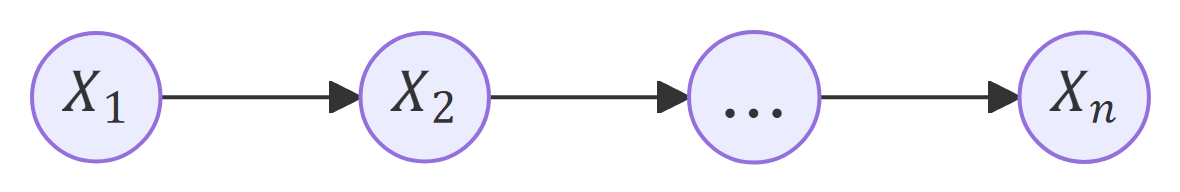
\includegraphics[width=3.08in,height=0.51in]{hmm_files/figure-latex/mermaid-figure-1.png}

Il \textbf{processo markoviano} è un caso specifico dei processi
stocastici, e in questo caso la proprietà principale è che lo stato
futuro dipende solamente dal suo presente e non dal passato. O, che
l'ossrevazione presente dipenda solo dal suo passato più recente.
L'ipotesi assuntiva è molto forte e permette di semplificare
drasticamente un modello di serie storiche. Infatti non servirà più
osservare l'intero passato per predire il futuro, ma basterà appena
avere le informazione sullo stato precedente. Ciò si basa su proprietà
base della probabilità, nel caso di un processo markoviano di primo
ordine, l'osservazione successiva dipenderà solamente dalla precedente:

\begin{definition}[Proprietà di
Markov]\protect\hypertarget{def-markov}{}\label{def-markov}

Sia \(\{X_t\}\) un processo stocastico. Allora \(\{X_t\}\) è markoviano
di ordine 1 se e solo se
\begin{equation}\phantomsection\label{eq-prop_markov}{
\Pr(X_t \mid X_{t-1},\dots,X_1)  =  \Pr(X_t \mid X_{t-1}) \qquad t \ge 2.
}\end{equation}

\end{definition}

Per la Definizione~\ref{def-markov}, tutte le future donazioni sono
indipendenti da quelle passate, ad eccezione di \(k\) osservazion più
recenti, dove \(k\) è il grado della catena markoviana:
\(x_{n+1} \perp x_{n-1} | x_n\).

Una catena di Markov omogenea (stazionaria nel tempo) è caratterizzata
da:

\begin{itemize}
\item
  la matrice di transizione \(\mathbf{A}\) con elementi
  \(a_{ij} = \Pr(X_t = j \mid X_{t-1} = i)\), per \(t \ge 2\);
\item
  il vettore di probabilità iniziali \(\boldsymbol{\pi}\) con
  \(\pi_i = \Pr(X_1 = i)\);
\item
  lo spazio degli stati finiti \(Z = \{1,\dots,K\}\).
\end{itemize}

\subsubsection{Proprietà strutturali}\label{proprietuxe0-strutturali}

Di seguito alcune proprietà importanti che verrano usate in seguito per
la descrizione e definizione degli Hidden Markov Model in generale e di
quello specificatamente utilizzato nel progetto.

\begin{definition}[Ergodicità (catene
omogenee)]\protect\hypertarget{def-ergodicity}{}\label{def-ergodicity}

Sia \(\{X_t\}_{t\ge 0}\) una catena di Markov a tempo discreto su spazio
degli stati finito \(Z\) con matrice di transizione \(\mathbf{A}\)
(costante nel tempo). Se la catena è irriducibile, aperiodica e
positivamente ricorrente, allora esiste ed è unica una distribuzione
stazionaria \(\boldsymbol{\pi}^*\) tale che
\(\boldsymbol{\pi}^* \mathbf{A} = \boldsymbol{\pi}^*\). Levin, Peres, e
Wilmer (2009).

\end{definition}

Il tempo di mixing misura quanto rapidamente la distribuzione della
catena ``dimentica'' le condizioni iniziali e si avvicina a
\(\boldsymbol{\pi}^*\).

\begin{definition}[Catena di Markov omogenea nel
tempo]\protect\hypertarget{def-homogeneous}{}\label{def-homogeneous}

Una catena di Markov discreta \(\{X_t\}_{t \ge 0}\) su spazio degli
stati finito \(Z\) si dice omogenea (o stazionaria nel tempo) se esiste
una matrice di transizione costante \(\mathbf{A}\) tale che, per ogni
\(t \ge 1\) e per ogni \(i,j \in Z\),
\begin{equation}\phantomsection\label{eq-matrice_costante}{
\Pr(X_t = j \mid X_{t-1} = i) = A_{ij},
}\end{equation}

ossia le probabilità di transizione non dipendono dal tempo.

\end{definition}

\begin{definition}[]\protect\hypertarget{def-stazionaria}{}\label{def-stazionaria}

Una distribuzione \(\boldsymbol{\pi}\) si dice \textbf{stazionaria} se
soddisfa \begin{equation}\phantomsection\label{eq-stazionaria}{
\boldsymbol{\pi}\,\mathbf{A} = \boldsymbol{\pi}, \qquad \boldsymbol{\pi}\,\mathbf{1} = 1,\ \ \boldsymbol{\pi}\!\ge\! \mathbf{0}.
}\end{equation}

\end{definition}

Una catena, invece, è detta non omogenea se la transizione al tempo
\(t\) è data da una matrice \(\mathbf{A}_t\) che può dipendere da \(t\)
o da covariate \(x_t\), cioè \(\mathbf{A}_t=\mathbf{A}(x_t)\). In
generale:

\begin{itemize}
\item
  non esiste una distribuzione stazionaria unica (indipendente dal
  tempo) che soddisfi
  \(\boldsymbol{\pi}\,\mathbf{A}_t=\boldsymbol{\pi}\) per tutti i \(t\);
\item
  si usa la nozione di ``ergodicità debole'': le distribuzioni indotte
  da condizioni iniziali diverse si avvicinano tra loro sotto opportune
  condizioni di contrazione.
\end{itemize}

\subsection{Hidden Markov Models (HMM)}\label{hidden-markov-models-hmm}

Come citato nel capitolo precedente, le catene markoviano sono molto
utili perché riescono a riassumere tutta la storia passata con appena
\(k\) passi precedenti, dove \(k\) è l'ordine della catena markoviana.
Quest'ipotesi permette di ridurre la fattorizzazione passando da
\begin{equation}\phantomsection\label{eq-markov_k}{
Pr(X_1, \dots, X_N) = Pr(X_1)Pr(X_2|X_1)Pr(X_3|X_2,X_1)\dots Pr(X_N+1|X_N,\dots, X_{N-k+1})\dots
}\end{equation}

In questo modo il modello è computazionalmente efficiente in quanto ha
bisogno di processare molta meno informazione.

Tuttavia, ciò non permette di modellare strutture più complesse, e in
questo caso bisogna raggirare la proprietà di Markov
(Definizione~\ref{def-markov}). Si introducono quindi delle variabili
latenti, ovvero delle variabili nascoste (\emph{hidden}), che non sono
osservate.

Vengono costituiti due stage/serie dipendenti tra loro: la prima serie è
costituita da una catena markoviana di \textbf{variabili latenti},
\(Z_t\) al tempo \(t\), che non possiamo osservare e che dipendono solo
dallo stato precedente, \(Z_{t-1}\) allo stato \(t-1\); la seconda
serie, invece, sono le \textbf{variabili osservate}, e la loro emissione
(distribuzione) dipende dallo stato latente.

Con parametri
\(\theta = (\boldsymbol{\pi}, \mathbf{A}, \boldsymbol{\phi})\) la
fattorizzazione congiunta è:
\begin{equation}\phantomsection\label{eq-hmm}{
\Pr(\mathbf{y}, \mathbf{z} \mid \theta)
= \Pr(z_1 \mid \boldsymbol{\pi}) \,\prod_{t=2}^{T} \Pr(z_t \mid z_{t-1}, \mathbf{A}) \,\prod_{t=1}^{T} \Pr(y_t \mid z_t, \boldsymbol{\phi}).
}\end{equation}

In aggiunta gli HMM permettono di modellare non solo una sequenza ma
anche molteplici. (Berry (2016))

\subsubsection{Estensioni degli HMM}\label{estensioni-degli-hmm}

Gli Hidden Markov Model possono essere estesi a problemi più
generalizzati. Si possono quindi rompere o adattare alcune parti della
sua struttura, come la matrice di transizione e le probabilità di
emissione. Facendo ciò si aumenta il grado di complessità del modello
perdendo leggermente la sua facile intuitività. Ma allo stesso tempo si
vanno a migliorare notevolmente le sue prestazioni e la sua adattabilità
al mondo reale. Di seguito vengono riportate alcune delle estensioni che
verranno poi implementato nel modello predittivo.

\paragraph{Emissioni flessibili}\label{sec-emissioni-flessibili}

Secondo Fan (2015), dato un HMM del primo ordine e che sia almeno
ergodico (Definizione~\ref{def-ergodicity}), allora si può definire una
famiglia esponenziale per la distribuzione condizionata alle
osservazioni, ovvero la distribuzione delle emissioni. Normalmente le
emissioni sono dei parametri della distribuzione di Poisson,
\(\lambda\), e della distribuzione Gaussiana, \(\mu\) o \(\sigma\). In
questo caso si andrebbe ad estendere il problema e si ipotizza una
famiglia esponenziale (vedi Sezione~\ref{sec-esponenziale}), che
racchiude sia la distribuzione Poisson che la Gaussiana. I parametri
della famiglia esponenziale, o della distribuzione scelta, non
dipenderebbero unicamente dallo stato latente, ma, dipenderebbero da dei
coefficienti \(\beta_k\) e da delle covariate \(W_{t}\). Le covariate
sono note, e possono cambiare nel tempo per l'individuo, permettendo al
modello una flessibilità temporale garantendo la stazionarietà. I
parametri da stimare diventano, quindi, i \(\beta_k\), e il loro valore
sarà condizionato allo stato latente. Di conseguenza, si produrrano
\(K\) GLM dove \(K\) è il numero di stati latenti.

\paragraph{Non omogeneità}\label{non-omogeneituxe0}

Per aumentare le performance del modello o per studiare a fondo le
dinamiche che possono influire nel cambio di stato, può essere
interessante aggiungere delle covariate nella matrice di transizione. Il
processo è simile a quello descritto nella sezione precedente (vedi
Sezione~\ref{sec-emissioni-flessibili}), tuttavia in questo caso non
garantiremmo più la proprietà di omogeneità (vedi
Definizione~\ref{def-homogeneous}).

\subsection{Inferenza bayesiana}\label{inferenza-bayesiana}

In un HMM l'approccio bayesiano fornisce un linguaggio naturale per
incorporare conoscenza a priori e per regolarizzare stime potenzialmente
instabili, soprattutto quando gli stati latenti sono pochi, i dati sono
rumorosi e le transizioni rare. L'idea è assegnare distribuzioni a
priori ai parametri chiave (probabilità iniziali sugli stati e matrice
di transizione) e poi combinarle con l'evidenza dei dati per ottenere le
posteriori. Tra le scelte più convenienti c'è la famiglia Dirichlet,
coniugata rispetto a vettori di probabilità: consente aggiornamenti
semplici e interpretazioni immediate in termini di ``pseudo-conteggi''.

Nel caso di stati finiti \(Z=\{1,\dots,K\}\), si pone una a priori
Dirichlet sul vettore delle probabilità iniziali e, riga per riga, sulle
transizioni: \[
\boldsymbol{\pi}\ \sim\ \mathrm{Dirichlet}(\boldsymbol{\alpha}_\pi),
\qquad
\mathbf{A}_{k,\cdot}\ \sim\ \mathrm{Dirichlet}(\boldsymbol{\alpha}_{A_k})\quad (k=1,\dots,K).
\]

Qui \(\boldsymbol{\alpha}_\pi\) e \(\boldsymbol{\alpha}_{A_k}\) sono
vettori di iperparametri positivi. La loro somma rappresenta la
``forza'' della prior: quanto più è grande, tanto più la prior
influenzerà la posteriore rispetto ai dati. Una prior simmetrica (tutte
le componenti uguali) è non informativa in senso debole; una prior
asimmetrica, invece, incorpora credenze specifiche, ad esempio maggiore
massa sullo stato ``inattivo'' per \(\boldsymbol{\pi}\) o maggiore
persistenza sulla diagonale per le righe di \(\mathbf{A}\).

Dati uno o più percorsi latenti \(z_{1:T}\) la coniugatezza della
Dirichlet corrisponde agli aggiornamenti per somma di conteggi. Se
indichiamo con \(c_i\) il numero di sequenze che iniziano nello stato
\(i\) e con \(n_{k j}\) il numero di transizioni osservate \(k\to j\),
allora \[
\boldsymbol{\pi}\mid z_{1} \ \sim\ \mathrm{Dirichlet}\big(\boldsymbol{\alpha}_\pi + \mathbf{c}\big),
\qquad
\mathbf{A}_{k,\cdot}\mid z_{1:T} \ \sim\ \mathrm{Dirichlet}\big(\boldsymbol{\alpha}_{A_k} + \mathbf{n}_{k,\cdot}\big),
\]

dove \(\mathbf{c}=(c_1,\dots,c_K)\) e
\(\mathbf{n}_{k,\cdot}=(n_{k1},\dots,n_{kK})\). Ne discendono formule
chiuse per media e predittiva: ad esempio la stima bayesiana (posterior
mean) del termine \(A_{k j}\) è \[
\mathbb{E}\!\left[A_{k j}\mid \text{dati}\right]
= \frac{\alpha_{A_k j} + n_{k j}}{\sum_{h=1}^K \big(\alpha_{A_k h} + n_{k h}\big)},
\]

e la probabilità di transizione ``one-step-ahead'' integra
automaticamente lo smoothing dei rari passaggi fuori diagonale. Questa
proprietà è particolarmente utile quando alcune transizioni sono poco o
per nulla osservate: la Dirichlet evita stime nulle e stabilizza
l'inferenza.

\begin{tcolorbox}[enhanced jigsaw, breakable, colframe=quarto-callout-note-color-frame, toprule=.15mm, title=\textcolor{quarto-callout-note-color}{\faInfo}\hspace{0.5em}{Intuizione sui parametri Dirichlet}, arc=.35mm, colback=white, bottomrule=.15mm, bottomtitle=1mm, colbacktitle=quarto-callout-note-color!10!white, toptitle=1mm, titlerule=0mm, opacityback=0, rightrule=.15mm, opacitybacktitle=0.6, leftrule=.75mm, left=2mm, coltitle=black]

Pensare a \(\boldsymbol{\alpha}\) come a pseudo-conteggi: una prior
simmetrica con \(\alpha=1\) per ciascuna voce equivale a ``una
osservazione virtuale'' per stato; aumentare la diagonale nelle righe di
\(\mathbf{A}\) equivale a credere che la catena tenda a permanere nello
stesso stato; usare \(\boldsymbol{\alpha}_\pi\) asimmetrica (ad esempio
più grande sulla componente dello stato 0) riflette l'aspettativa che
molte sequenze inizino ``a riposo''.

\end{tcolorbox}

Un tema tipico negli HMM è il ``label switching'': gli stati possono
scambiarsi etichette senza cambiare la verosimiglianza. Una prior
Dirichlet asimmetrica su \(\boldsymbol{\pi}\) e/o ``diagonale
rinforzata'' su \(\mathbf{A}\) spezza la simmetria, facilitando la
stabilità numerica e l'interpretazione dei profili latenti.

\begin{tcolorbox}[enhanced jigsaw, breakable, colframe=quarto-callout-tip-color-frame, toprule=.15mm, title=\textcolor{quarto-callout-tip-color}{\faLightbulb}\hspace{0.5em}{Scelte pratiche}, arc=.35mm, colback=white, bottomrule=.15mm, bottomtitle=1mm, colbacktitle=quarto-callout-tip-color!10!white, toptitle=1mm, titlerule=0mm, opacityback=0, rightrule=.15mm, opacitybacktitle=0.6, leftrule=.75mm, left=2mm, coltitle=black]

In problemi con forte persistenza conviene una prior sulle righe di
\(\mathbf{A}\) con massa più alta sulla diagonale; quando si sa che lo
stato iniziale è sbilanciato (molti ``inattivi''), una prior su
\(\boldsymbol{\pi}\) coerente con questa conoscenza accelera la
convergenza e riduce il label switching. Le concentrazioni totali
moderatamente piccole mantengono la prior ``debole'' lasciando ai dati
il grosso dell'inferenza.

\end{tcolorbox}

Dal punto di vista computazionale, l'uso di priors Dirichlet si integra
bene con schemi variazionali o EM, in quanto è coniugata alla
multinomiale. Le statistiche sufficienti sono i conteggi attesi di
occupazione e di transizione, ottenibili da forward--backward. (Murphy
(2012)) In variational Bayes o SVI, questi compaiono come termini attesi
nell'ELBO e consentono aggiornamenti stabili anche su dataset ampi,
mantenendo l'interpretabilità delle stime come ``conteggi osservati +
pseudo-conteggi''. (Bishop (2006))

\subsection{Teoria dell'algoritmo di Viterbi (caso
generale)}\label{sec-teoria_viterbi}

Nel caso classico di HMM con distribuzione iniziale
\(\boldsymbol{\pi}\), matrice di transizione \(\mathbf{A}\) ed emissioni
\(b_j(y_t)=\Pr(y_t\mid z_t{=}j)\), l'algoritmo di Viterbi cerca il
percorso a \emph{Maximum A Posteriori} (MAP), ovvero cerca lo stato
latente \(z_{0:T}^\star\) per la quale sia massima la sua probabilità
\begin{equation}\phantomsection\label{eq-MAP_z}{
z_{0:T}^\star=\arg\max_{z_{0:T}}\Pr(z_{0:T}\mid y_{0:T})
}\end{equation}

L'idea è trasformare questo problema globale in una sequenza di passi
locali grazie alla \textbf{programmazione dinamica}: invece di tenere
traccia di tutti i cammini possibili, si propaga nel tempo, per ciascuno
stato \(j\), il valore della ``miglior'' probabilità cumulativa che
termina in \(j\).

Per stabilità numerica si lavora in log-spazio. Si definisce quindi
\(\delta_t(j)\) come il massimo, tra tutti i cammini che arrivano a
\(t\) in \(j\), della log-probabilità congiunta fino a \(t\). Il passo
iniziale è: \begin{equation}\phantomsection\label{eq-viterbi_0}{
\delta_0(j)=\log \pi_j+\log b_j(y_0),
}\end{equation}

che combina la probabilità di partire nello stato \(j\) con la
verosimiglianza dell'osservazione iniziale. Il passo ricorsivo somma
l'evidenza al tempo \(t\) alla migliore prosecuzione dal tempo
precedente: \begin{equation}\phantomsection\label{eq-viterbi_t}{
\delta_t(j)=\log b_j(y_t)+\max_k\bigl\{\delta_{t-1}(k)+\log A_{k j}\bigr\}.
}\end{equation}

Per ricostruire il percorso, oltre ai valori \(\delta_t\) si memorizzano
i \emph{backpointer} \(\psi_t(j)\), cioè l'indice \(k\) che massimizza
l'espressione tra graffe. Al termine, si sceglie
\(z_T^\star=\arg\max_j \delta_T(j)\) e si risale a ritroso con
\(z_{t-1}^\star=\psi_t(z_t^\star)\) fino a \(t=1\). Dunque, Viterbi
calcola in avanti i punteggi ottimali e, alla fine, riassembla
all'indietro il cammino MAP.

Dal punto di vista computazionale, Viterbi è lineare nella lunghezza
della sequenza e quadratico nel numero di stati, con complessità
\(\mathcal{O}(T\,K^2)\) e memoria \(\mathcal{O}(T\,K)\) (per i
backpointer). In implementazione conviene usare sistematicamente la
forma log quando servono normalizzazioni, così da evitare
\emph{underflow} e garantire stabilità. Rabiner (1989)

I motivi per preferirlo sono pratici oltre che teorici: restituisce un
percorso ottimale globale rispetto alla \emph{loss} 0--1\footnote{La
  \emph{loss} 0-1 è una funzione di perdita che assegna una penalità
  pari a 1 se la predizione è errata, 0 se è corretta.} sulla sequenza
intera ed è efficiente anche su serie lunghe. Inoltre, è stabile
numericamente grazie al lavoro in log ed è soprattutto deterministico e
facilmente interpretabile, qualità preziose per analisi più approfondite
e successive personalizzazioni. Infine, si adatta senza sforzo a
contesti non omogenei o con covariate, come nel nostro HMM-GLM, perché
la dinamica ricorsiva resta invariata e cambia soltanto la parametricità
di \(\pi\), \(A\) ed emissioni.

\section{Il modello applicato alle
donazioni}\label{il-modello-applicato-alle-donazioni}

\subsection{Pyro}\label{sec-pyro}

Dopo la parte teorica, in questo capitolo parleremo della applicazione
della teoria ai dati sulle donazioni di sangue. Se nel precedentemente
capitolo era stato utilizzato quasi totalmente il linguaggio di
programmazione statistica R con i pacchetti \texttt{tidyverse} e
\texttt{tidymodels}, in questo capitolo i modelli verranno sviluppati
attraverso il linguaggio di programmazione Python e il pacchetto
\texttt{Pyro}.

Pyro è un linguaggio universale di programmazione probabilistica scritto
in Python e costruito con \texttt{PyTorch} nel \emph{backend}. Ma a cosa
serve? Secondo Bingham et al. (2018), Pyro permette di scrivere in modo
facile e flessibile modelli probablistici, tra cui modelli di \emph{deep
learning} e bayesiani. I punti di forza di Pyro sono i seguenti:

\begin{itemize}
\item
  universale, in quanto può rappresentare qualsiasi distribuzione di
  probabilità computabile;
\item
  scalabile, ideale per lavorare su grandi \emph{data set};
\item
  minimale, è costituito da un piccolo ma potente \emph{core}, e
\item
  flexible, è facilmente automatizzabile, ma al contempo controllabile,
  quando necessario.
\end{itemize}

Ovviamente non è l'unico strumento utilizzabile per costruire i modelli
mostrati successivamente. Una valida alternativa è \texttt{stan},
implementata in R attraverso i pacchetti come \texttt{rstan}.

\subsection{Dati e covariate}\label{sec-covariate}

I dati sono stati inizialmente elaborati in R, succesivamente esportati
in formato tabellare (CSV), ed infine importati in Python. L'obiettivo
era quello di ottenere dei dati in formato tabulare dove ogni riga
rappresentasse il donatore e con una colonna per ogni anno
d'osservazione, contenente il numero di donazioni effettuate in quello
specifico anno. Infine, altre colonne con le informazioni sul donatore,
come l'anno di nascita, il genere e l'età. Successivamente, i dati sono
stati modificati ulteriormente addattandoli all'ambiente di sviluppo in
Python.

Abbiamo ottenuto così un un pannelo longitudinale con \(N = 9236\)
donatori, le loro donazioni negli anni 2009-2023 (\(T = 15\)) e le
covariate con le informazioni demografiche sul donatore. Per la
modellizzazione dei dati si è diviso il dataset iniziale in 4 dataset
più piccoli:

\begin{enumerate}
\def\labelenumi{\arabic{enumi}.}
\item
  il primo contenente le colonne costituite dai conteggi annuali per
  donatore;
\item
  il secondo contenente le covariate necessarie per la determinazione
  delle probabilità iniziali;
\item
  il terzo costituito dalle covariate per la matrice di transizione,
\item
  e l'ultimo contenente le covariate per i modelli GLM.
\end{enumerate}

\subsubsection{Dataset sulle osservazioni delle
donazioni}\label{dataset-sulle-osservazioni-delle-donazioni}

Il primo dataset sarà costituito da sole \(y_t \in \{0,1,2,3,4\}\), dove
\(t\) è il tempo. Il limite superiore del dominio dei dati è dovuto a
una regola clinica: ovvero un donatore può al più donare 4 volte
all'anno per sangue intero. Questo ha portato all'utilizzo di
distribuzioni probabilistiche improrie, ovvero che non erano contemplate
per la natura dei dati, ma che a causa della loro forma, si adattavano
molto bene al caso nostro.

La distribuzione di probabilità più appropriata sarebbe stata infatti
una distribuzione binomiale, o una categorica. Tuttavia la distribuzione
di Poisson era quella che meglio si adattava i dati, anche se è stata
troncata sulla coda destra a causa della regola clinica.

\subsubsection{Dataset con le covariate per le probabilità
iniziali}\label{dataset-con-le-covariate-per-le-probabilituxe0-iniziali}

Il secondo dataset sarà usato per calcolare
\(\pi = Pr(Z_{n,1} \mid X_{n,1}^{\pi})\), ovvero la probabilità
dell'individuo \(n\) di iniziare nello stato \(k\), date le covariate
\(X_{n,1}^{\pi}\), dove \(X_{n,1}^{\pi}\) è una matrice di dimensione
\(N, P_\pi\) con \(p_\pi\) il numero di covariate utilizzate.

Le probabilità iniziali vengono calcolate solo per il primo stato.
Devono, perciò, sfruttare delle informazioni disponibili al tempo \(1\).
Le sue covariate saranno di conseguenza statiche.

La sua importanza è relativa, infatti grazie alla matrice di
transizione, le unità si sposteranno tra gli stati e assumeranno lo
stato che più gli si adatta allo specifico tempo \(t\).

\subsubsection{Dataset con le covariate per la matrice di
transizione}\label{dataset-con-le-covariate-per-la-matrice-di-transizione}

Il modello che verrà sviluppato in questo capitolo è diverso da un
classico \emph{hidden markov model} e non possiederà tutte le sue
proprietà. In specifico non gode della proprietà di omogeneità, ovvero
non è un modello stazionario (vedi Definizione~\ref{def-homogeneous}).
Non ci aspettiamo che un donatore appartenga sempre allo stato, ovvero
che sia propenso sempre allo stesso modo di donare. Riteniamo che esso
dipenda da fattori esterni che influenzino il suo comportamento. Questi
fattori non sono fissi e cambiano nel tempo. Sarà dunque necessario
includere delle covariate dinamiche, che cambiano nel tempo, come l'età
del donatore. Otterremo dunque una matrice di 3 dimensioni \(N, P_A, T\)
dove \(N\) è il numero di donatori, \(P_A\) il numero di variabili usate
e \(T\) gli anni usati dal modello.

Le covariate utilizzate saranno l'età e gli anni del covid. Analizzando
l'età, si osserva come il suo andamento non sia lineare. Al crescere
dell'età non si può assertare né che il numero di donazioni sia in
aumento, né che il numero di donazioni sia in diminuzione. Infatti agli
estremi, ovvero nelle fasce d'età più giovani e più anziane si
osserveranno un numero di donazioni minore mentre nella fascia centrale,
un numero di donazioni maggiore. Sia \(\mathbf{X}\) e \(\mathbf{Y}\) due
vettori (o matrici) e sia \(\mathbf{A}\) una matrice di trasformazione
tale che \[
\mathbf{Y} = \mathbf{A}\,\mathbf{X} + \boldsymbol{\varepsilon}.
\]

Il nostro obiettivo è trovare \[
\arg\min_{\mathbf{A}\in\mathbb{R}^{q\times p}}   \|\mathbf{Y}-\mathbf{A}\mathbf{X}\|^2.
\]

Le opzioni possibili per gestire il suddetto problema sono molteplici,
dalle più semplici alle più complesse.\\
Tra le principali strategie si possono citare:

\begin{itemize}
\item
  \textbf{aggiunta di potenze della variabile}: ad esempio includendo
  termini quadratici o cubici dell'età
  (\(\text{età}^2, \text{età}^3, \dots\)) per catturare eventuali
  relazioni non lineari;
\item
  \textbf{categorizzazione della variabile}: suddividere l'età in fasce
  (es. 18--24, 25--34, 35--44, \ldots) e introdurre variabili dummy per
  ciascuna categoria, consentendo al modello di apprendere effetti
  differenti per ciascun gruppo;
\item
  \textbf{funzioni spline}: utilizzare spline lineari o cubic spline per
  rappresentare in modo flessibile l'andamento non lineare dell'età,
  mantenendo al contempo una continuità nei punti di raccordo;
\item
  \textbf{altri approcci di regolarizzazione o riduzione di
  dimensionalità}: ad esempio penalizzazioni (ridge, lasso) per evitare
  overfitting in presenza di molte trasformazioni, oppure tecniche di
  smooth fitting per controllare la complessità del modello.
\end{itemize}

Queste trasformazioni permettono di modellare meglio l'effetto dell'età,
evitando di imporre una relazione lineare troppo restrittiva e
garantendo al tempo stesso una maggiore flessibilità nella costruzione
della matrice di transizione.

Tra le diverse strategie illustrate, in questo lavoro si è deciso di
adottare la \textbf{categorizzazione della variabile età}.\\
Questa scelta consente di distinguere in modo chiaro le diverse fasce
d'età dei donatori, mantenendo al tempo stesso un modello
interpretabile. In particolare, le categorie permettono di osservare
come il comportamento donazionale vari nei diversi gruppi, evidenziando
ad esempio differenze tra i donatori più giovani, quelli in età
intermedia e i più anziani.\\
In questo modo si ottiene un compromesso tra semplicità e capacità di
rappresentare l'andamento non lineare della variabile, evitando di
introdurre complessità eccessiva tramite spline o polinomi di grado
elevato.

Durante la pandemia da coronavirus SARS-CoV-2 la propensione a donare e
le sue motivazioni sono cambiate molto. Riteniamo quindi di dovere
aggiungere quest'informazione al modello e manipolare la serie storica
in questo momento storico in modo a se stante. Infatti grazie
all'introduzione di questa covariate si possono osservare in quegli
anni, un profondo cambiamento del trend.

\subsubsection{Dataset con le covariate per i GLM}\label{sec-emissioni}

Attraverso le probabilità iniziali e la matrice di transizione possiamo
risalire allo stato latente dell'individuo lungo la sua serie storica.
Con l'obbietivo di predire il valore atteso della prossima donazione, lo
stato latente più importante che ci interesserà conoscere, sarà l'ultimo
stato latente, ovvero lo stato che ci dirà quale dei \(K\) diversi
modelli utilizzare. Il HMM-GLM ha esattamente questo di differenza
confronto un normale HMM, l'HMM-GLM non restituisce un \emph{rate}, o il
parametro di una qualsiasi distribuzione; ma restituisce l'indicazione a
quale modello usare. Infatti, ipotizziamo che il modello generatore dei
dati sia significativamente diverso tra i 3 diversi \emph{pattern} di
dontari. E non è una differenza fissa/statica, ma una differenza molto
più complessa, che è influenzata anche da altri fattori. Per questo, si
ritene opportuno usare 3 modelli diversi per modellare e predire le
future donazioni di sangue.

Le covariate scelte in questo caso sono un incrocio tra covariate
statiche e dinamiche. Le variabili scelte sono il genere, le fasce d'età
e il periodo covid.

\subsection{Componenti del Modello}\label{componenti-del-modello}

Il modello, come citato in Sezione~\ref{sec-pyro}, è definito tramite
Pyro. Si ritiene che sia importante esplicitare il codice, tanto quanto
la stesura di una formula matematica. Mediante la lettura del codice si
comprende a pieno le potenzialità di Pyro e la struttura del modello.

Il numero di stati latenti, \texttt{K}, è stato fissato a 3. Quindi,
\(z_{n,t} \in \{0,1,2\}\), e non sono osservate. La loro interpretazione
reale sarà il profilo di donatore, ovvero se sarà un donatore frequente,
occasionale o sporadico.

Le osservazioni, \(y_{n,t} \in \mathbb{N}\), sono conservate nella
variabile \texttt{obs}, che è una matrice di dimensione \texttt{N},
\texttt{T} e assume valori in \([0,4]\). Come spiegato nel capitolo
precedente (vedi Sezione~\ref{sec-covariate}), sono presenti altre tre
matrici composte da:

\begin{itemize}
\item
  covariate sulle probabilità inziali,
  \(W_\pi \in \mathbb{R}^{K\times 2}\);
\item
  covariate sulla matrice di transizione,
  \(W_A \in \mathbb{R}^{K\times K \times 8}\); e
\item
  covariate sulle emissioni,
  \(\beta_{em} \in \mathbb{R}^{K \times (1+9)}\), che in questo caso
  saranno le covariate dei \(K\) diversi modelli.
\end{itemize}

\subsubsection{Approccio Bayesiano}\label{sec-bayesiano}

Abbiamo adottato un approccio bayesiano per le componenti che governano
le probabilità iniziali e le transizioni dell'HMM, usando prior di tipo
Dirichlet sulle intercette e lasciando stimare per MAP (via
\texttt{pyro.param}) le pendenze che modulano l'effetto delle covariate.
In particolare:

\begin{itemize}
\item
  distribuzione iniziale:
  \(\pi_{\text{base}} \sim \text{Dirichlet}(\boldsymbol{\alpha}_\pi)\)
  con \(\boldsymbol{\alpha}_\pi\) asimmetrica per spezzare la simmetria
  delle etichette e incorporare la conoscenza a priori sull'elevata
  prevalenza dello ``stato inattivo'' (non-donatore), dovuto al fatto
  che al tempo \(t=0\), ancora molti dei donatori non avevano iniziato a
  donare;
\item
  matrice di transizione: per ciascuna riga \(k\),
  \(A_{\text{base}}[k,\cdot] \sim \text{Dirichlet}(\boldsymbol{\alpha}_{A_k})\).
  Abbiamo valutato sia una a priori non informativa (simmetrica) sia una
  a priori ``diagonale'' (con massa concentrata sulla permanenza
  \(k \to k\)).
\end{itemize}

Motivazioni per l'approccio bayesiano:

\begin{itemize}
\item
  identificabilità pratica: una prior asimmetrica su \(\pi\) mitiga il
  \emph{label switching} e rende più stabile il confronto tra fit
  riavviati con semi diversi;
\item
  inferenza scalabile: l'uso della variazionale stocastica con
  enumerazione esatta delle variabili discrete
  (\texttt{TraceEnum\_ELBO}) riduce la varianza del gradiente e consente
  di trattare in modo efficiente le catene latenti \(z_{n,t}\) (Hoffman
  et al. (2013));
\item
  coerenza interpretativa: la combinazione ``prior diagonale'' su \(A\)
  e Poisson/Gamma sulle emissioni porta a tre profili comportamentali
  stabili (non-, leggero, frequente donatore), con transizioni credibili
  e facilmente comunicabili.
\end{itemize}

\subsubsection{Definizione del modello}\label{sec-def_modello}

Il modello è caratterizzato da due cicli annidati tra loro, uno sul
numero di osservazioni e l'altro sulla serie temporale. Questi cicli
sono caratterizzati da un passo base e un passo iterativo. Potremmo
definire l'algoritmo così come segue:

\emph{Passo base} \(n\):

\begin{enumerate}
\def\labelenumi{\arabic{enumi}.}
\item
  campionamento delle a priori e conversione in base logaritmica per le
  variabili \(\pi_{\text{base},k}\) e \(A_{\text{base},kj}\)
\item
  calcolo dei coeffienti tramite la matrice delle covariate per i
  parametri \(W_{\pi,k}\), \(W_{A,kj}\) e \(\beta_{em,}\).
\end{enumerate}

\emph{Passo iterativo} \(n\):

\emph{Passo base} \(t\):

\begin{enumerate}
\def\labelenumi{\arabic{enumi}.}
\setcounter{enumi}{2}
\item
  Calcolo delle probabilità inziale dell'individuo di iniziare la sua
  traiettoria nello stato \(k\), tramite la formula
  \begin{equation}\phantomsection\label{eq-prob_iniziali}{
  \Pr(z_{n,0}=k \mid x^\pi_n) =
  \text{softmax}_k \big( \log \pi_{\text{base},k} + W_{\pi,k} \cdot x^\pi_n \big)
  }\end{equation}

  e campionamento dello stato da tali probabilità.
\item
  Calcolo del parametro \(\log (\mu_{n,t}^{\text{em}})\) corrispondente
  al logaritmo del valore atteso di donare al tempo \(t=0\).
  Campionamente di \(y_0\) dalla distribuzione di Poisson con il
  parametro appena calcolato.
\end{enumerate}

\emph{Passo iterativo} \(t\):

\begin{enumerate}
\def\labelenumi{\arabic{enumi}.}
\setcounter{enumi}{4}
\item
  Calcolo delle probabilità di transizione al tempo \(t\) sfruttando la
  matrice di transizione calcolata nel passo base di \(n\) e pesata per
  le informazioni che si hanno a disposizione per l'unità \(n\) al tempo
  \(t\). Attraverso questa formula
  \begin{equation}\phantomsection\label{eq-trans_matrix}{
   \Pr(z_{n,t}=j \mid z_{n,t-1}=k, \ x^A_{n,t}) =
   \text{softmax}_j \big( \log A_{\text{base},kj} + W_{A,kj} \cdot x^A_{n,t} \big)
   }\end{equation}

  si campiona la probabilià che l'unità \(n\) occupi lo stato \(j\) al
  passo \(t\) sapendo che al passo \(t-1\) occupava lo stato \(k\).
\item
  Dato lo stato \(j\), calcolato al punto precedente, campionamento del
  numero di donazioni al tempo \(t\):
  \begin{equation}\phantomsection\label{eq-emissioni}{
   y_{n,t} \mid z_{n,t}=k \sim \text{Poisson}\Big(
     \exp\Big( X^{em}_{n,t} \mathbf{\beta_{em,k}}
     \Big)
   \Big)
   }\end{equation}
\end{enumerate}

\begin{codelisting}

\caption{\label{lst-model}Definizione del modello in Pyro}

\centering{

\begin{Shaded}
\begin{Highlighting}[]
\NormalTok{K      }\OperatorTok{=} \DecValTok{3}                      \CommentTok{\# Number of latent states}
\NormalTok{C\_pi   }\OperatorTok{=}\NormalTok{ cov\_init.shape[}\DecValTok{1}\NormalTok{]      }\CommentTok{\# Initial{-}state covariates}
\NormalTok{C\_A    }\OperatorTok{=}\NormalTok{ cov\_tran.shape[}\DecValTok{2}\NormalTok{]      }\CommentTok{\# Transition covariates}
\NormalTok{C\_em   }\OperatorTok{=}\NormalTok{ cov\_emission.shape[}\DecValTok{2}\NormalTok{]  }\CommentTok{\# Emission covariates}

\CommentTok{\# Dirichlet prior}
\NormalTok{alpha\_pi }\OperatorTok{=}\NormalTok{ torch.tensor([}\FloatTok{5.}\NormalTok{, }\FloatTok{2.}\NormalTok{, }\FloatTok{1.}\NormalTok{])}
\NormalTok{alpha\_A  }\OperatorTok{=}\NormalTok{ torch.ones((K, K))}

\AttributeTok{@config\_enumerate}
\KeywordTok{def}\NormalTok{ model(obs, x\_pi, x\_A, x\_em):}
\NormalTok{    N, T }\OperatorTok{=}\NormalTok{ obs.shape}

    \CommentTok{\# 1) Priors/parameters for initial and transition distribution}
\NormalTok{    pi\_base }\OperatorTok{=}\NormalTok{ pyro.sample(}\StringTok{"pi\_base"}\NormalTok{, dist.Dirichlet(alpha\_pi))}
\NormalTok{    A\_base }\OperatorTok{=}\NormalTok{ pyro.sample(}\StringTok{"A\_base"}\NormalTok{, dist.Dirichlet(alpha\_A).to\_event(}\DecValTok{1}\NormalTok{))}
\NormalTok{    log\_pi\_base }\OperatorTok{=}\NormalTok{ pi\_base.log()}
\NormalTok{    log\_A\_base  }\OperatorTok{=}\NormalTok{ A\_base.log()}

    \CommentTok{\# 2) Slope coefficients for initial and transition covariates }
    \CommentTok{\# and State{-}specific GLM emission coefficients (learned)}
\NormalTok{    W\_pi }\OperatorTok{=}\NormalTok{ pyro.param(}\StringTok{"W\_pi"}\NormalTok{, torch.zeros(K, C\_pi))}
\NormalTok{    W\_A  }\OperatorTok{=}\NormalTok{ pyro.param(}\StringTok{"W\_A"}\NormalTok{, torch.zeros(K, K, C\_A))}
\NormalTok{    beta\_em }\OperatorTok{=}\NormalTok{ pyro.param(}\StringTok{"beta\_em"}\NormalTok{, torch.zeros(K, C\_em)) }

    \ControlFlowTok{with}\NormalTok{ pyro.plate(}\StringTok{"seqs"}\NormalTok{, N):}
        \CommentTok{\# Initial hidden state probabilities: depend on x\_pi via W\_pi}
\NormalTok{        logits0 }\OperatorTok{=}\NormalTok{ log\_pi\_base }\OperatorTok{+}\NormalTok{ (x\_pi }\OperatorTok{@}\NormalTok{ W\_pi.T)}
\NormalTok{        z\_prev }\OperatorTok{=}\NormalTok{ pyro.sample(}\StringTok{"z\_0"}\NormalTok{,}
\NormalTok{                             dist.Categorical(logits}\OperatorTok{=}\NormalTok{logits0),}
\NormalTok{                             infer}\OperatorTok{=}\NormalTok{\{}\StringTok{"enumerate"}\NormalTok{: }\StringTok{"parallel"}\NormalTok{\})}

        \CommentTok{\# Emission at t=0: state{-}specific GLM on covariates x\_em}
\NormalTok{        log\_mu0 }\OperatorTok{=}\NormalTok{ (x\_em[:, }\DecValTok{0}\NormalTok{, :] }\OperatorTok{*}\NormalTok{ beta\_em[z\_prev, :]).}\BuiltInTok{sum}\NormalTok{(}\OperatorTok{{-}}\DecValTok{1}\NormalTok{)}
\NormalTok{        pyro.sample(}\StringTok{"y\_0"}\NormalTok{, dist.Poisson(log\_mu0.exp()), obs}\OperatorTok{=}\NormalTok{obs[:, }\DecValTok{0}\NormalTok{])}

        \CommentTok{\# For t = 1 ... T{-}1, update state and emit}
        \ControlFlowTok{for}\NormalTok{ t }\KeywordTok{in} \BuiltInTok{range}\NormalTok{(}\DecValTok{1}\NormalTok{, T):}
\NormalTok{            x\_t }\OperatorTok{=}\NormalTok{ x\_A[:, t, :]}
\NormalTok{            logitsT }\OperatorTok{=}\NormalTok{ log\_A\_base[z\_prev] }\OperatorTok{+}\NormalTok{ (W\_A[z\_prev] }\OperatorTok{*}\NormalTok{ x\_t[:,}\VariableTok{None}\NormalTok{,:]).}\BuiltInTok{sum}\NormalTok{(}\OperatorTok{{-}}\DecValTok{1}\NormalTok{)}
\NormalTok{            z\_t }\OperatorTok{=}\NormalTok{ pyro.sample(}\SpecialStringTok{f"z\_}\SpecialCharTok{\{}\NormalTok{t}\SpecialCharTok{\}}\SpecialStringTok{"}\NormalTok{,}
\NormalTok{                             dist.Categorical(logits}\OperatorTok{=}\NormalTok{logitsT),}
\NormalTok{                             infer}\OperatorTok{=}\NormalTok{\{}\StringTok{"enumerate"}\NormalTok{: }\StringTok{"parallel"}\NormalTok{\})}

            \CommentTok{\# Emission: state{-}specific GLM at time t}
\NormalTok{            log\_mu\_t }\OperatorTok{=}\NormalTok{ (x\_em[:, t, :] }\OperatorTok{*}\NormalTok{ beta\_em[z\_t, :]).}\BuiltInTok{sum}\NormalTok{(}\OperatorTok{{-}}\DecValTok{1}\NormalTok{)}
\NormalTok{            pyro.sample(}\SpecialStringTok{f"y\_}\SpecialCharTok{\{}\NormalTok{t}\SpecialCharTok{\}}\SpecialStringTok{"}\NormalTok{,}
\NormalTok{                        dist.Poisson(log\_mu\_t.exp()),}
\NormalTok{                        obs}\OperatorTok{=}\NormalTok{obs[:, t])}
\NormalTok{            z\_prev }\OperatorTok{=}\NormalTok{ z\_t}
\end{Highlighting}
\end{Shaded}

}

\end{codelisting}%

\subsubsection{Definizione del guide}\label{sec-guide}

Il guide specifica la famiglia variazionale \(q(\cdot)\) utilizzata da
SVI (\emph{stochastic variational inferance}) per approssimare la
posteriore. Qui scegliamo una approssimazione ``a massa puntuale''
(Delta) per i soli nodi continui latenti del modello, cioè le intercette
della distribuzione iniziale e della matrice di transizione:
\(q(\pi_{\text{base}})=\delta(\pi_{\text{base}}-\hat\pi)\) e
\(q(A_{\text{base}})=\delta(A_{\text{base}}-\hat A)\).

Le variabili discrete \(z_{n,t}\) non compaiono nel guide perché vengono
enumerate esattamente nel modello (\texttt{@config\_enumerate}), e i
coefficienti \(W_\pi\), \(W_A\), \(\beta_{\text{em}}\) sono stimati come
parametri deterministici (\texttt{pyro.param}). In termini teorici, si
massimizza l'ELBO scegliendo una famiglia variazionale degenere (MAP)
per \(\pi_{\text{base}}\) e \(A_{\text{base}}\), in modo da semplificare
l'ottimizzazione e stabilizzare l'identificazione. Anche se, in questo
modo, non si quantifica l'incertezza.

I vincoli simplex (\texttt{dist.constraints.simplex}) garantiscono che
\(\hat\pi\) e ciascuna riga di \(\hat A\) siano probabilità valide (non
negative e a somma unitaria). L'inizializzazione deve già rispettare il
vincolo: normalizziamo \(\boldsymbol{\alpha}_\pi\) per ottenere un punto
di partenza ammissibile per \(\pi_q\), mentre per \(A_q\) usiamo una
matrice ``diagonale rinforzata'' rinormalizzata per riga, che favorisce
la persistenza.

\begin{codelisting}

\caption{\label{lst-guide}Definizione del Guide in Pyro}

\centering{

\begin{Shaded}
\begin{Highlighting}[]
\KeywordTok{def}\NormalTok{ guide(obs, x\_pi, x\_A, x\_em):}
\NormalTok{    pi\_q }\OperatorTok{=}\NormalTok{ pyro.param(}
        \StringTok{"pi\_base\_map"}\NormalTok{,}
\NormalTok{        alpha\_pi,}
\NormalTok{        constraint}\OperatorTok{=}\NormalTok{dist.constraints.simplex}
\NormalTok{    )}

    \CommentTok{\# Each row: simplex for state{-}to{-}state transitions}
\NormalTok{    A\_init }\OperatorTok{=}\NormalTok{ torch.eye(K) }\OperatorTok{*}\NormalTok{ (K }\OperatorTok{{-}} \FloatTok{1.}\NormalTok{) }\OperatorTok{+} \FloatTok{1.}
\NormalTok{    A\_init }\OperatorTok{=}\NormalTok{ A\_init }\OperatorTok{/}\NormalTok{ A\_init.}\BuiltInTok{sum}\NormalTok{(}\OperatorTok{{-}}\DecValTok{1}\NormalTok{, keepdim}\OperatorTok{=}\VariableTok{True}\NormalTok{)}
\NormalTok{    A\_q }\OperatorTok{=}\NormalTok{ pyro.param(}
        \StringTok{"A\_base\_map"}\NormalTok{,}
\NormalTok{        A\_init,}
\NormalTok{        constraint}\OperatorTok{=}\NormalTok{dist.constraints.simplex}
\NormalTok{    )}

\NormalTok{    pyro.sample(}\StringTok{"pi\_base"}\NormalTok{, dist.Delta(pi\_q).to\_event(}\DecValTok{1}\NormalTok{))}
\NormalTok{    pyro.sample(}\StringTok{"A\_base"}\NormalTok{,  dist.Delta(A\_q).to\_event(}\DecValTok{2}\NormalTok{))}
\end{Highlighting}
\end{Shaded}

}

\end{codelisting}%

\subsubsection{Allenamento del modello}\label{sec-allenamento}

L'addestramento dell'HMM-GLM è stato condotto con un approccio bayesiano
variazionale. Il modello principale è stato allenato su tutti i dati, in
modo da avere un modello in produzione il più performante possibile. In
area di sviluppo, invece, il dataset è stato suddiviso in train/test con
split 90/10, stratificando per genere e fascia d'età al tempo iniziale e
fissando il seed a 42, per garantire la riproducibilità. Ottenendo così
due dataset, il dataset con i dati d'allenamento, \emph{train}
\(N=8308\), e il dataset con i dati di test, \emph{test} \(N=928\).

Le covariate, come visto anche nella Sezione~\ref{sec-def_modello}, sono
state progettate in tre blocchi coerenti con le tre componenti del
modello: iniziali \(x^\pi\in\mathbb{R}^{3}\) (intercetta,
\texttt{birth\_year\_norm} in z-score, \texttt{gender\_code} F=1/M=0),
transizioni \(x^A_t\in\mathbb{R}^{8}\) (intercetta; fasce d'età one-hot
con baseline 18--24 \texttt{age\_class}; indicatore \texttt{covid\_year}
per 2020--2022), ed emissioni \(x^{\text{em}}_t\in\mathbb{R}^{9}\)
(intercetta; \texttt{gender}; stesse dummies d'età;
\texttt{covid\_year}).

\begin{tcolorbox}[enhanced jigsaw, breakable, colframe=quarto-callout-note-color-frame, toprule=.15mm, title=\textcolor{quarto-callout-note-color}{\faInfo}\hspace{0.5em}{Scelta del numero di parametri}, arc=.35mm, colback=white, bottomrule=.15mm, bottomtitle=1mm, colbacktitle=quarto-callout-note-color!10!white, toptitle=1mm, titlerule=0mm, opacityback=0, rightrule=.15mm, opacitybacktitle=0.6, leftrule=.75mm, left=2mm, coltitle=black]

Il numero di stati latenti è stato fissato a \(K=3\) per ragioni di
interpretabilità e stabilità numerica. Inoltre, la scelta è stata
giustificata anche dal \emph{Bayesian Information Criterion}, BIC Wit,
Heuvel, e Romeyn (2012). Il BIC è un criterio per la selezione del
modello statistico da usare basato sulla funzione di verosimiglianza ma
che viene penalizzato all'aumentare del numero di parametri e dalla
scarsezza del numero di osservazioni ed è definito come segue:
\begin{equation}\phantomsection\label{eq-bic}{
\text{BIC} = k\ln(n) - 2\ln(\widehat L)
}\end{equation}

dove \(\widehat L\) è la funzione di verosimiglianza, \(n\) il numero di
osservazioni e \(k\) il numero di parametri. Il motivo per la quale si
usa il logaritmico sul numero di ossarvazioni, \(\ln(n)\), è dovuto alla
\emph{maledizione delle dimensionalità} (Bellman (1957)): all'aumentare
del numero di parametri è necessario un numero esponenzialmente
crescente di osservazioni per mantenere invariato il livello di
incertezza nelle stime.

Osservando il grafico Figura~\ref{fig-bic}, si nota, come il criterio
BIC raggiunga il suo massimo con il numero di stati pari a 3. Nel
grafico, non viene utilizzata la formula precedentemente descritta, ma
una sua variante in modo da comparare facilmente l'assenza dell'utlizzo
di un parametro di penalizzazione nella \emph{likelihood} e la sua
aggiunta. La formula usata è la seguente:

\begin{equation}\phantomsection\label{eq-bic_like}{
\text{BIC-like} = \ln(\widehat L) - \frac{1}{2} k \ln(n)
}\end{equation}

\begin{figure}[H]

\centering{

\pandocbounded{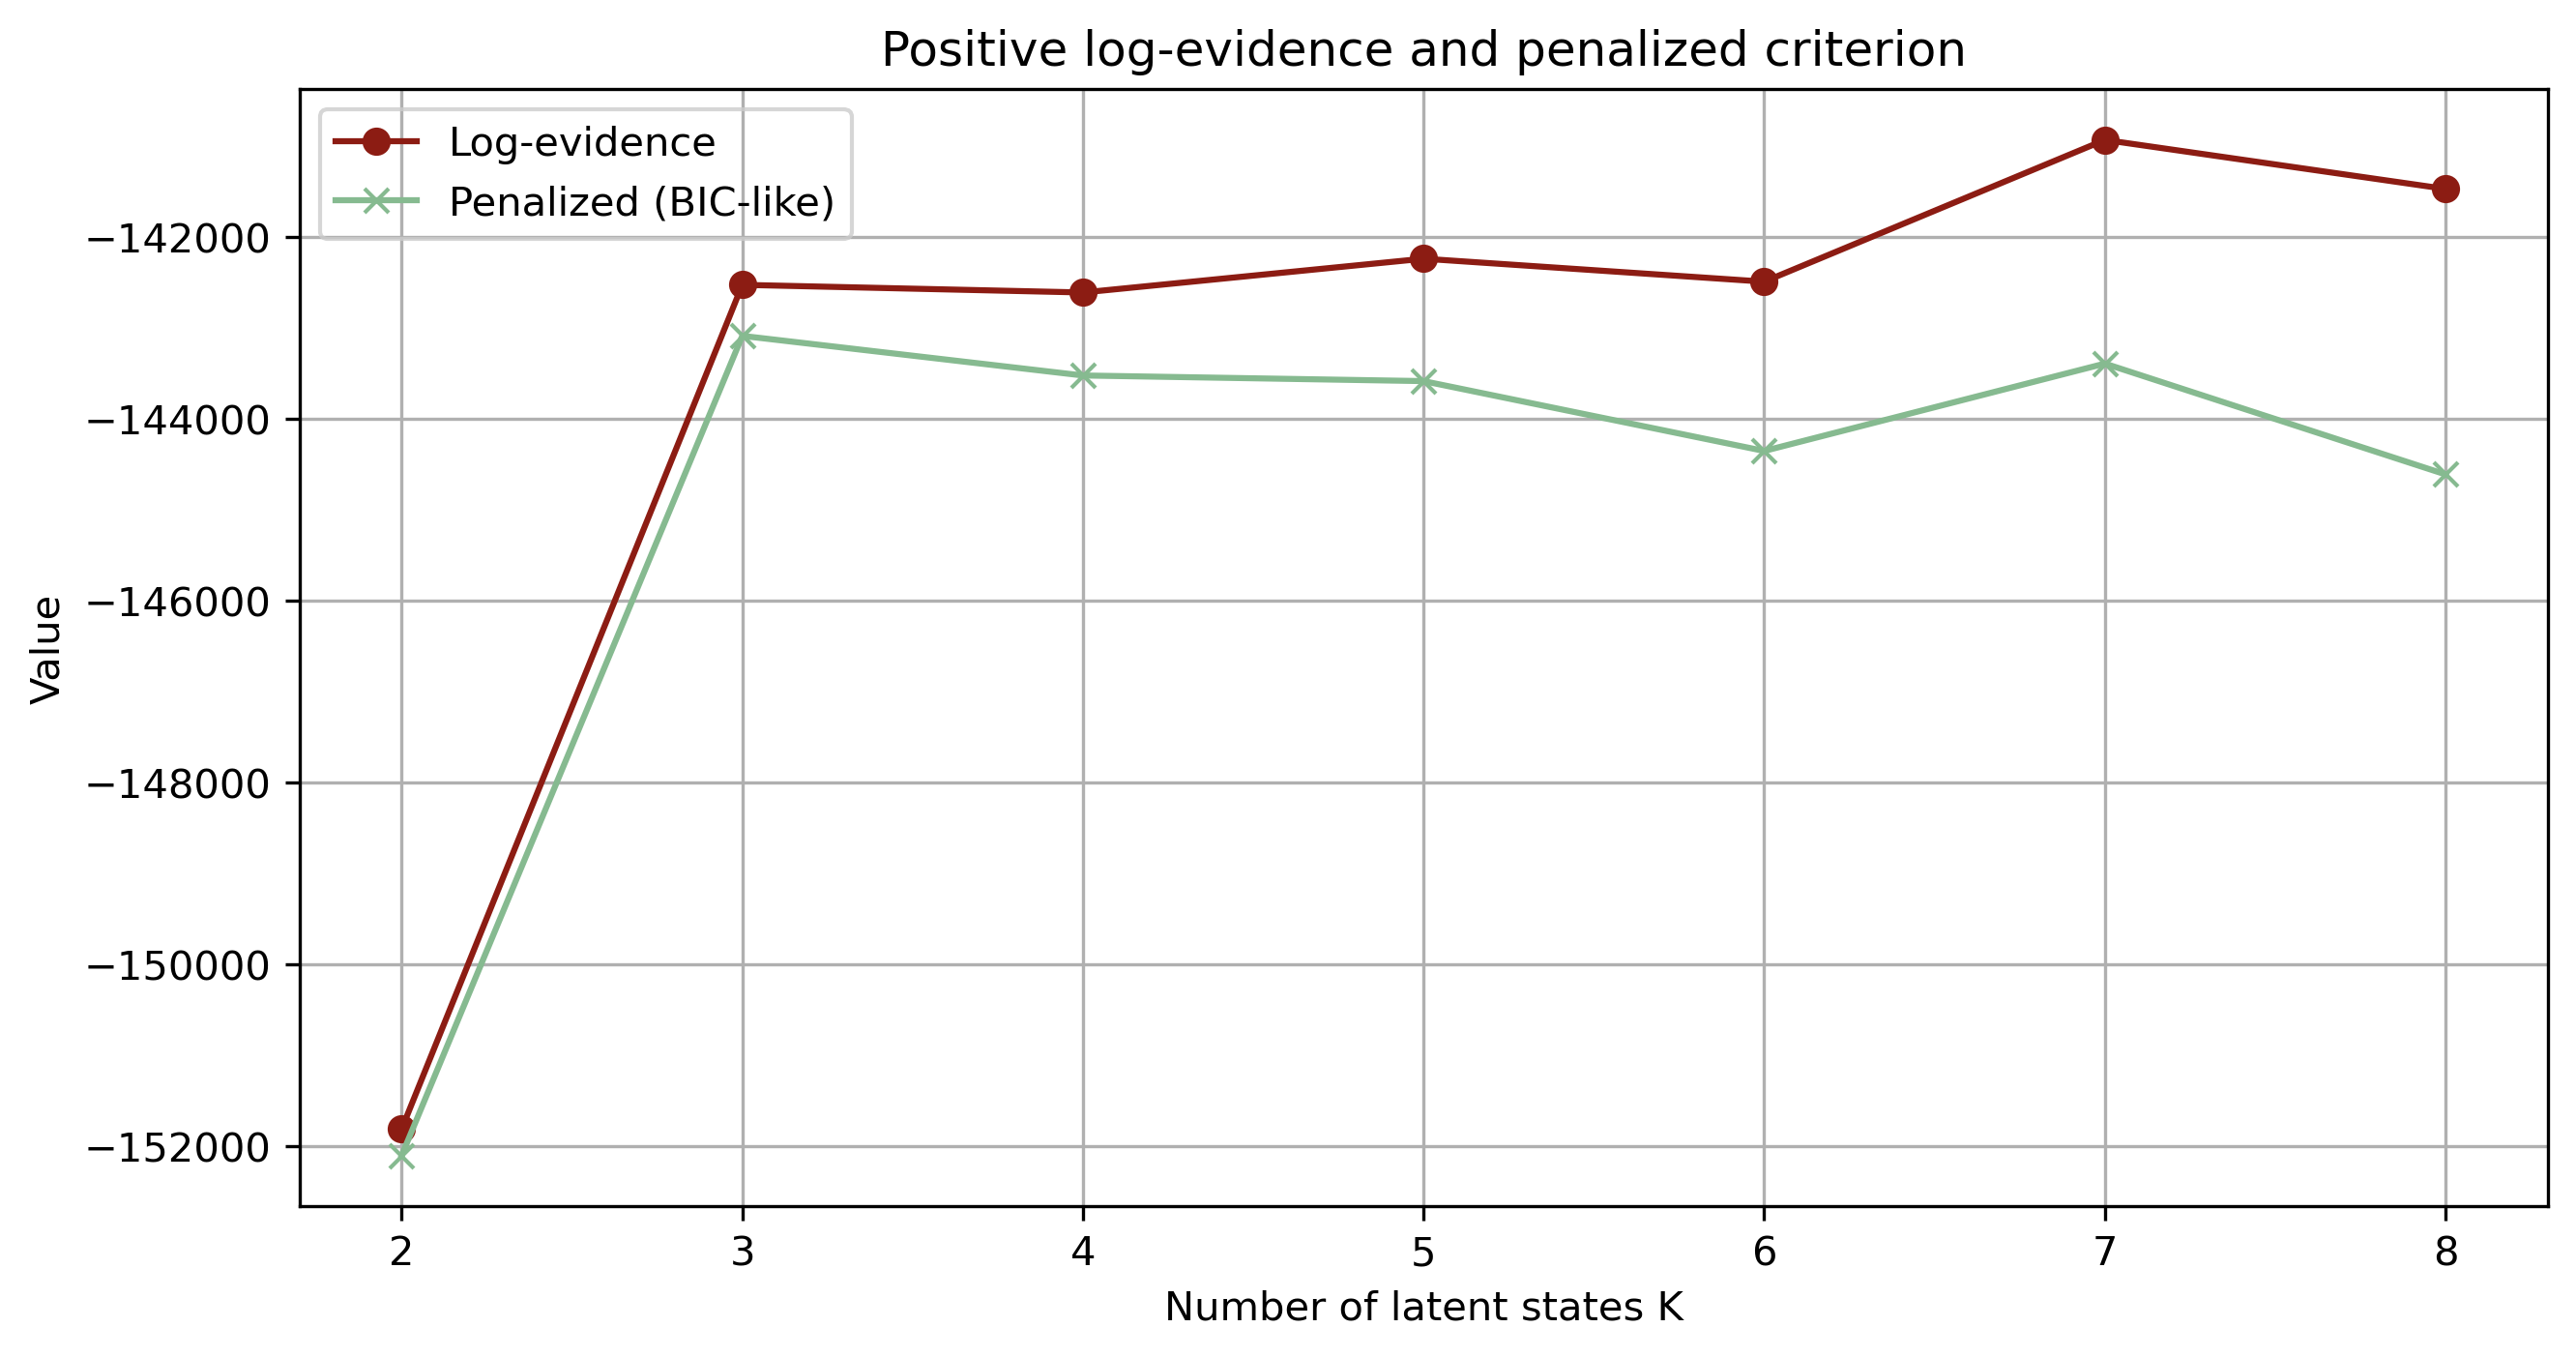
\includegraphics[keepaspectratio]{img/hmm/bic_plot.png}}

}

\caption{\label{fig-bic}Log-likelihood e BIC al variare del numero di
parametri}

\end{figure}%

\end{tcolorbox}

Dal punto di vista numerico, l'ottimizzazione è stata effettuata con
Adam a passo \(2\cdot 10^{-2}\), operando in \emph{full-batch} per ogni
step (tutte le sequenze in una singola \texttt{plate}), in quanto il
numero di osservazioni non era eccessivo. Il ciclo di addestramento ha
previsto 2000 step; l'ELBO decresce rapidamente nelle prime epoche per
poi stabilizzarsi. Al termine, i parametri vengono salvati nel
\texttt{ParamStore} per l'uso in produzione e per la riproducibilità
(modello in produzione ``prod'': \texttt{models/hmm\_glm\_full.pt};
modello per lo sviluppo ``dev'' per valutazioni su \emph{hold-out}:
\texttt{models/hmm\_glm\_train.pt}).

Per contenere i costi computazionali, si osservi che la complessità per
step è dell'ordine \(\mathcal{O}(N\,T\,K^2)\), dominata dalle
transizioni \(K\times K\) e dall'enumerazione; con \(K=3\) il training è
agevole anche su CPU. Tuttavia, il codice è costruito in modo da poter
essere girato anche su GPU Nvidia, attraverso l'utilizzo
dell'archittetura \texttt{cuda}, che permetterebbe lo sviluppo in
parallelo.

\begin{codelisting}

\caption{\label{lst-train}Allenamento del modello}

\centering{

\begin{Shaded}
\begin{Highlighting}[]
\NormalTok{pyro.clear\_param\_store()}
\NormalTok{svi }\OperatorTok{=}\NormalTok{ SVI(model, guide,}
\NormalTok{          Adam(\{}\StringTok{"lr"}\NormalTok{: }\FloatTok{2e{-}2}\NormalTok{\}),}
\NormalTok{          loss}\OperatorTok{=}\NormalTok{TraceEnum\_ELBO(max\_plate\_nesting}\OperatorTok{=}\DecValTok{1}\NormalTok{))}

\ControlFlowTok{for}\NormalTok{ step }\KeywordTok{in} \BuiltInTok{range}\NormalTok{(}\DecValTok{2000}\NormalTok{):}
\NormalTok{    loss }\OperatorTok{=}\NormalTok{ svi.step(obs\_torch,}
\NormalTok{                    cov\_init\_torch,}
\NormalTok{                    cov\_tran\_torch,}
\NormalTok{                    cov\_emiss\_torch)}
    \ControlFlowTok{if}\NormalTok{ step }\OperatorTok{\%} \DecValTok{200} \OperatorTok{==} \DecValTok{0}\NormalTok{:}
        \BuiltInTok{print}\NormalTok{(}\SpecialStringTok{f"}\SpecialCharTok{\{}\NormalTok{step}\SpecialCharTok{:4d\}}\SpecialStringTok{  ELBO = }\SpecialCharTok{\{}\NormalTok{loss}\SpecialCharTok{:,.0f\}}\SpecialStringTok{"}\NormalTok{)}

\NormalTok{param\_path }\OperatorTok{=}\NormalTok{ here(}\StringTok{"models/hmm\_glm\_full.pt"}\NormalTok{)}
\NormalTok{pyro.get\_param\_store().save(param\_path)}
\BuiltInTok{print}\NormalTok{(}\SpecialStringTok{f"ParamStore saved in: }\SpecialCharTok{\{}\NormalTok{param\_path}\SpecialCharTok{\}}\SpecialStringTok{"}\NormalTok{)}
\end{Highlighting}
\end{Shaded}

}

\end{codelisting}%

\section{Risultati}\label{risultati-3}

Poiché le tre componenti centrali dell'HMM-GLM sono la distribuzione
iniziale sugli stati, la matrice di transizione e l'emissione (GLM di
Poisson specifico di stato), presentiamo i risultati scomponendo
l'analisi lungo questi assi e distinguendo tra grandezze di
``popolazione'' (ottenute inserendo valori medi delle covariate) e
grandezze ``soggetto-specifiche'' (ottenute dalle covariate effettive di
ciascun donatore).

\begin{tcolorbox}[enhanced jigsaw, breakable, colframe=quarto-callout-note-color-frame, toprule=.15mm, colback=white, opacityback=0, rightrule=.15mm, bottomrule=.15mm, leftrule=.75mm, left=2mm, arc=.35mm]
\begin{minipage}[t]{5.5mm}
\textcolor{quarto-callout-note-color}{\faInfo}
\end{minipage}%
\begin{minipage}[t]{\textwidth - 5.5mm}

\vspace{-3mm}\textbf{Attenzione}\vspace{3mm}

A causa di diverse versioni del codice, nei riferimenti e nelle varie
rappresentazioni grafiche possono trovarsi etichette differenti per gli
stati. Adotteremo la seguente convenzione: lo stato 0 sarà lo stato del
non-donatore (\emph{Non-donor}); lo stato 1 del donatore saltuario
(\emph{Occasional donor}) e lo stato 2 del donatore frequente
(\emph{frequent donor}).

\end{minipage}%
\end{tcolorbox}

Per le probabilità iniziali si applica Equazione~\ref{eq-pi_initial}
(versione in termini matriciali di Equazione~\ref{eq-prob_iniziali}):
\begin{equation}\phantomsection\label{eq-pi_initial}{
\pi_n  =  \text{softmax}\!\big(\log \pi_{\text{base}} + x^\pi_n W_\pi^\top\big),
}\end{equation}

dove \(x^\pi_n\) sono le covariate del donatore \(n\). Un riassunto di
popolazione si ottiene sostituendo \(x^\pi_n\) con la media campionaria
delle covariate (plug-in) e calcolando la corrispondente \(\bar\pi\). Il
grafico in Figura~\ref{fig-init} mostra che la quota di donatori che, al
tempo iniziale, si colloca nello stato ``dormiente/non-donatore'' (stato
0) è molto elevata (circa 78\%). Le restanti masse si ripartiscono tra
stato 1 (saltuario, circa 19\%) e stato 2 (abituale, circa 3\%). Questo
esito è coerente con la struttura dei dati, che includono gli anni
precedenti alla prima donazione riempiti con zeri (completamento
longitudinale), e con la prior asimmetrica su \(\pi_{\text{base}}\) che
spezza la simmetria delle etichette e riflette l'alta prevalenza
iniziale dello stato 0.

La matrice di transizione media in Figura~\ref{fig-trans} evidenzia
forte persistenza di stato: la probabilità di permanenza sulla diagonale
è alta per tutti e tre gli stati (circa \(P(0\!\to\!0)\simeq 0{,}84\),
\(P(1\!\to\!1)\simeq 0{,}88\), \(P(2\!\to\!2)\simeq 0{,}87\)), mentre i
termini fuori diagonale sono tutti inferiori a circa 0,10. In termini
pratici, i passaggi tra profili comportamentali sono rari; ciò vale in
media e a parità di covariate, mentre a livello individuale le
probabilità di transizione vengono modulate dalle covariate
\(x^A_{n,t}\) (fasce d'età e indicatore COVID). Si osserva inoltre, a
livello di occupazione di stato nella popolazione, uno spostamento di
massa dagli stati meno attivi verso quelli più attivi nel 2020--2022,
coerente con l'effetto dell'indicatore COVID nelle transizioni
(Figura~\ref{fig-state_occupancy}).

\begin{figure}

\begin{minipage}{0.50\linewidth}

\centering{

\pandocbounded{
\includegraphics[keepaspectratio]{img/hmm/hmm_init_white.png}}

}

\subcaption{\label{fig-init}Occupazione degli stati iniziali}

\end{minipage}%
%
\begin{minipage}{0.50\linewidth}

\centering{

\pandocbounded{
\includegraphics[keepaspectratio]{img/hmm/hmm_trans_white.png}}

}

\subcaption{\label{fig-trans}Matrice di transizione}

\end{minipage}%
\newline
\begin{minipage}{\linewidth}

\centering{

\pandocbounded{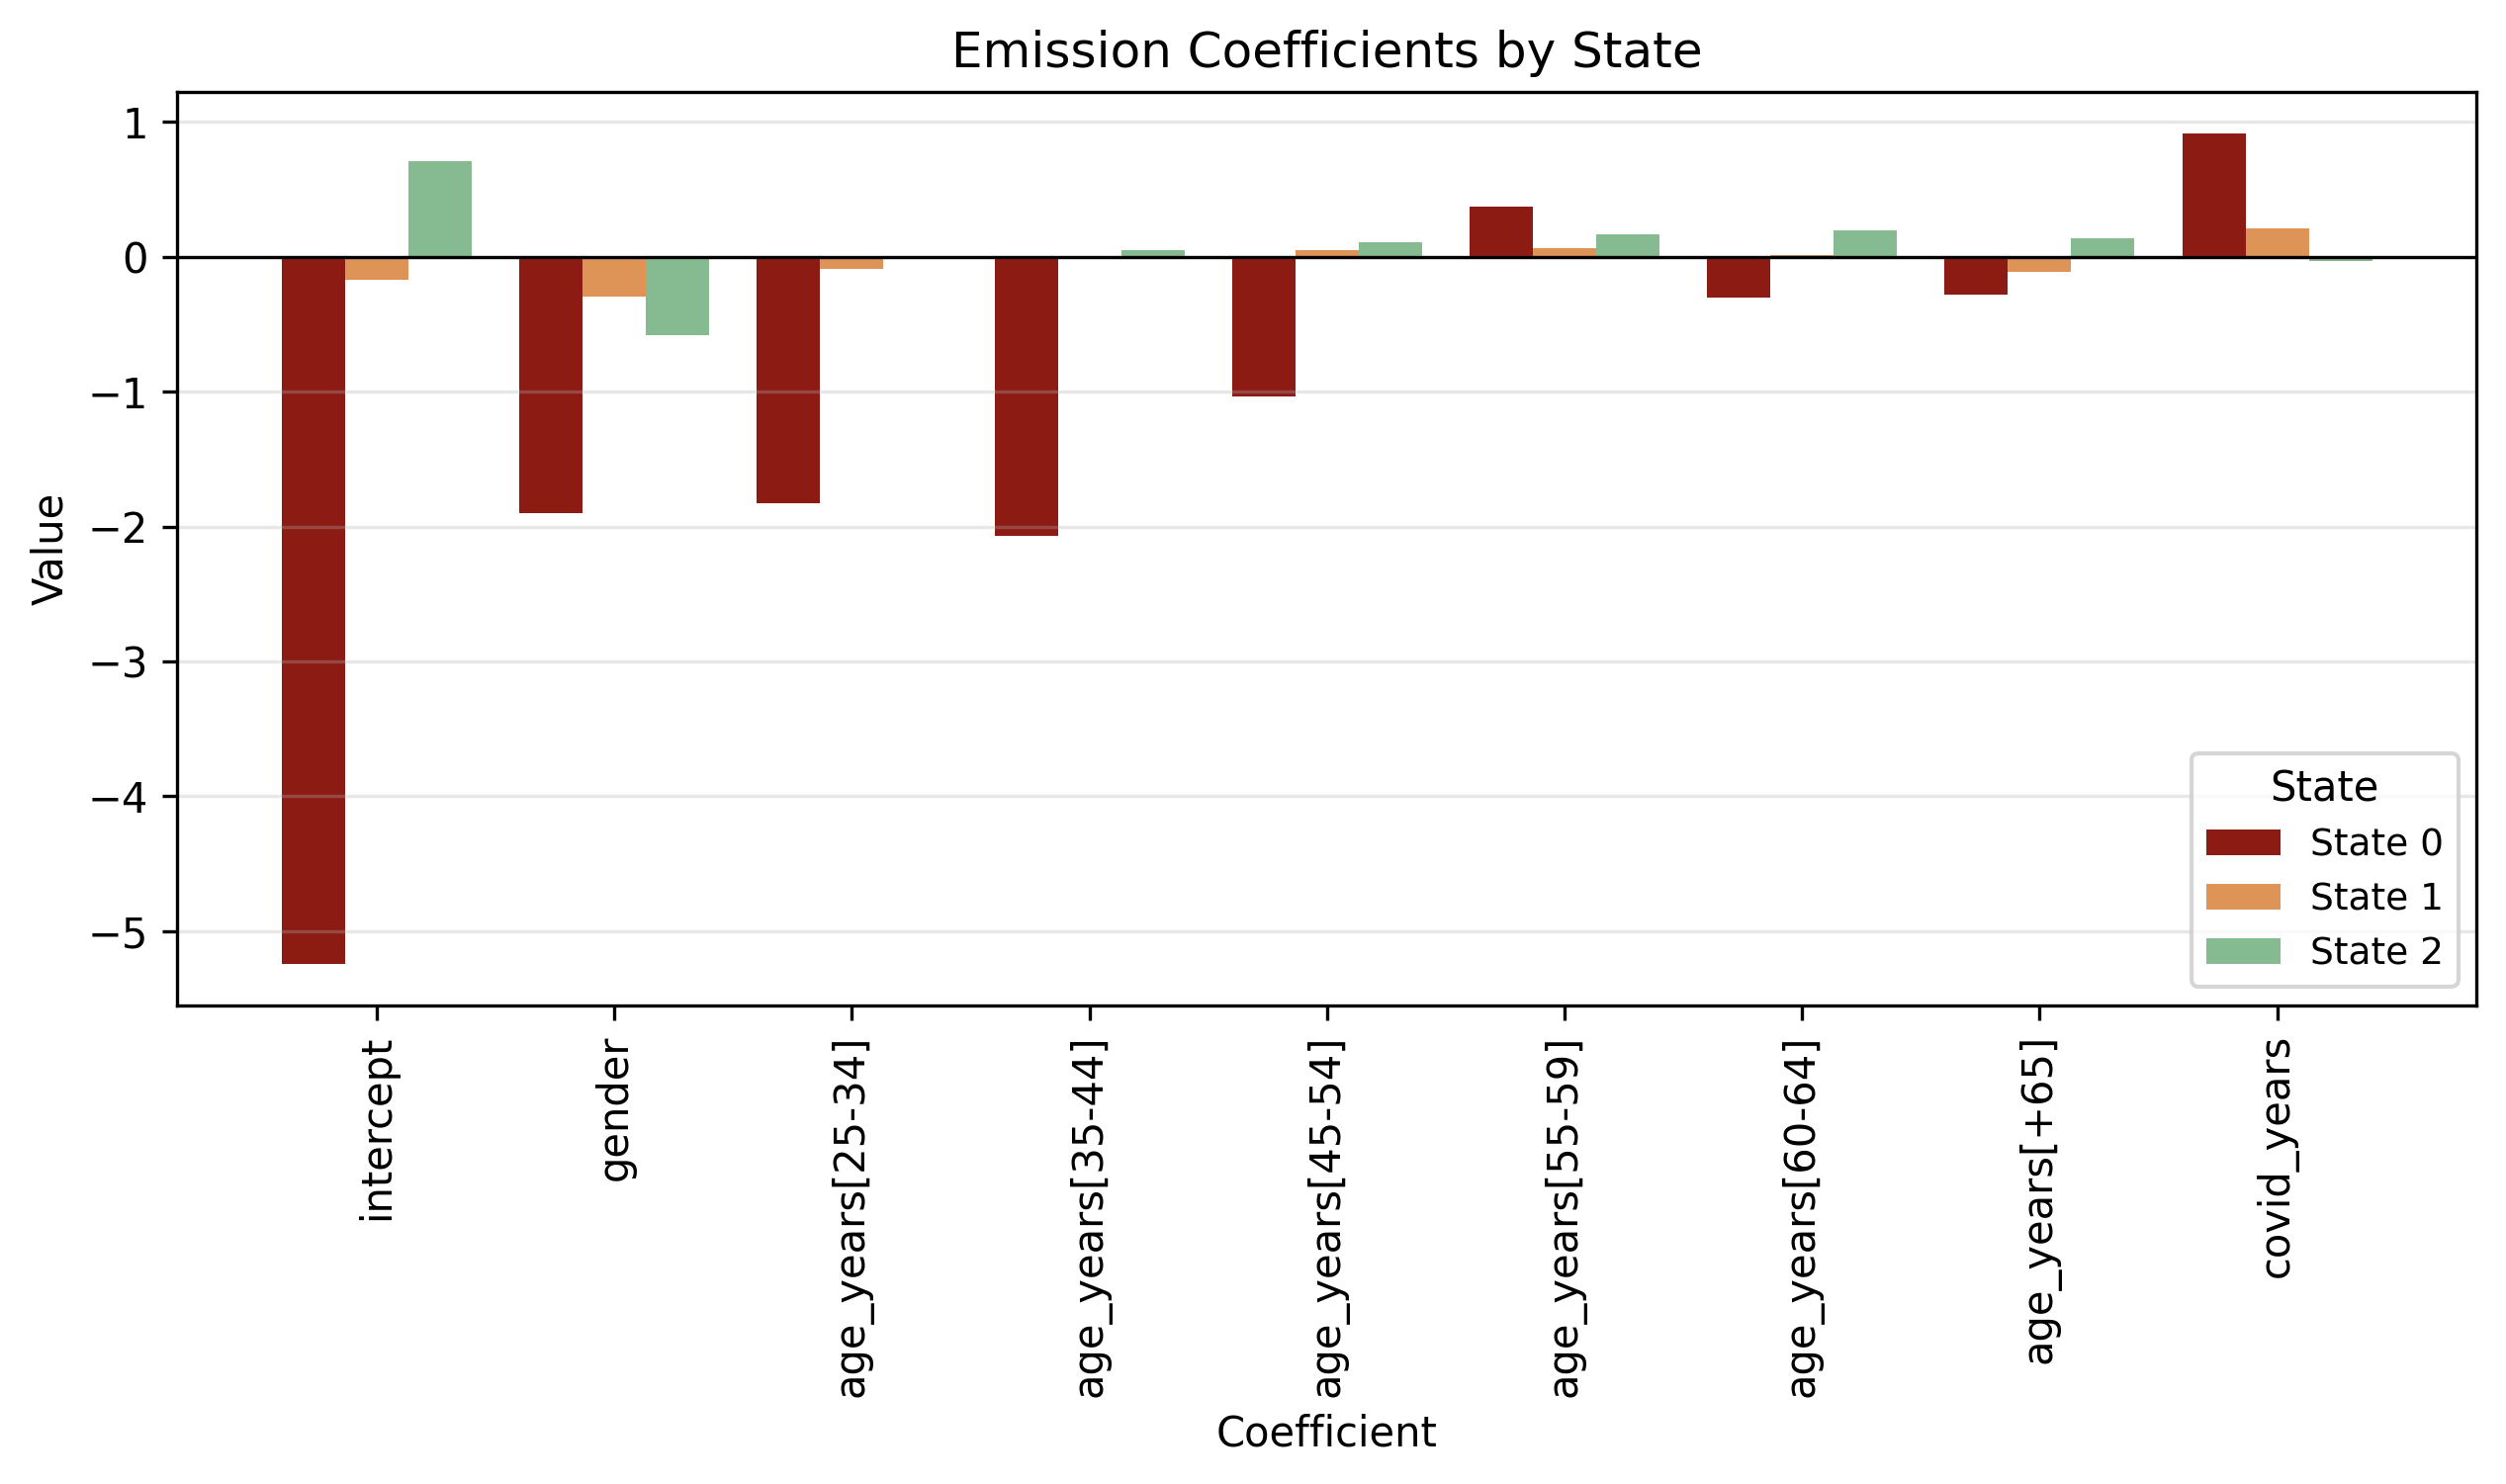
\includegraphics[keepaspectratio]{img/hmm/hmm_em_white.png}}

}

\subcaption{\label{fig-em}Coefficienti dei modelli GLM}

\end{minipage}%

\caption{\label{fig-hmm_results}Risultati principali del modello}

\end{figure}%

\subsection{\texorpdfstring{Coefficienti
\(\beta_{\text{em}}\)}{Coefficienti \textbackslash beta\_\{\textbackslash text\{em\}\}}}\label{coefficienti-beta_textem}

Per le emissioni non ha senso parlare di ``probabilità di donare \(x\)
nello stato \(k\)'' indipendentemente dalle covariate, perché nel nostro
HMM-GLM il tasso di Poisson dipende dallo stato e dalle covariate:
\(\log \lambda_{n,t,k} = x^{\text{em}}_{n,t}\cdot \beta_{\text{em},k}\).
La lettura più chiara è dunque in termini di coefficienti esponenziati,
che rappresentano effetti moltiplicativi sul valore atteso.

Il grafico in Figura~\ref{fig-em} e la tabella
Tabella~\ref{tbl-coeff_em} riportano, per ciascuno stato, l'intercetta
(donatore maschio, 18--24 anni, in periodo non COVID) e i fattori
moltiplicativi per genere, età e COVID. In particolare: l'intercetta
vale 0 nello stato 0 (dormiente), 0,84 nello stato 1 (saltuario) e 2,02
nello stato 2 (abituale). Il coefficiente ``gender'' (\textless1 in
tutti gli stati) implica, a parità di età e periodo, un tasso atteso
inferiore per le donne: ad esempio, nello stato 2 una donna 18--24 anni
in periodo non COVID ha \(2.02\times 0{,}56 \approx 1{,}14\) donazioni
attese (-44\% rispetto al maschio baseline). Gli effetti d'età sono
deboli nello stato 1 (fattori prossimi a 1) e crescenti nello stato 2:
per 55--59 anni il moltiplicatore è circa 1,18 e per 60--64 è circa 1,22
(in linea col profilo ``abituale'' più marcato nelle classi d'età
centrali-avanzate). L'indicatore COVID agisce in modo eterogeneo: è
\textgreater1 nello stato 1 (circa 1,24, ``boost'' relativo), circa 1
nello stato 2 (circa 0,97, lieve attenuazione/neutralità) e
\textgreater\textgreater1 nello stato 0 (circa 2,51), ma in quest'ultimo
caso l'aumento relativo non si traduce in un incremento assoluto
rilevante perché la base è approsimativamente 0.

\begin{longtable}[]{@{}
  >{\raggedright\arraybackslash}p{(\linewidth - 18\tabcolsep) * \real{0.1304}}
  >{\raggedleft\arraybackslash}p{(\linewidth - 18\tabcolsep) * \real{0.0942}}
  >{\raggedleft\arraybackslash}p{(\linewidth - 18\tabcolsep) * \real{0.0725}}
  >{\raggedleft\arraybackslash}p{(\linewidth - 18\tabcolsep) * \real{0.1087}}
  >{\raggedleft\arraybackslash}p{(\linewidth - 18\tabcolsep) * \real{0.1087}}
  >{\raggedleft\arraybackslash}p{(\linewidth - 18\tabcolsep) * \real{0.1087}}
  >{\raggedleft\arraybackslash}p{(\linewidth - 18\tabcolsep) * \real{0.1087}}
  >{\raggedleft\arraybackslash}p{(\linewidth - 18\tabcolsep) * \real{0.1087}}
  >{\raggedleft\arraybackslash}p{(\linewidth - 18\tabcolsep) * \real{0.0942}}
  >{\raggedleft\arraybackslash}p{(\linewidth - 18\tabcolsep) * \real{0.0652}}@{}}
\caption{Coeficcienti dei modelli GLM per stato elevati
all'esponenziale}\label{tbl-coeff_em}\tabularnewline
\toprule\noalign{}
\begin{minipage}[b]{\linewidth}\raggedright
\end{minipage} & \begin{minipage}[b]{\linewidth}\raggedleft
intercept
\end{minipage} & \begin{minipage}[b]{\linewidth}\raggedleft
gender
\end{minipage} & \begin{minipage}[b]{\linewidth}\raggedleft
age {[}25-34{]}
\end{minipage} & \begin{minipage}[b]{\linewidth}\raggedleft
age {[}35-44{]}
\end{minipage} & \begin{minipage}[b]{\linewidth}\raggedleft
age {[}45-54{]}
\end{minipage} & \begin{minipage}[b]{\linewidth}\raggedleft
age {[}55-59{]}
\end{minipage} & \begin{minipage}[b]{\linewidth}\raggedleft
age {[}60-64{]}
\end{minipage} & \begin{minipage}[b]{\linewidth}\raggedleft
age {[}+65{]}
\end{minipage} & \begin{minipage}[b]{\linewidth}\raggedleft
covid
\end{minipage} \\
\midrule\noalign{}
\endfirsthead
\toprule\noalign{}
\begin{minipage}[b]{\linewidth}\raggedright
\end{minipage} & \begin{minipage}[b]{\linewidth}\raggedleft
intercept
\end{minipage} & \begin{minipage}[b]{\linewidth}\raggedleft
gender
\end{minipage} & \begin{minipage}[b]{\linewidth}\raggedleft
age {[}25-34{]}
\end{minipage} & \begin{minipage}[b]{\linewidth}\raggedleft
age {[}35-44{]}
\end{minipage} & \begin{minipage}[b]{\linewidth}\raggedleft
age {[}45-54{]}
\end{minipage} & \begin{minipage}[b]{\linewidth}\raggedleft
age {[}55-59{]}
\end{minipage} & \begin{minipage}[b]{\linewidth}\raggedleft
age {[}60-64{]}
\end{minipage} & \begin{minipage}[b]{\linewidth}\raggedleft
age {[}+65{]}
\end{minipage} & \begin{minipage}[b]{\linewidth}\raggedleft
covid
\end{minipage} \\
\midrule\noalign{}
\endhead
\bottomrule\noalign{}
\endlastfoot
Non-donor & 0 & 0.13 & 0.16 & 0.11 & 0.53 & 10.35 & 0.59 & 0.69 &
2.15 \\
Occasional donor & 0.84 & 0.75 & 0.92 & 0.99 & 1.06 & 1.08 & 1.02 & 0.9
& 1.24 \\
Frequent donor & 2.02 & 0.56 & 1.01 & 1.05 & 1.11 & 1.18 & 1.22 & 1.15 &
0.97 \\
\end{longtable}

Nel complesso, le tre componenti del modello convergono verso un quadro
coerente: la maggior parte dei donatori inizia nello stato di bassa
attività, i profili sono altamente persistenti con rari passaggi tra
stati, i GLM per stato catturano differenze interpretabili per genere,
età e shock COVID, con un chiaro gradiente di intensità dallo stato 0
(quasi nullo) allo stato 2 (frequente). Per passare dalle letture di
popolazione a valutazioni soggetto-specifiche, nella sezione sul Viterbi
e sul filtraggio forward mostriamo come le distribuzioni sugli stati e
le previsioni one-step-ahead si ottengano combinando le \(A_{n,t}\)
condizionate alle covariate con i tassi \(\lambda_{n,t,k}\) dei GLM di
stato.

\subsection{\texorpdfstring{Coefficienti
\(W_\pi\)}{Coefficienti W\_\textbackslash pi}}\label{coefficienti-w_pi}

Osservando i coefficienti delle probabilità inziali \(W_\pi\), si nota
come la probabilità che un donatore inizi dallo stato 2 aumenti al
crescere dell'anno di nascita, mentre decresce la probabilità di inziare
dallo stato 0 (Figura~\ref{fig-pi_age}). Per il genere, invece, sarà più
probabile che una donatrice inizi dallo stato 0 che dallo stato 2,
mentre per lo stato 1 l'effetto è meno accentuato. Come visto nel
capitolo introduttivo, nelle analisi preliminari (vedi
Sezione~\ref{sec-analisi_preliminare}), osservando la tabella delle
donazioni per genere ed età (vedi
Tabella~\ref{tbl-donazioni_generarzioni}) si osservava come ci fosse un
forte incremento di donazioni da parte delle donatrici più giovani negli
ultimi anni. Ciò giustificherebbe i coefficienti presenti in
Figura~\ref{fig-coeff_pi}.

\begin{figure}

\begin{minipage}{0.50\linewidth}

\centering{

\pandocbounded{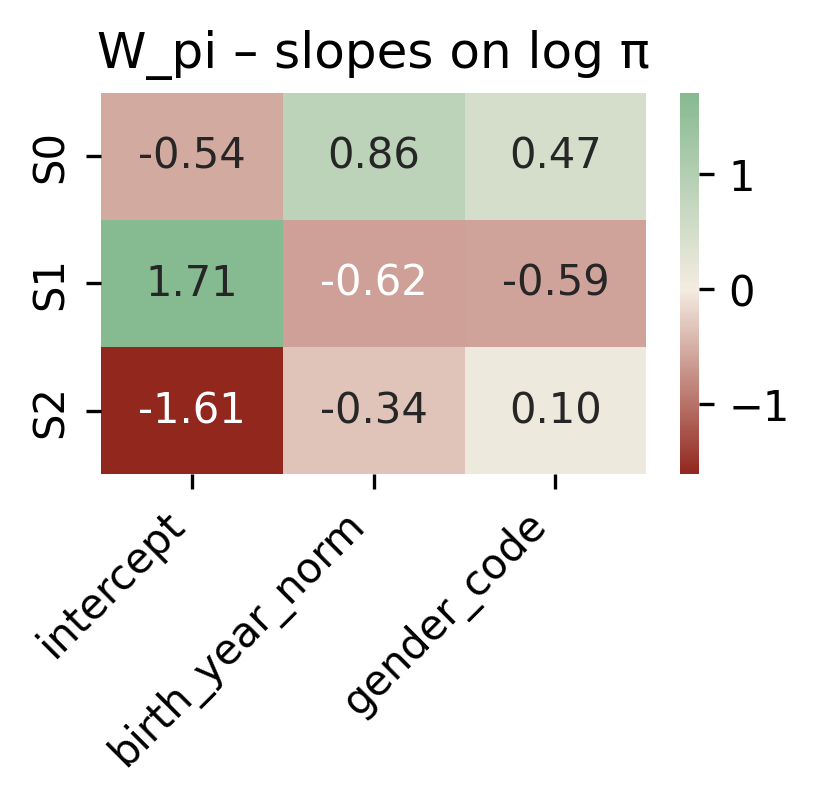
\includegraphics[keepaspectratio]{img/hmm/pi_coeff.png}}

}

\subcaption{\label{fig-coeff_pi}Coefficienti di \(W_\pi\)}

\end{minipage}%
%
\begin{minipage}{0.50\linewidth}

\centering{

\pandocbounded{
\includegraphics[keepaspectratio]{img/hmm/pi_age.png}}

}

\subcaption{\label{fig-pi_age}Distribuzione di probabilità per stato ed
anno di nascita}

\end{minipage}%

\caption{\label{fig-pi_results}Grafici sui valori dei coefficienti
\(W_\pi\)}

\end{figure}%

\subsection{\texorpdfstring{Coefficienti
\(W_A\)}{Coefficienti W\_A}}\label{sec-coeff_wa}

Dai coefficienti della matrice di transizione
Figura~\ref{fig-coeff_trans}, si possono trarre diverse osservazioni.

Partendo dalle fasce d'età, e in specifico dalla transizione
\(0 \to 0\), si può vedere come la probabilità di rimanere nello stato 0
decresca all'aumentare dell'età, ad eccezione della fascia +65. Infatti,
ricordiamo che il limite in Italia per donare sangue è di 65 anni, ad
eccezione dei donatori regolari, che è estesa a 70, previa consultazione
medica. Infatti aumenta la probabilità delle transizioni \(1 \to 0\) e
\(2 \to 1\) nella fascia +65.

Per quanto riguarda l'effetto covid, durante gli anni della pandemia la
probabilità delle transizioni \(0 \to 0\), \(1 \to 0\) e \(2 \to 0\)
erano minori, invece erano maggiori per le transizioni \(0 \to 1\) e
\(1 \to 1\). Si osserva anche che molti donatori frequenti, in quel
periodo, hanno ridotto il numero di donazioni (\(2 \to 1\)).

\begin{figure}

\centering{

\pandocbounded{
\includegraphics[keepaspectratio]{img/hmm/trans_coeff.png}}

}

\caption{\label{fig-coeff_trans}Coefficienti di \(W_A\)}

\end{figure}%

\section{Algoritmi e diagnostiche}\label{sec-viterbi}

\subsection{Viterbi con covariate}\label{viterbi-con-covariate}

Nel nostro HMM-GLM le tre componenti dipendono da covariate:

\begin{enumerate}
\def\labelenumi{\arabic{enumi}.}
\item
  la distribuzione iniziale \(\pi(x^\pi)\) tramite
  \(\,\text{softmax}(\log\pi_{\text{base}} + W_\pi x^\pi)\),
\item
  le transizioni \(A(x^A_t)\) tramite
  \(\,\text{softmax}(\log A_{\text{base}} + \langle W_A,\ x^A_t\rangle)\)
  e
\item
  l'emissione Poisson-GLM per stato \(k\) con
  \(\,\log\lambda_k(t)=x^{\text{em}}_t{}^\top\beta_{\text{em},k}\).
\end{enumerate}

A parametri fissati (plug-in), il percorso MAP \(z_{0:T}^*\) si ottiene
per programmazione dinamica, con un passo base e un passo iterativo.

\textbf{Inizializzazione:} tramite
l'Equazione~\ref{eq-viterbi_passo_base} si ricavano le probabilità per
stato al tempo 0. L'emissione (\(\log \Pr\bigl(y_0\mid z_0{=}k\bigr)\))
è la poisson con parametro
\(\lambda_k(0)=\exp\!\bigl(x^{\text{em}}_0{}^\top\beta_{\text{em},k}\bigr)\).
\begin{equation}\phantomsection\label{eq-viterbi_passo_base}{
\delta_0(k)=\log \pi_k(x^\pi) + \log \Pr\bigl(y_0\mid z_0{=}k\bigr),
}\end{equation}

\textbf{Ricorsione per \(t=1,\dots,T\):} in quest'altro caso
l'Equazione~\ref{eq-viterbi_passo_t} è data dal massimo della
probabilità di stare nello stato precedente, \(k\), sommato alla
probabilità di spostarsi al tempo \(t\) dallo stato \(k\) allo stato
\(j\). Successivamente viene sommata la log-probabilità di emissione.
\begin{equation}\phantomsection\label{eq-viterbi_passo_t}{
\delta_t(j)=\max_{k}\Big\{\delta_{t-1}(k) + \log A_{k\to j}\!\bigl(x^A_t\bigr)\Big\} + \log \Pr\bigl(y_t\mid z_t{=}j\bigr),
}\end{equation}

\textbf{Backtracking:} è più semplice del passo \emph{forward}, in
questo caso bisognerà cercare l'argomento che massimiza la funzione
\(\delta\).
\begin{equation}\phantomsection\label{eq-viterbi_back_tracking}{
z_T^*=\arg\max_j \delta_T(j),\qquad
z_{t-1}^*=\psi_t\!\bigl(z_t^*\bigr)\quad (t=T,\dots,1).
}\end{equation}

\subsubsection{Occupancy e Switch-rate}\label{occupancy-e-switch-rate}

Con l'algoritmo appena descritto, andiamo a calcolare per ogni donatore
nel nostro dataset la sue serie temporale attesa di stati latenti e
rappresentiamo in un grafico (vedi Figura~\ref{fig-state_occupancy}) la
loro distribuzione lungo gli anni. I risultati mostrano come lo stato 2,
ovvero dei donatori frequenti è abbastanza stabile e in leggero aumento.
Mentre, si nota come durante la pandemia ci sia stato un notevole
spostamento dallo stato 0 (non donatore) allo stato 1 (donatore
saltuario). Ciò è stato confermato nella sezione precedente
(Sezione~\ref{sec-coeff_wa}) dove attraverso il grafico dei coefficenti
della matrice di transizione \(W_A\) si osservava (vedi
Figura~\ref{fig-coeff_trans}) come la probabilità di passare dallo stato
0 a uno stato superiore fosse molto maggiore che in un periodo in
assenza della pandemia.

\begin{figure}

\centering{

\pandocbounded{
\includegraphics[keepaspectratio]{img/hmm/hmm_state_occupancy_white.png}}

}

\caption{\label{fig-state_occupancy}Occupazione degli stati per anno}

\end{figure}%

\subsection{Forward per log-likelihood}\label{sec-forward}

Data una serie di osservazioni, ovvero di donazioni e un set di
informazioni demografiche sull'individuo, il nostro scopo sarà quelllo
di prevedere il numero di donazioni all'anno successivo, dunque il suo
stato latente al tempo \(T+1\).

La forward recursion fornisce la log-verosimiglianza e la distribuzione
filtrata sugli stati, utile per la previsione one-step-ahead. Definendo
\(\alpha_t(j)=\Pr(z_t{=}j\mid y_{0:t})\) (fino a normalizzazione), si
ha:

\emph{Filtering} \begin{equation}\phantomsection\label{eq-filtering}{
\tilde\alpha_t(j)=\Pr(y_t\mid z_t{=}j)\sum_k \alpha_{t-1}(k)\,A_{k\to j}\!\bigl(x^A_t\bigr),
}\end{equation}

\begin{equation}\phantomsection\label{eq-filtering_norm}{
\alpha_t(j)=\frac{\tilde\alpha_t(j)}{\sum_h \tilde\alpha_t(h)}.
}\end{equation}

\emph{Log-verosimiglianza}

Indichiamo con \(c_t=\sum_h \tilde\alpha_t(h)\) il fattore di
normalizzazione; allora \(\log p(y_{0:T})=\sum_{t=0}^T \log c_t\),
oppure, equivalmente, \(\log p(y_{0:T})=\log\!\sum_j \alpha_T(j)\) se si
lavora interamente in log-spazio senza rinormalizzazioni intermedie.

Previsione one-step-ahead (mixture predittiva). Condizionando su
\(\alpha_T\) e propagando con la transizione covariata al tempo
\(T\!+\!1\),
\begin{equation}\phantomsection\label{eq-log_likelihood_osa}{
p_{T+1}(j)=\sum_k \alpha_T(k)\,A_{k\to j}\!\bigl(x^A_{T+1}\bigr),
}\end{equation}

\begin{equation}\phantomsection\label{eq-one_step_ahead_expected}{
\mathbb{E}[\,y_{T+1}\mid y_{0:T}\,]=\sum_{j=1}^K p_{T+1}(j)\,\lambda_j(T{+}1),
}\end{equation}

dove
\(\lambda_j(T{+}1)=\exp\bigl(x^{\text{em}}_{T+1}{}^\top \beta_{\text{em},j}\bigr)\).
Poiché la predittiva è una mistura di Poisson, sono immediati anche
\(\,\Pr(y_{T+1}{=}0)=\sum_j p_{T+1}(j)\exp\bigl(-\lambda_j(T{+}1)\bigr)\)
e \(\,\Pr(y_{T+1}{>}0)=1-\Pr(y_{T+1}{=}0)\). (Degirmenci (2014))

\subsubsection{Predizioni}\label{predizioni}

Una volta montato l'algoritmo in Python, sarà necessario dare in input
gli argomenti necessari al modello che sono: \texttt{birth\_year},
\texttt{gender} e \texttt{history\_counts} che contiene il numero di
donazioni per anno osservate finora. La funzione restituirà, attraverso
l'algoritmo appena descritto, la probabilità di appartenere allo stato
\(k\) al tempo \(T+1\) (vedi Tabella~\ref{tbl-next_prob}) ma anche al
tempo \(1, \dots, T\) (vedi Tabella~\ref{tbl-path}), il valore atteso
del prossimo numero di donazioni e la sua distribuzione (vedi
Tabella~\ref{tbl-donazioni_future}).

\begin{tcolorbox}[enhanced jigsaw, breakable, colframe=quarto-callout-note-color-frame, toprule=.15mm, title=\textcolor{quarto-callout-note-color}{\faInfo}\hspace{0.5em}{Nota}, arc=.35mm, colback=white, bottomrule=.15mm, bottomtitle=1mm, colbacktitle=quarto-callout-note-color!10!white, toptitle=1mm, titlerule=0mm, opacityback=0, rightrule=.15mm, opacitybacktitle=0.6, leftrule=.75mm, left=2mm, coltitle=black]

Le osservazioni vanno dal 2009 al 2023. Tuttavia, per poter far un
confronto tra la predizione e il valore reale, la serie storica è stata
troncata al tempo \(T\). Questo dimostra anche una flessibilità nel
modello, che non necessità un numero fisso di osservazioni temporali.

\end{tcolorbox}

\begin{longtable}[]{@{}
  >{\raggedright\arraybackslash}p{(\linewidth - 28\tabcolsep) * \real{0.2821}}
  >{\raggedright\arraybackslash}p{(\linewidth - 28\tabcolsep) * \real{0.0513}}
  >{\raggedright\arraybackslash}p{(\linewidth - 28\tabcolsep) * \real{0.0513}}
  >{\raggedright\arraybackslash}p{(\linewidth - 28\tabcolsep) * \real{0.0513}}
  >{\raggedright\arraybackslash}p{(\linewidth - 28\tabcolsep) * \real{0.0513}}
  >{\raggedright\arraybackslash}p{(\linewidth - 28\tabcolsep) * \real{0.0513}}
  >{\raggedright\arraybackslash}p{(\linewidth - 28\tabcolsep) * \real{0.0513}}
  >{\raggedright\arraybackslash}p{(\linewidth - 28\tabcolsep) * \real{0.0513}}
  >{\raggedright\arraybackslash}p{(\linewidth - 28\tabcolsep) * \real{0.0513}}
  >{\raggedright\arraybackslash}p{(\linewidth - 28\tabcolsep) * \real{0.0513}}
  >{\raggedright\arraybackslash}p{(\linewidth - 28\tabcolsep) * \real{0.0513}}
  >{\raggedright\arraybackslash}p{(\linewidth - 28\tabcolsep) * \real{0.0513}}
  >{\raggedright\arraybackslash}p{(\linewidth - 28\tabcolsep) * \real{0.0513}}
  >{\raggedright\arraybackslash}p{(\linewidth - 28\tabcolsep) * \real{0.0513}}
  >{\raggedright\arraybackslash}p{(\linewidth - 28\tabcolsep) * \real{0.0513}}@{}}
\caption{Esempio di predizione dello stato latente per anno in base al
numero di donazioni effettuate}\label{tbl-path}\tabularnewline
\toprule\noalign{}
\begin{minipage}[b]{\linewidth}\raggedright
Years (20XX)
\end{minipage} & \begin{minipage}[b]{\linewidth}\raggedright
09
\end{minipage} & \begin{minipage}[b]{\linewidth}\raggedright
10
\end{minipage} & \begin{minipage}[b]{\linewidth}\raggedright
11
\end{minipage} & \begin{minipage}[b]{\linewidth}\raggedright
12
\end{minipage} & \begin{minipage}[b]{\linewidth}\raggedright
13
\end{minipage} & \begin{minipage}[b]{\linewidth}\raggedright
14
\end{minipage} & \begin{minipage}[b]{\linewidth}\raggedright
15
\end{minipage} & \begin{minipage}[b]{\linewidth}\raggedright
16
\end{minipage} & \begin{minipage}[b]{\linewidth}\raggedright
17
\end{minipage} & \begin{minipage}[b]{\linewidth}\raggedright
18
\end{minipage} & \begin{minipage}[b]{\linewidth}\raggedright
19
\end{minipage} & \begin{minipage}[b]{\linewidth}\raggedright
20
\end{minipage} & \begin{minipage}[b]{\linewidth}\raggedright
21
\end{minipage} & \begin{minipage}[b]{\linewidth}\raggedright
22
\end{minipage} \\
\midrule\noalign{}
\endfirsthead
\toprule\noalign{}
\begin{minipage}[b]{\linewidth}\raggedright
Years (20XX)
\end{minipage} & \begin{minipage}[b]{\linewidth}\raggedright
09
\end{minipage} & \begin{minipage}[b]{\linewidth}\raggedright
10
\end{minipage} & \begin{minipage}[b]{\linewidth}\raggedright
11
\end{minipage} & \begin{minipage}[b]{\linewidth}\raggedright
12
\end{minipage} & \begin{minipage}[b]{\linewidth}\raggedright
13
\end{minipage} & \begin{minipage}[b]{\linewidth}\raggedright
14
\end{minipage} & \begin{minipage}[b]{\linewidth}\raggedright
15
\end{minipage} & \begin{minipage}[b]{\linewidth}\raggedright
16
\end{minipage} & \begin{minipage}[b]{\linewidth}\raggedright
17
\end{minipage} & \begin{minipage}[b]{\linewidth}\raggedright
18
\end{minipage} & \begin{minipage}[b]{\linewidth}\raggedright
19
\end{minipage} & \begin{minipage}[b]{\linewidth}\raggedright
20
\end{minipage} & \begin{minipage}[b]{\linewidth}\raggedright
21
\end{minipage} & \begin{minipage}[b]{\linewidth}\raggedright
22
\end{minipage} \\
\midrule\noalign{}
\endhead
\bottomrule\noalign{}
\endlastfoot
Counts & 0 & 0 & 0 & 3 & 4 & 3 & 4 & 3 & 4 & 3 & 2 & 2 & 2 & 3 \\
Viterbi st. & 0 & 0 & 0 & 2 & 2 & 2 & 2 & 2 & 2 & 2 & 2 & 2 & 2 & 2 \\
\end{longtable}

\begin{longtable}[]{@{}llll@{}}
\caption{Probabilità di appartenere allo stato \(k\) in
\(T+1\)}\label{tbl-next_prob}\tabularnewline
\toprule\noalign{}
State & 0 & 1 & 2 \\
\midrule\noalign{}
\endfirsthead
\toprule\noalign{}
State & 0 & 1 & 2 \\
\midrule\noalign{}
\endhead
\bottomrule\noalign{}
\endlastfoot
Next-state probabilities: & 0.005 & 0.125 & 0.870 \\
\end{longtable}

\begin{longtable}[]{@{}llllll@{}}
\caption{Probabilità delle donazioni
future}\label{tbl-donazioni_future}\tabularnewline
\toprule\noalign{}
\# donations & 0 & 1 & 2 & 3 & 4 \\
\midrule\noalign{}
\endfirsthead
\toprule\noalign{}
\# donations & 0 & 1 & 2 & 3 & 4 \\
\midrule\noalign{}
\endhead
\bottomrule\noalign{}
\endlastfoot
Probability & 0.175 & 0.275 & 0.252 & 0.164 & 0.131 \\
Expected next donations: & 1.871 & & & & \\
Prob donate next: & 0.824 & & & & \\
\end{longtable}

In Figura~\ref{fig-predizioni} si possono vedere degli esempi su
donatori che seguono traiettorie ben distinte tra loro. Il modello è
capace di seguire le loro traiettorie e adattarsi in eventuali cambi di
comportamento del donatore. In Figura~\ref{fig-8005}, il modello è
\emph{dormiente} fino alla sua prima donazione per poi assegnare al
donatore lo stato 2, ovvero di donatore frequente. In
Figura~\ref{fig-2002}, invece, il donatore inzia da uno stato 2 per poi
passare nel tempo a un calo nel numero di donazioni annue, ed il suo
stato mutua da 2 a 1. Alla fine di ciascun grafico è presente il numero
di donazioni predetto dal modello e il numero di donazioni
effettivamente effettuate all'anno \(T+1\). Il colore del triangolo
rappresenta lo stato più probabile all'anno successivo.

\begin{figure}

\begin{minipage}{0.50\linewidth}

\centering{

\pandocbounded{
\includegraphics[keepaspectratio]{img/hmm/predict_2002.png}}

}

\subcaption{\label{fig-2002}Contrazione delle donazioni}

\end{minipage}%
%
\begin{minipage}{0.50\linewidth}

\centering{

\pandocbounded{
\includegraphics[keepaspectratio]{img/hmm/predict_3012.png}}

}

\subcaption{\label{fig-3012}Donatore recente}

\end{minipage}%
\newline
\begin{minipage}{0.50\linewidth}

\centering{

\pandocbounded{
\includegraphics[keepaspectratio]{img/hmm/predict_4011.png}}

}

\subcaption{\label{fig-4011}Donatore frequente}

\end{minipage}%
%
\begin{minipage}{0.50\linewidth}

\centering{

\pandocbounded{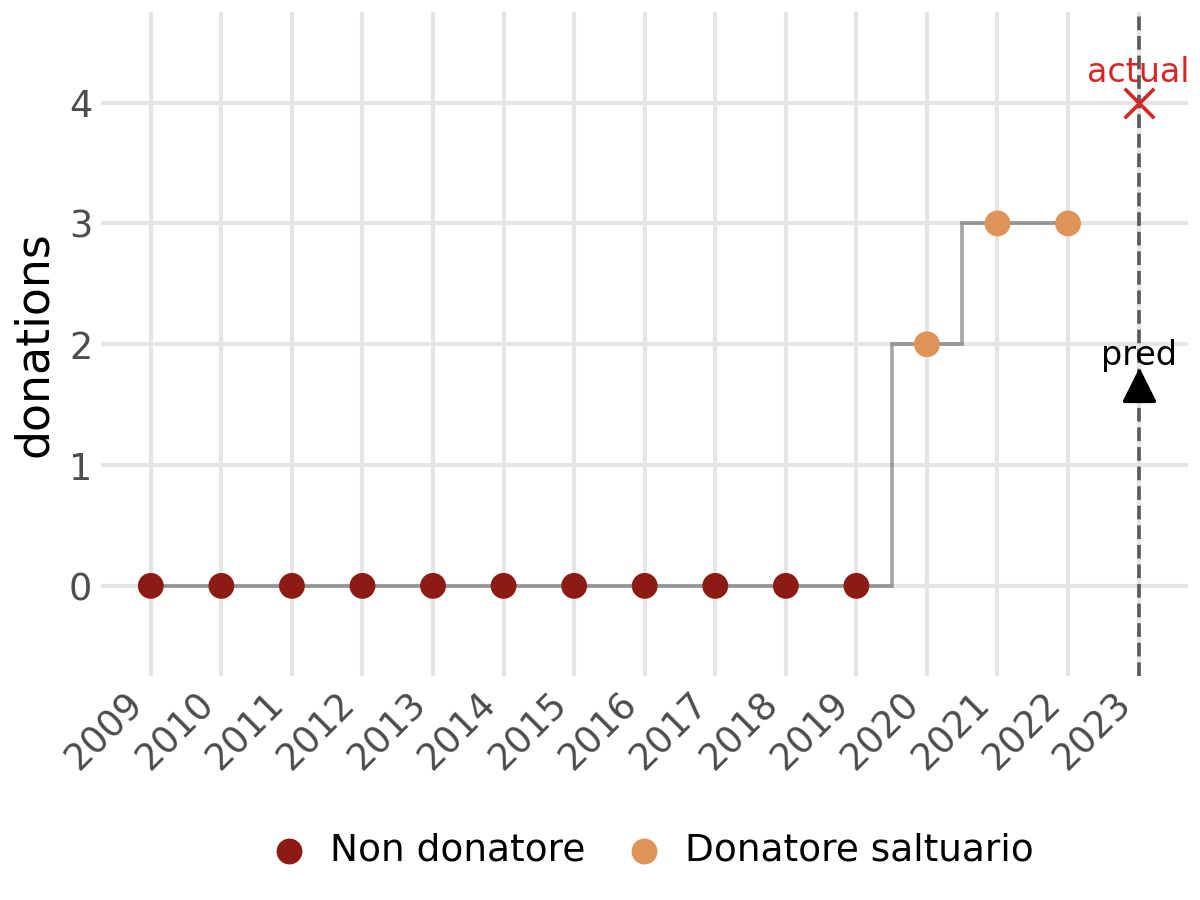
\includegraphics[keepaspectratio]{img/hmm/predict_8005.png}}

}

\subcaption{\label{fig-8005}Donatore recente}

\end{minipage}%

\caption{\label{fig-predizioni}Predizione del numero di donazioni per
diversi profili di donatore}

\end{figure}%

\subsection{Calibrazione e confronto con
GLM}\label{calibrazione-e-confronto-con-glm}

Per valutare la capacità predittiva in senso comparativo abbiamo
utilizzato come benchmark un GLM di Poisson ``vanilla'' senza stati
latenti, alimentato con le stesse covariate usate nelle emissioni
(intercetta, genere, fasce d'età, indicatore COVID). In questo modo
l'incremento di performance è attribuibile alla componente latente
(personalizzazione per stato e dinamica via transizioni).

Come descritto nella sezione sull'allenamento
(Sezione~\ref{sec-allenamento}), la valutazione è stata condotta su uno
split train/test 90/10 stratificato per genere e fascia d'età al tempo
iniziale (seed fisso), così da mitigare bias e overfitting e garantire
comparabilità.

\subsubsection{Metrica}\label{metrica}

Come metrica principale è stata usata l'\emph{accuracy} su conteggi
discreti è definita come
\begin{equation}\phantomsection\label{eq-accuracy}{
\mathrm{Accuracy} = \frac{1}{N}\sum_{n=1}^N \mathbf{I}\!\big\{\operatorname{round}(\hat y_n) = y_n\big\},
}\end{equation}

dove le predizioni sono arrotondate all'intero più vicino e ricondotte
all'intervallo consentito \([0,4]\) prima del confronto. La stessa
convenzione di arrotondamento è stata applicata a entrambi i modelli.

\subsubsection{Predizione HMM-GLM}\label{predizione-hmm-glm}

Per il punto di previsione in \(T{+}1\) usiamo due metodi distinti: in
un caso considereremo la mistura sugli stati come fatto nel capitolo
precedente (Sezione~\ref{sec-forward}); nell'altro selezioneremo solo lo
stato più probabile in \(T{+}1\), \(j^\star = \arg\max_j\, p_{T+1}(j),\)
e applicheremo il GLM di quello stato:
\begin{equation}\phantomsection\label{eq-pred_glm}{
\widehat y_{T+1} = \operatorname{round}\!\big(\exp(x^{\mathrm{em}}_{T+1}{}^\top \beta_{\mathrm{em},\,j^\star})\big),
}\end{equation}

con successivo clipping in \([0,4]\).

\subsubsection{Risultati}\label{risultati-4}

L'HMM-GLM ottiene un'accuracy superiore al GLM (42.24\% vs 27.48\%; vedi
figura Figura~\ref{fig-accuracy}), ottenendo dunque una predizione
migliore basata solamente sul numero di unità predette correttamente.
Tuttavia, sul livello medio, il GLM è più vicino all'osservato mentre
l'HMM-GLM tende a sottostimare.

\begin{figure}

\centering{

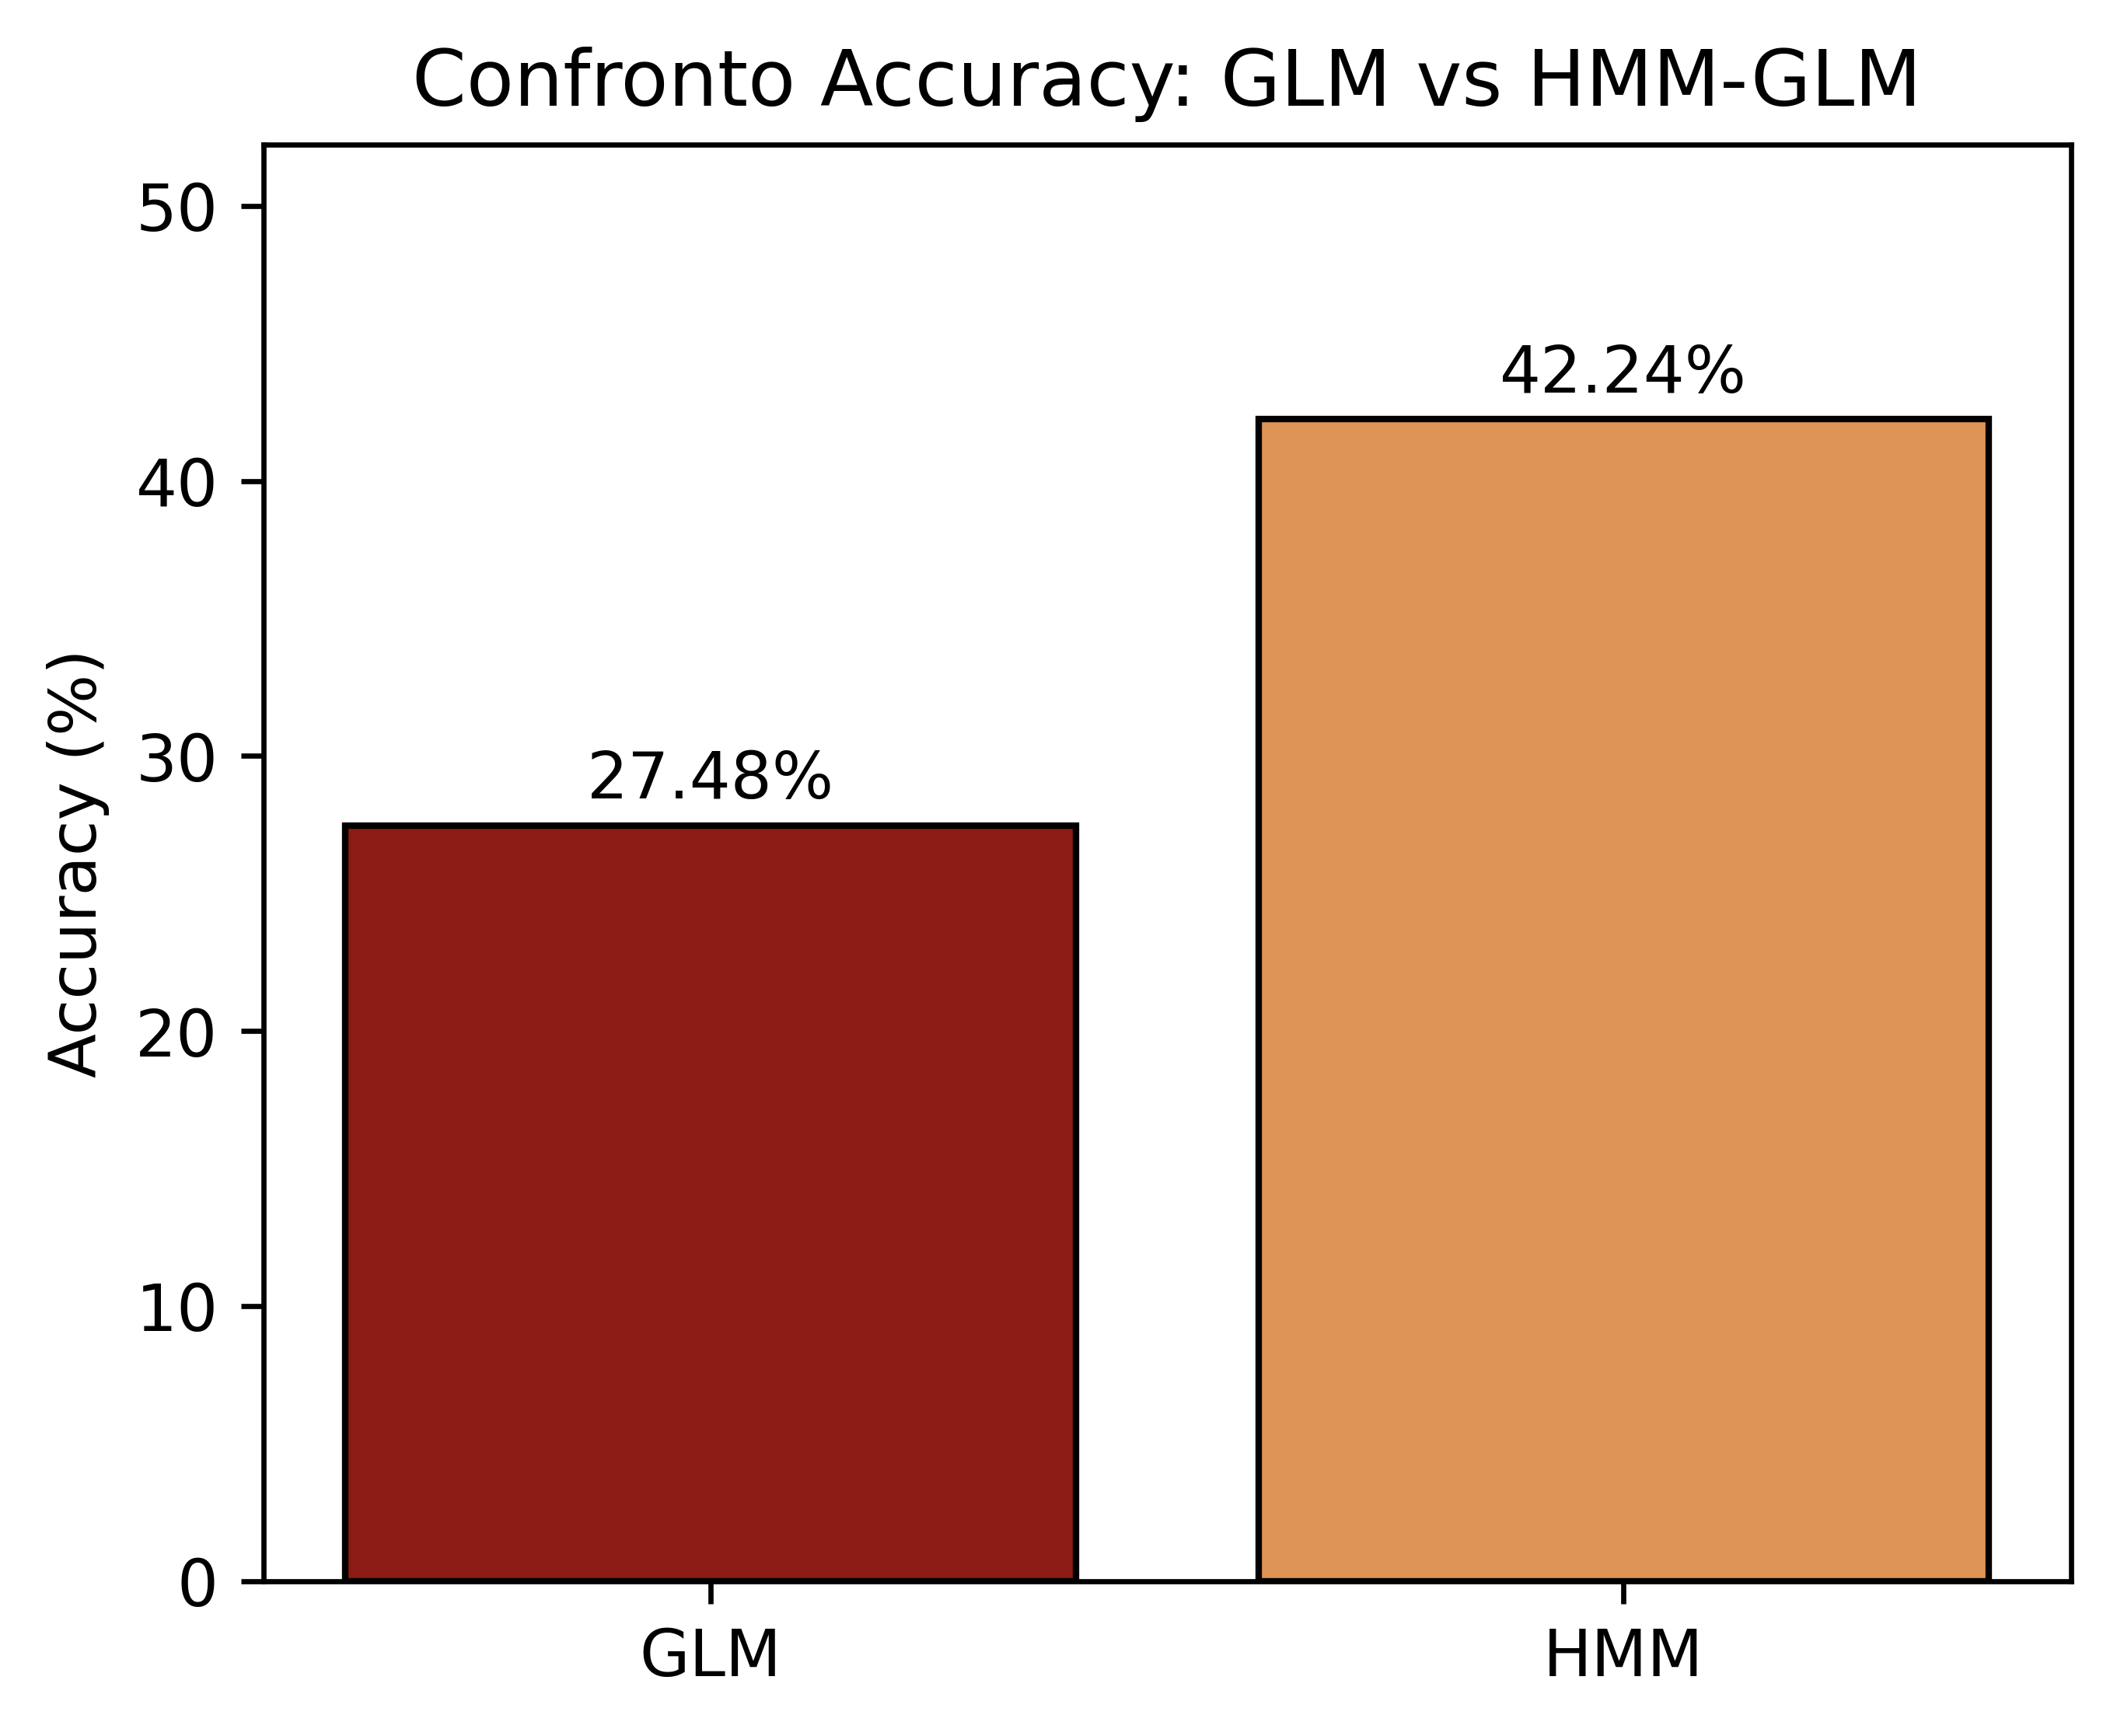
\includegraphics[width=0.5\linewidth,height=\textheight,keepaspectratio]{img/hmm/accuracy.png}

}

\caption{\label{fig-accuracy}Accuracy dei modelli}

\end{figure}%

\subsubsection{Analisi degli errori}\label{analisi-degli-errori}

Le mappe di calore in Figura~\ref{fig-errori} mostrano la distribuzione
percentuale degli errori arrotondati \((\hat y - y)\). Per l'HMM-GLM
predetto sul solo stato più probabile (Figura~\ref{fig-err_hmm_os})
emerge una forte massa in 0 (predizione esatta) e, a seguire, in -1 e -2
(sottostima), mostrando una forte assimetria degli errori; per il
modello HMM-GLM che, invece, considera tutti possibili stati futuri e
calcola una predizione pesata su di essi, si ottiene una accuracy
leggermente minore ma una simmetria maggiore e l'intervallo \([-1, 1]\)
contiene all'incirca l'80\% delle predizioni; per il GLM
(Figura~\ref{fig-err_glm}) la maggior parte degli errori è tra -1 e 1
con dispersione più simmetrica. Ciò è coerente con il fatto che
l'HMM-GLM ``aggancia'' meglio le categorie discrete grazie allo stato
selezionato, mentre il GLM media meglio il livello.

\begin{figure}

\begin{minipage}{\linewidth}

\centering{

\pandocbounded{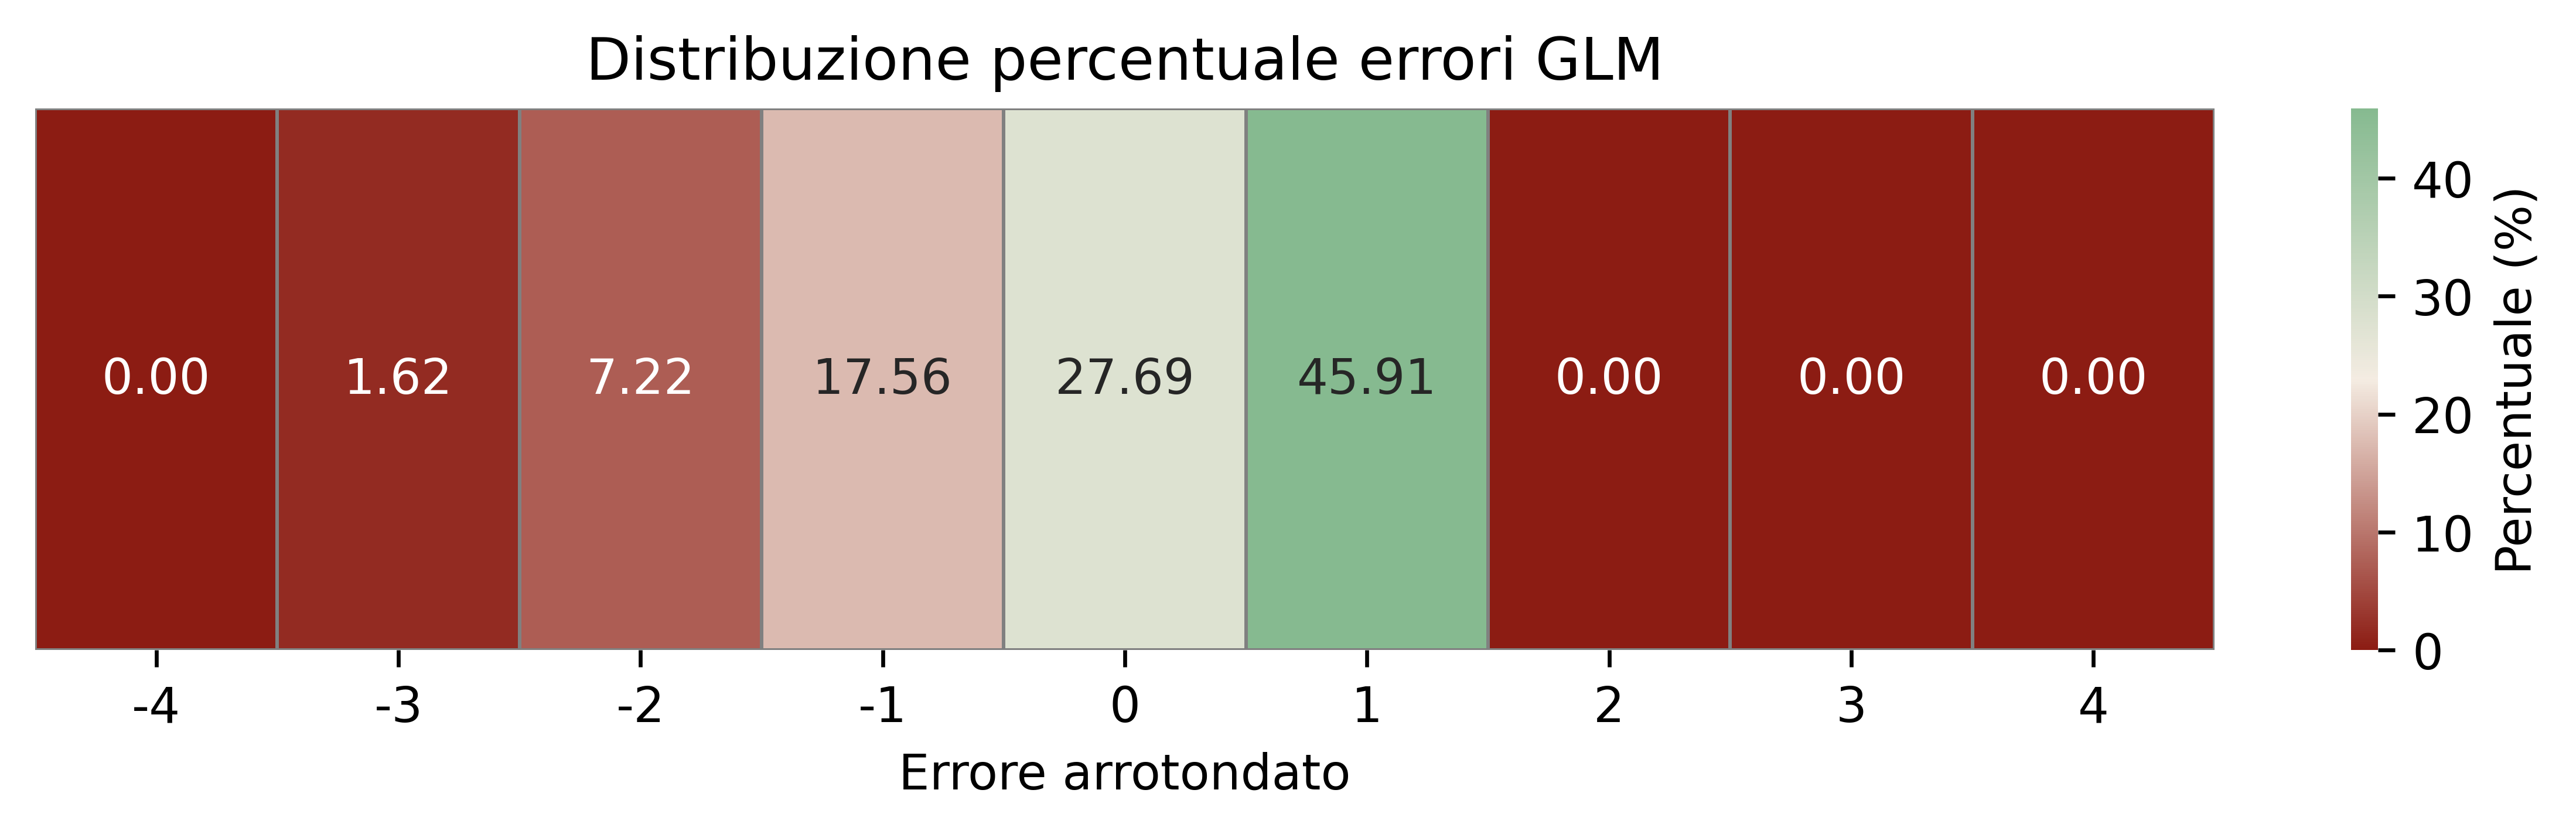
\includegraphics[keepaspectratio]{img/hmm/glm_error.png}}

}

\subcaption{\label{fig-err_glm}Errori del GLM}

\end{minipage}%
\newline
\begin{minipage}{\linewidth}

\centering{

\pandocbounded{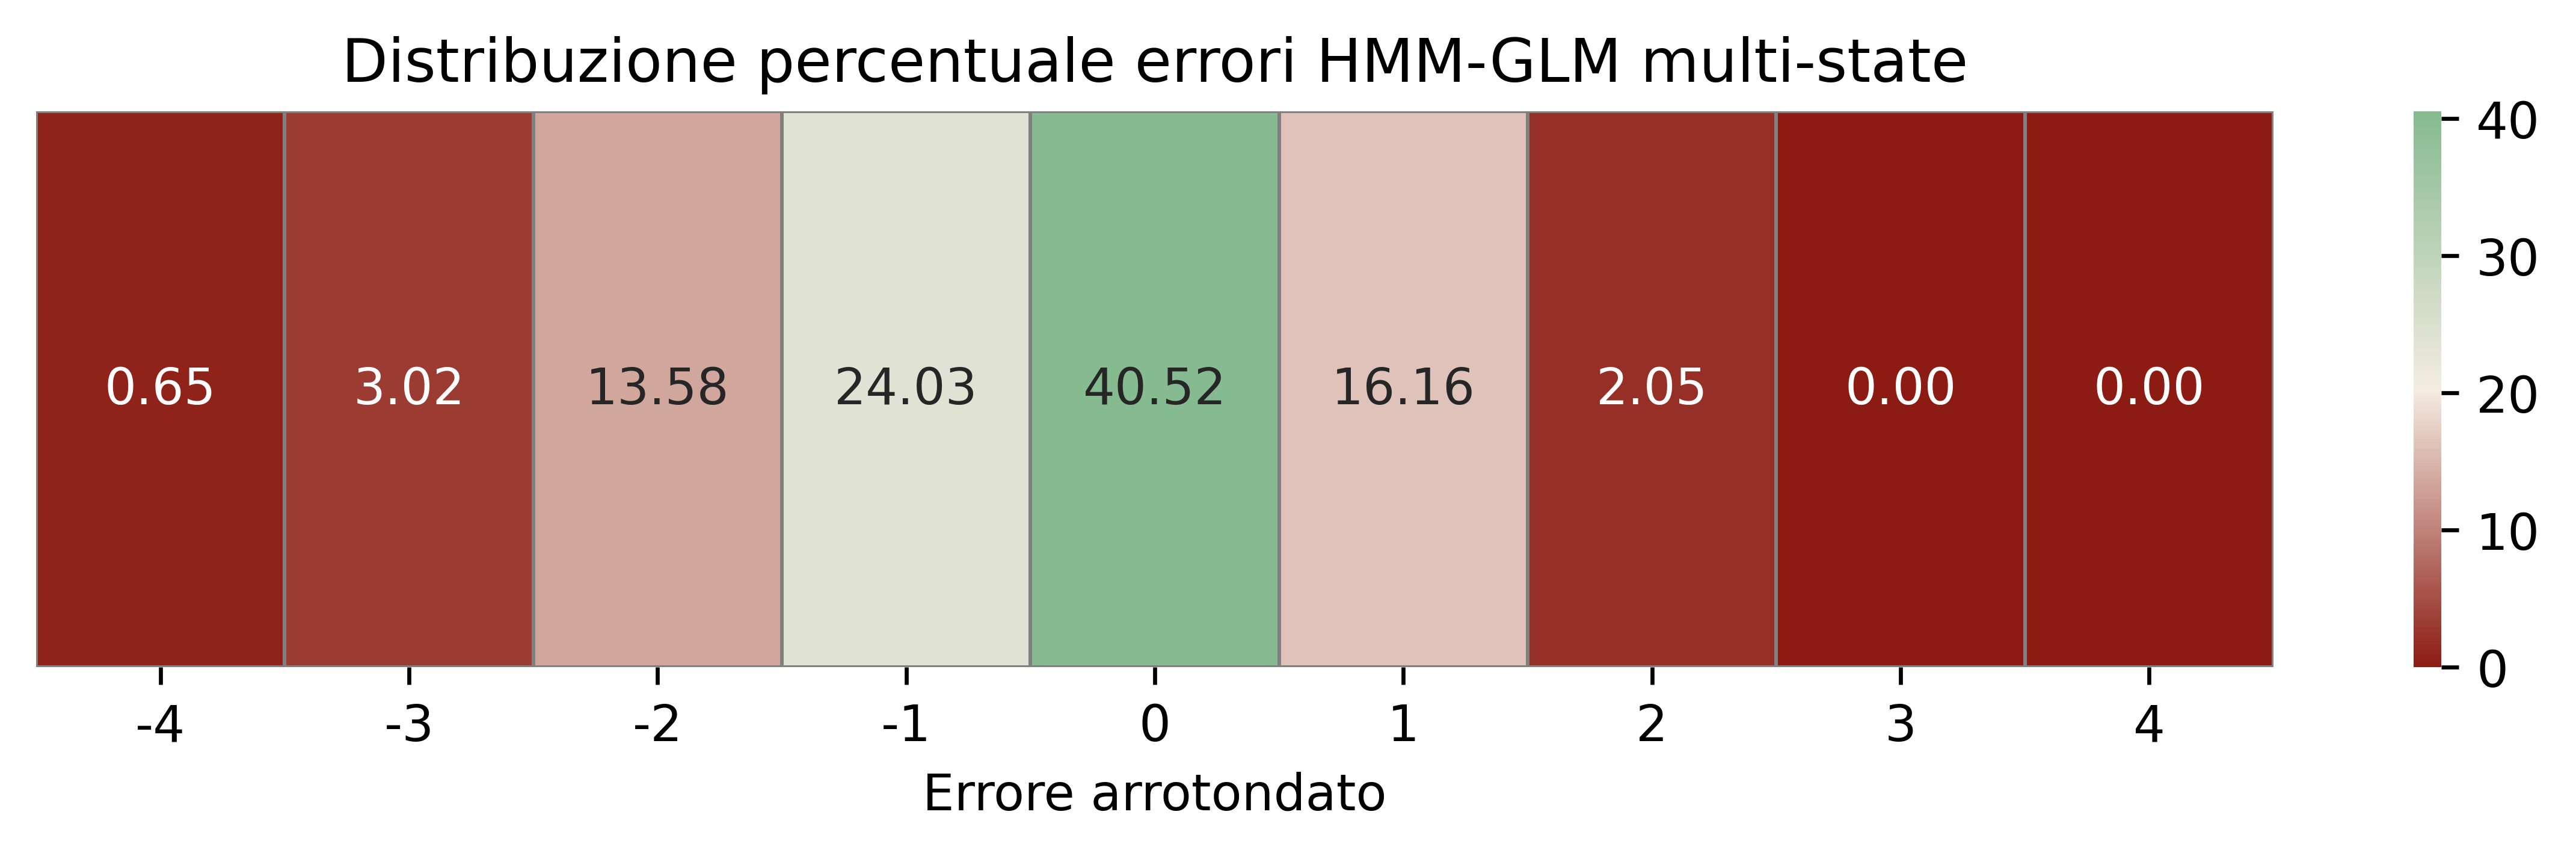
\includegraphics[keepaspectratio]{img/hmm/hmm_error_multistate_pred.png}}

}

\subcaption{\label{fig-err_hmm_ms}Errori dell'HMM-GLM considerarndo
tutti gli stati futuri}

\end{minipage}%
\newline
\begin{minipage}{\linewidth}

\centering{

\pandocbounded{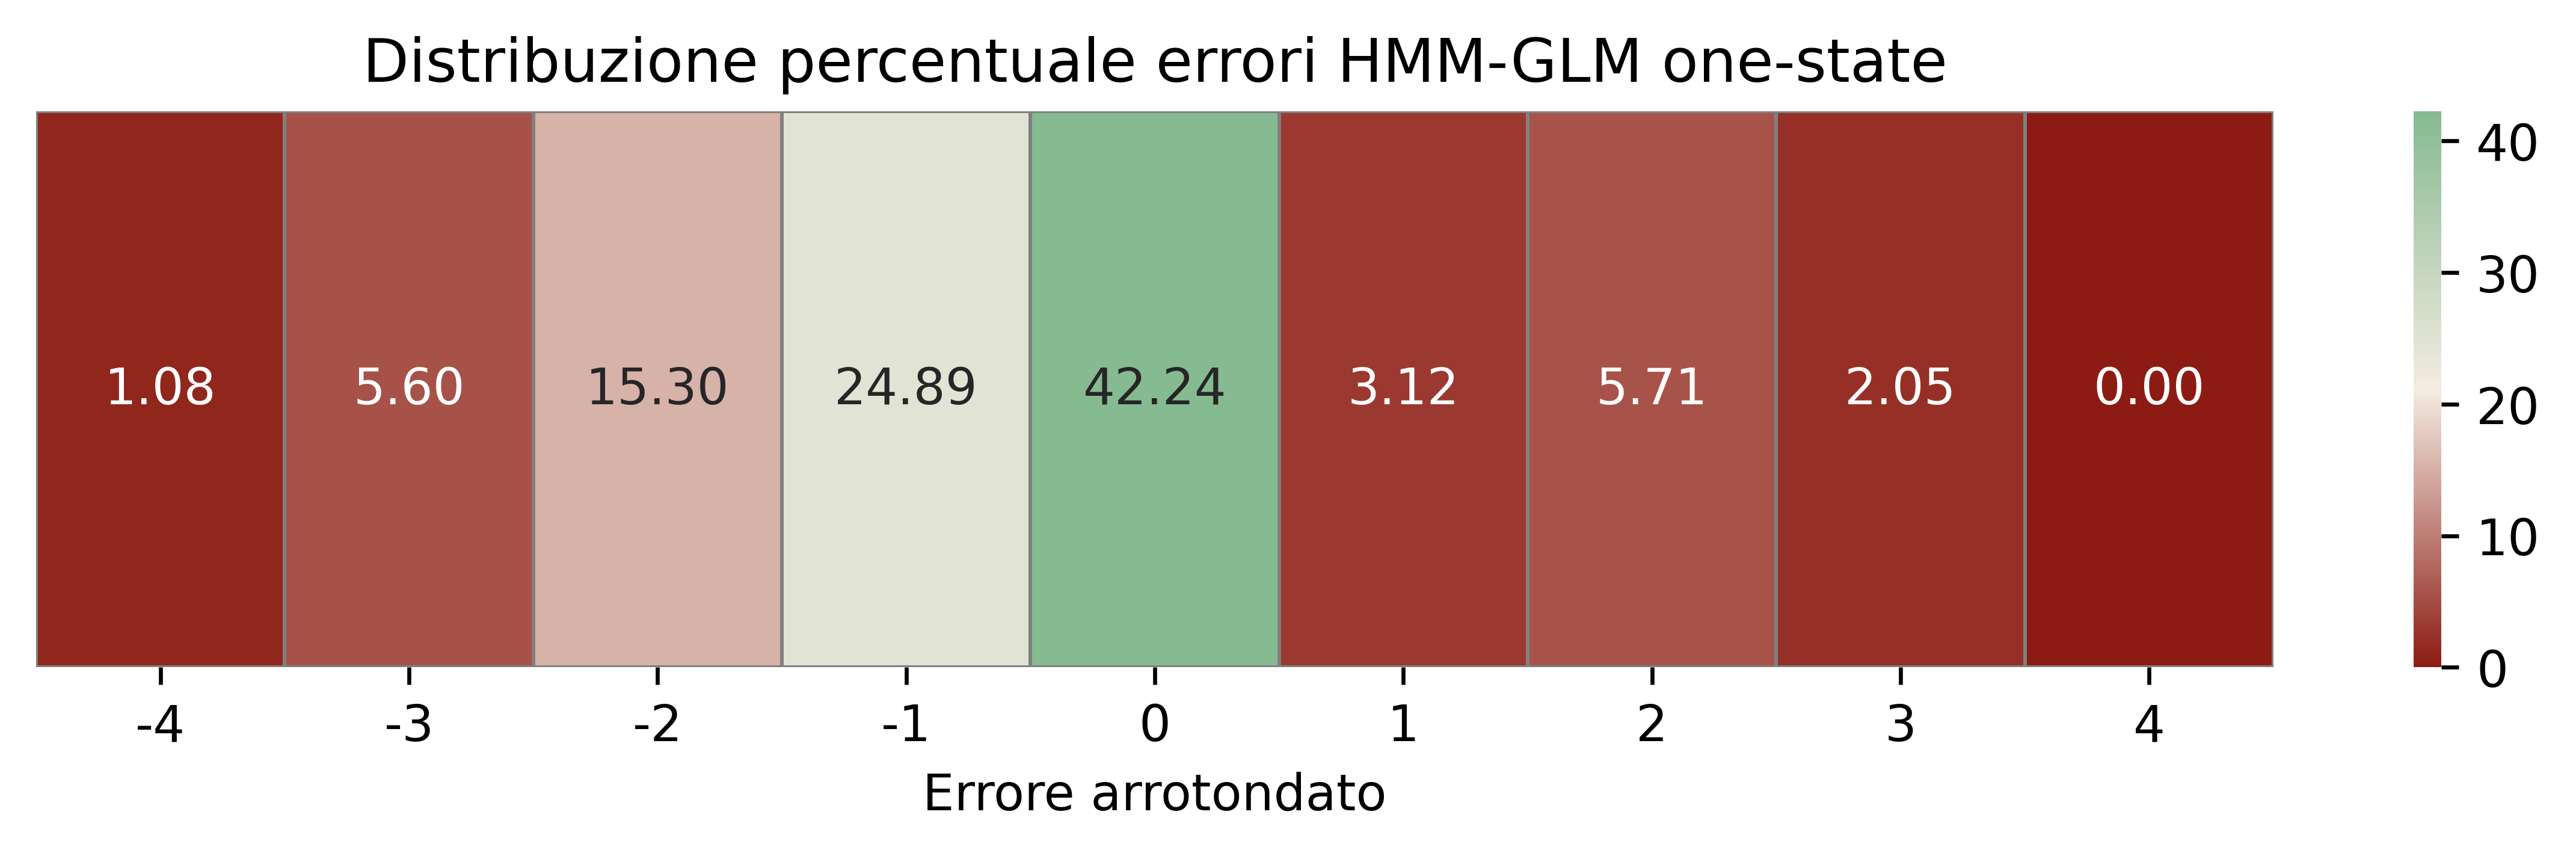
\includegraphics[keepaspectratio]{img/hmm/hmm_error_onestate_pred.png}}

}

\subcaption{\label{fig-err_hmm_os}Errori dell'HMM-GLM considerando solo
lo stato più probabile}

\end{minipage}%

\caption{\label{fig-errori}Mappe di calore sulla frequenza degli errori
per i modelli testati}

\end{figure}%

\bookmarksetup{startatroot}

\chapter{Dashboard e Sito Web}\label{dashboard-e-sito-web}

\section{Motivazione}\label{motivazione}

Lo scopo della tesi non è solo lo studio e l'analisi di un fenomeno da
parte del candidato. La tesi in questione si propone come soluzione a un
problema reale. Essa unisce la teoria alla pratica, il prodotto
dev'essere qualcosa di tangibile e facilmente usufruibile. Se per il
modello esplicativo è sufficiente esporre graficamente o tabularmente i
risultati, per il modello predittivo bisogna fare qualcosa di più,
bisogna creare uno strumento \emph{on demand}, che funzioni in tempo
reale. Come dice il nome stesso, lo scopo del modello predittivo è
quello di calcolare il valore che ci si attende da una variabile date
delle variabili di input. Il calcolo può essere svolto manualmente per
un GLM, ma già per un modello come l'HMM-GLM visto nel capitolo
precedente, il suo calcolo diventa notevolmente più complesso e
l'utilizzo di un calcolatore risulta strettamente necessario.

La dashboard si propone, quindi, come il calcolatore da utilizzare.
Dovrà rappresentare qualcosa di complesso in modo semplice e di facile
utilizzo. Lo strumento che si andrà a costruire è pensato per il
personale medico, in modo da valutare la \emph{retention} degli attuali
donatori e fare stime sui loro flussi futuri. Sarà possibile utilizzare
la dashboard da un qualsiasi dispositvo, che sia un computer o un
telefono, infatti sarà disponibile online e i calcoli verranno eseguiti
da un server.

\section{Sviluppo}\label{sviluppo}

Come il sito web ospitante la tesi, anche la dashboard è sviluppata
attraverso il \emph{framework} \href{https://quarto.org/}{Quarto}: un
sistema open-source di \emph{publishing} tecnico scientifico che
permette di sviluppare progetti in diversi formati contemporaneamente
agevolando l'interazione tra diversi linguaggi di programmazione.

Nell'ambito delle dashboard \textbf{Quarto} si occupa maggiormente della
parte \emph{front-end}, ovvero dell'interfaccia grafica. Quarto
trasforma dei documenti in stile markdown in eleganti UI (\emph{User
Interface}) in HTML, ottimizzati anche per la visualizzazione da
dispositivi mobili.

Per la parte di \emph{back-end}, ovvero la parte di server, il sistema
utilizzato è \textbf{Shiny}. Shiny è sviluppato prinicpalmente per R, ma
supporta anche Python e allo scopo di questo progetto verrà utilizzata
la versione \emph{Shiny for Python}.

I modelli e i dati sono già stati elaborati in precedenza in specifici
file Python. Riducendo così il tempo di apertura dell'applicazione.

L'attuale implementazione è ospitata su un server esterno, garantendo
così una protezione parziale dei dati che, pur essendo anonimizzati,
rappresentano comunque una risorsa da salvaguardare. Per questo motivo
l'opzione di una dashboard \emph{serverless}, ossia una soluzione adatta
a siti statici come quello che ospita la tesi, è stata scartata sia per
la quantità sia per la sensibilità delle informazioni. Infatti, in
dashboard statiche come le \emph{Shiny live}, l'interattività è gestita
tramite JavaScript e altro codice eseguito direttamente sul computer del
visitatore, implicando il trasferimento del database stesso.

\section{Struttura}\label{struttura}

L'applicazione sarà divisa in due sezioni principali: la prima dedicata
alla visualizzazione delle previsioni di stati e donazioni negli anni
futuri per le unità già presenti nei dati e un'altra che permette la
completa personalizzazione e compilazione di nuove unità, inserendo le
loro informazioni demografiche, la loro storia passata di donazioni.

La prima sezione sarà composta da una \emph{sidebar}, ovvero una barra
laterale ove inserire i dati in input, in questo caso basterà inserire
l'identificativo numerico del donatore. Il server andrà, quindi, a
interrogare il database contenente sia le donazioni, ma anche già i
\emph{path} predetti dal modello tramite l'algoritmo viterbi. Una volta
interrogato, stamperà il grafico con le donazioni, gli stati più
probabili nel passato e nel futuro e il numero di donazioni predette.
Inoltre, saranno presenti anche dei \emph{value box}, utili per mostrare
singoli dati. In questo caso verrà mostrata la probabilità di donare
l'anno successivo, il numero atteso di donazioni e le probabilità si
appartenere a ciascun stato..

La seconda sezione avrà una struttura simile, ma con una \emph{sidebar}
più ricca di contenuti. In questo caso, dovremo inserire tutti i
parametri in input necessari al modello, quindi:

\begin{itemize}
\item
  l'anno di nascita o l'età;
\item
  il genere;
\item
  una serie storica con ultime donazioni osservate.
\end{itemize}

Successivamente tramite l'algoritmo verranno predetti gli stati e il
numero di donazioni attese all'anno successivo, con una struttura simile
a quella della sezione precedente.

\bookmarksetup{startatroot}

\chapter{Conclusioni}\label{conclusioni}

Lo studio ha portato a interessanti risultati e al contempo a
evidenziato diverse lacune e difficoltà. Riassumeremo di seguito questi
punti aggiungendo anche spunti per poter continuare gli studi futuri.

\section{Punti di forza}\label{punti-di-forza}

L'analisi ha giovato di un dataset pulito. Un altro studente
dell'università di Trieste si era occupato in precedenza di elaborare i
dati e svolgere delle analisi preliminari. Ciò ha permesso di partire
direttamente da un insieme di dati coerente e il processo di pulizia è
stato minimo.

Un'altra caratteristica positiva è stata il grande numero di
osservazioni in proporzione al numero di covariate disponibili. Questo
ha aiutato l'elaborazione del modello HMM-GLM, permettendo quindi di
raggruppare (\emph{clusterizzare}) per ogni anno i donatori ed usare un
modello differente per ciascun gruppo, o il modello mistura di tutti
quanti. Si evidenzia, inoltre, come questa clusterizzazione è dinamica e
in continuo movimento, questo raggruppamento è capace di adattarsi al
complesso e mutabile comportamento umano.

La tesi è riuscita a far ``parlare'' le variabili, i modelli hanno
svelato pattern nascosti, più complessi e difficilmente ottenibile
dall'inserimento delle semplici covariate date. A dimostrazione che una
profonda analisi e conoscenza del problema e di statistica è a dir poco
necessaria per la definizione di un modello capace di modellare la
realtà. Si ricorda infatti che non esiste \emph{il modello} adatto al
fenomeno oggetto di studio. Piuttosto, esiste \emph{un modello} che
interseca al meglio la natura dei dati e l'interesse di studio della
statistica. Come disse Box:

\begin{quote}
\emph{``All models are wrong, but some are useful.''}\\
--- George E. P. Box (1976)
\end{quote}

\section{Criticità riscontrate}\label{criticituxe0-riscontrate}

Questo percorso non è stato sempre roseo e rettilineo. Sono state
riscontrate diverse criticità nello sviluppo dell'analisi. Il principale
problema è stata la mancanza di informazioni socio-demografiche sui
donatori, che ha limitato decisamente l'analisi. Se da un lato
quest'assenza d'informazione ha penalizzato lo sviluppo di modelli
\emph{potenti} con decine o centinaia di predittori, che andavano alla
ricerca puramente della miglior metrica; in questo caso l'analisi si è
concentrata nel modellare il modello, piuttosto che modellare i dati,
conducendo un lavoro di limazione. In principio si è provato ad
aggiungere dati esterni come il numero di residenti nel capoluogo, per
stimare la popolazione non donante. Tuttavia, l'analisi era condotta sui
singoli individui e ciò non avrebbe giovato granché. L'integrazione di
questi dati sarebbe stata utili in un modello basato sulla serie storica
aggregata.

Il problema, inoltre, è stato limitato unicamente alle donazioni di
sangue, scartando in prinicipio gli altri tipi di donazione, come il
plasma. La decisione è stata presa in modo da semplificare il modello ed
avere un numero di donazioni annue compreso nell'intervallo \([0,4]\).
Anche i donatori sono stati filtrati, prendendo solo donatori compresi
tra i 18 e i 70 anni d'età, ovvero in età donativa. Erano presenti poche
unità fuori da questo intervallo ma sono state scartate, sempre in
ottica di semplificazione del modello.

\section{Idee per il Futuro}\label{idee-per-il-futuro}

Nel futuro si potrebbero estendere e ricavere altre informazioni da
covariate presenti nel dataset e non utilizzate. Tra queste si evidenzia
principalmente l'informazione che il donatore abbia effettuato anche
altri tipi di donazione oltre al sangue. Questo arricchirebbe
sostanzialmente e potrebbe probabilmente portare a un \emph{quarto}
stato latente nel modello: i \emph{super}-donatori. Un'altra variabile
da considerare meglio è certamente l'anno di prima donazione che con
un'adeguata segmentazione potrebbe portare a risultati interessanti
sulle probabilità inziali.

Avendo a disposizione i dati di diversi centri trasfusionali, si
potrebbe condurre un'analisi su dati panel, prendendo diverse
informazioni sulla popolazione residente, come la densità popolativa, la
percentuale di studenti, lavoratori, pensionati, \ldots{} Queste
informazioni aggregate permetterebbero anche di inferenziare e
classificare i donatori partendo dai dati anonimi.

Nel modello HMM-GLM è stato utilizzato un approccio misto tra il
frequentista e il bayesiano. Infatti le prior sono state inserite
unicamente nella matrice di transizione e nelle probabilità iniziali.
Utilizzando una distribuzione che, seppur poco informativa (la
Dirchilet), comunque portava informazione in quanto erano asimmetriche
(Sezione~\ref{sec-bayesiano}) e parzialmente limitate durante
l'ottimizzazione del modello (Sezione~\ref{sec-guide}). Nelle successive
estensioni si potrebbe implementare l'utilizzo di hyper-prior sui
parametri delle prior e l'introduzione di prior anche sulle altre
componenti del modello, come i coefficienti delle emissioni. Questa
parte, però, richiederebbe anche una revisione dei successivi algoritimi
implementati e usati per le diagnostiche del modello
(Sezione~\ref{sec-forward}).

\bookmarksetup{startatroot}

\chapter*{Riferimenti}\label{riferimenti}
\addcontentsline{toc}{chapter}{Riferimenti}

\phantomsection\label{refs}
\begin{CSLReferences}{1}{0}
\bibitem[\citeproctext]{ref-bellman1957dynamic}
Bellman, Richard Ernest. 1957. \emph{Dynamic Programming}. Princeton
University Press. \url{https://books.google.com/books?id=wdtoPwAACAAJ}.

\bibitem[\citeproctext]{ref-berry}
Berry, Lucas. 2016. {«Hybrid Hidden Markov Model and Generalized Linear
Model for Auto Insurance Premiums»}. Mathesis, Concordia University.
\url{https://spectrum.library.concordia.ca/id/eprint/982074/}.

\bibitem[\citeproctext]{ref-pyro}
Bingham, Eli, Jonathan P. Chen, Martin Jankowiak, Fritz Obermeyer,
Neeraj Pradhan, Theofanis Karaletsos, Rohit Singh, Paul Szerlip, Paul
Horsfall, e Noah D. Goodman. 2018. {«{Pyro: Deep Universal Probabilistic
Programming}»}. \emph{Journal of Machine Learning Research}.

\bibitem[\citeproctext]{ref-bishop2006}
Bishop, Christopher M. 2006. \emph{Pattern Recognition and Machine
Learning}. Springer.

\bibitem[\citeproctext]{ref-capitale_sociale}
Bordandini, Paola. 2025. {«Geografie del capitale sociale. Trent'anni di
senso civico in Italia»}. Riccardo Prandini.
\url{https://cris.unibo.it/retrieve/ee59ddb4-bdeb-4be5-8d2e-e70467252248/Donazioni\%20di\%20sangue.pdf}.

\bibitem[\citeproctext]{ref-box1976science}
Box, George EP. 1976. {«Science and statistics»}. \emph{Journal of the
American Statistical Association} 71 (356): 791--99.

\bibitem[\citeproctext]{ref-caselli_demografia}
Caselli, Graziella, Jacques Vallin, e Guillaume Wunsch. 2006.
\emph{Demografia. Analisi e sintesi}. Bologna: Il Mulino.

\bibitem[\citeproctext]{ref-tidymodels}
Couch, Simon, e Max Kuhn. 2025. \emph{stacks: Tidy Model Stacking}.
\url{https://stacks.tidymodels.org/}.

\bibitem[\citeproctext]{ref-degirmenci2014introduction}
Degirmenci, Alperen. 2014. {«Introduction to Hidden Markov Models»}.
\url{https://scholar.harvard.edu/files/adegirmenci/files/hmm_adegirmenci_2014.pdf}.

\bibitem[\citeproctext]{ref-fan2015}
Fan, Jieyu. 2015. {«On Markov and Hidden Markov Models with Applications
to Trajectories»}.

\bibitem[\citeproctext]{ref-guglielmetti_mugion_2021_blood_donation_propensity}
Guglielmetti Mugion, Roberta, Maria Giovina Pasca, Laura Di Pietro, e
Maria Francesca Renzi. 2021. {«Promoting the propensity for blood
donation through the understanding of its determinants»}. \emph{BMC
Health Services Research} 21 (1): 127.
\url{https://doi.org/10.1186/s12913-021-06134-8}.

\bibitem[\citeproctext]{ref-hastie2009elements}
Hastie, T., R. Tibshirani, e J. Friedman. 2009. \emph{The Elements of
Statistical Learning}. 2nd ed. Springer.

\bibitem[\citeproctext]{ref-hoffman_svi}
Hoffman, Matthew D., David M. Blei, Chong Wang, e John Paisley. 2013.
{«Stochastic Variational Inference»}. \emph{Journal of Machine Learning
Research}.

\bibitem[\citeproctext]{ref-istat_bilancio_demo_2023}
ISTAT. 2023a. {«Bilancio demografico e popolazione residente:
definizioni e note metodologiche»}. Roma: Istituto Nazionale di
Statistica.

\bibitem[\citeproctext]{ref-istat_tavole_mortalita_2023}
---------. 2023b. {«Tavole di mortalità della popolazione residente:
metodi e note tecniche»}. Roma: Istituto Nazionale di Statistica.

\bibitem[\citeproctext]{ref-statistical_learning}
James, Gareth, Daniela Witten, Trevor Hastie, e Robert Tibshirani. 2013.
\emph{An Introduction to Statistical Learning}. Springer.

\bibitem[\citeproctext]{ref-levin2009}
Levin, David A., Yuval Peres, e Elizabeth L. Wilmer. 2009. \emph{Markov
Chains and Mixing Times}. American Mathematical Society.

\bibitem[\citeproctext]{ref-murphy2012}
Murphy, Kevin P. 2012. \emph{Machine Learning: A Probabilistic
Perspective}. MIT Press.

\bibitem[\citeproctext]{ref-nomisma_donazione_sangue_plasma}
Nomisma. 2024. {«Osservatorio Nazionale Donazione Sangue e Plasma»}.
\url{https://www.nomisma.it/press-area/osservatorio-nazionale-donazione-sangue-e-plasma/}.

\bibitem[\citeproctext]{ref-covid_blood_donation}
Pati, Ilaria, Claudio Velati, Carlo Mengoli, Massimo Franchini,
Francesca Masiello, Giuseppe Marano, Eva Veropalumbo, et al. 2021. {«A
forecasting model to estimate the drop in blood supplies during the
SARS‐CoV‐2 pandemic in Italy»}. \emph{Transfusion Medicine} 31 (marzo):
200--205. \url{https://doi.org/10.1111/tme.12764}.

\bibitem[\citeproctext]{ref-rsoftware}
R Core Team. 2023. \emph{R: A Language and Environment for Statistical
Computing}. Vienna, Austria: R Foundation for Statistical Computing.
\url{https://www.R-project.org/}.

\bibitem[\citeproctext]{ref-rabiner1989}
Rabiner, Lawrence R. 1989. {«A tutorial on Hidden Markov Models and
selected applications in speech recognition»}. \emph{Proceedings of the
IEEE} 77 (2): 257--86. \url{https://doi.org/10.1109/5.18626}.

\bibitem[\citeproctext]{ref-saturni2017_la_vis_di_avis}
Saturni, Vincenzo, Giorgio Fiorentini, e Elisa Ricciuti. 2017. \emph{La
Vis di Avis: La Valutazione di Impatto Economico e Sociale
dell'Associazione Volontari Italiani del Sangue}. FrancoAngeli.

\bibitem[\citeproctext]{ref-tidyverse}
Wickham, Hadley, Mara Averick, Jennifer Bryan, Winston Chang, Lucy
D'Agostino McGowan, Romain François, Garrett Grolemund, et al. 2019.
{«Welcome to the {tidyverse}»}. \emph{Journal of Open Source Software} 4
(43): 1686. \url{https://doi.org/10.21105/joss.01686}.

\bibitem[\citeproctext]{ref-bic_formula}
Wit, Ernst, Edwin van den Heuvel, e Jan-Willem Romeyn. 2012. {«"All
models are wrong...": an introduction to model uncertainty»}.
\emph{Statistica Neerlandica} 66 (3): 217--36.
\url{https://doi.org/10.1111/j.1467-9574.2012.00530.x}.

\end{CSLReferences}


\backmatter


\end{document}
